\documentclass[lang=cn,newtx,10pt,scheme=chinese]{elegantbook}
\usepackage{minipage-marginpar}
\usepackage{subfig}
\title{数字信号处理的FPGA实现}
\subtitle{系统实验(信息)课程实验报告}

\author{LiPtP}
\institute{吴健雄学院}
\date{2025年 3 月 24 日}
\bioinfo{指导老师}{张圣清}

\extrainfo{本报告使用 ElegantBook \LaTeX 模板进行编写,封面为本人拍摄。}

\setcounter{tocdepth}{3}

\logo{logo-blue.png}
\cover{cover.jpg}

% 本文档命令
\usepackage{array}
\newcommand{\ccr}[1]{\makecell{{\color{#1}\rule{1cm}{1cm}}}}

% 修改标题页的橙色带
\definecolor{customcolor}{RGB}{32,178,170}
\colorlet{coverlinecolor}{customcolor}
\usepackage{cprotect}

\addbibresource[location=local]{reference.bib} % 参考文献,不要删除

\begin{document}

\maketitle
\frontmatter

\tableofcontents

\mainmatter

% \chapter{信号的采样与重建}

\begin{introduction}
  \item 信号采样与重建流程
  \item 基于\textit{Simulink}的信号采样与重建仿真
  \item 基于\textit{MATLAB}的信号采样频谱绘制
\end{introduction}

\section{实验背景与目的}
  

本实验旨在探讨信号采样过程中的频谱变化,分析采样是否会导致信息丢失,并评估采样序列能否充分代表原始信号,同时研究如何实现不失真的信号还原。通过对奈奎斯特采样定理的理解与验证,深入分析采样频率与信号最高频率之间的关系,并研究当采样定理不满足时可能出现的频谱混叠现象及其影响。此外,实验将研究离散时间信号的采样(抽取)、插值及采样率转换的基本原理与实现方法,并观察这些操作在时域和频域中的特性变化。针对信号采样与重建过程中的关键环节,本实验还将介绍模拟低通滤波器的指标特性,包括抗混叠滤波器和平滑滤波器的作用,并探讨其设计要求及实际应用中的挑战。最终,通过 MATLAB 和 Simulink 搭建实验平台,进行信号采样与重建实验,验证理论知识,分析实验结果,并通过解决实验过程中遇到的问题,提高实践操作和数据分析能力。

\section{实验原理}

\subsection{信号采样基础}
信号采样是指对连续时间信号 $x(t)$ 按固定采样周期 $T$ 进行取值,得到离散时间信号 $x[n]$,其中:
\begin{equation}
    x[n] = x(nT), \quad n \in \mathbb{Z}.
\end{equation}
实际采样系统一般包括采样保持器(Sample-and-Hold)和模数转换器(A/D Converter)。采样保持器用于保持瞬时幅度,而 A/D 转换器完成模拟信号与数字信号的转换。

在理想采样条件下,采样过程可看作原始信号与冲激函数序列 $\delta_T (t)$ 相乘:
\begin{equation}
    x_s (t) = x(t) \sum_{n=-\infty}^{\infty} \delta (t - nT).
\end{equation}
其中,$\delta (t)$ 为单位冲激函数。当脉冲宽度 $\tau$ 远小于采样周期 $T$ 时,实际采样接近理想采样。

\subsection{采样信号的频谱特性}
在频域中,采样的本质是对原始信号的频谱 $X(\Omega)$ 进行周期延拓,采样信号的频谱表示为:
\begin{equation}
    X_s(\Omega) = \frac{1}{T} \sum_{k=-\infty}^{\infty} X\left(\Omega - k\Omega_s\right),
\end{equation}
其中 $\Omega_s = \frac{1}{T}$ 是采样频率,$\Omega$ 为连续频率变量。由此可见,采样信号的频谱是原始信号频谱的周期重复。

根据奈奎斯特采样定理,若信号的最高频率 $\Omega_{\max}$ 满足:
\begin{equation}
    \Omega_s \geq 2\Omega_{\max},
\end{equation}
则可以通过带宽为 $\Omega_s/2$ 的理想低通滤波器完美重建原信号。当 $\Omega_{\max} > \Omega_s/2$ 时,会发生\textbf{频谱混叠}(aliasing),即高频分量叠加到低频范围,导致信息损失。为了避免混叠,实际应用中通常选择更高的采样频率,并在采样前使用抗混叠低通滤波器。


\subsection{模拟低通滤波器特性}
抗混叠滤波器用于在采样前抑制高于 $\Omega_s/2$ 的频率成分,以防止频谱混叠。然而,理想低通滤波器的矩形频率响应在实际中无法实现,因此采样频率越低,对抗混叠滤波器的要求越高。

在信号重建过程中,\textbf{平滑滤波器} 主要用于去除 D/A 转换后信号中的高频成分。对于理想的平滑滤波器,其频率响应呈指数衰减,在 $\Omega = k\Omega_s$ 处取零。

\subsection{带通信号的采样}
对于带通信号,其频谱分布于 $\left[\Omega_1, \Omega_2\right]$,其中 $\Omega_2 - \Omega_1 = \Delta\Omega$ 为信号带宽。若 $\Omega_2$ 是带宽的整数倍,则可以选择欠采样方式,此时采样频率 $\Omega_s$为
\begin{equation}
    \Omega_s = 2\Delta\Omega.
\end{equation}
欠采样后,由于低频有大量带宽没有传输信号,若满足适当的带通滤波条件,仍可恢复原信号。并且如果 $\Omega_2$ 不是 $\Delta\Omega$ 的整数倍,则可通过频带扩展调整信号频谱以满足采样条件。

\subsection{离散时间信号的处理}
\begin{definition}[离散时间信号的抽取]
  抽取(Decimation) 指对信号进行降采样,即每隔 $M$ 个采样点保留一个:
\begin{equation}
    x_d[n] = x[Mn].
\end{equation}
\end{definition}

由于采样频率降低了M倍,这种信号处理方式还被称为\textbf{M倍降采样}。为了防止混叠,降采样前需使用抗混叠低通滤波器。

\begin{definition}[离散时间信号的插值]
  插值(Interpolation)指对信号进行升采样,即在相邻采样点之间插入 $L-1$ 个零值:
\begin{equation}
    x_i[n] = \begin{cases}
        x[n/L], & n = 0,  L,  2L, \ldots, \\
        0, & \text{其他}.
    \end{cases}
\end{equation}
\end{definition}

插值用于提高采样率,最简单的方法是插零,然后通过数字低通滤波器去除镜像分量。在语音信号处理等专门领域中,插入的值由专用算法指定,以获得更好的重建质量。

将抽取和插值结合起来便是\textbf{采样率转换}(Sample Rate Conversion)技术。它是指采样率按有理数 $L/M$ 进行变换的方法,通常采用先插值$L$ 倍,再抽取$M$倍的方式实现。转换过程中,在升降采样的间隙必须使用合适的低通滤波器来抑制高频成分,以避免失真。值得注意的是,这个滤波器既承担了抗混叠的作用,也起到了平滑滤波的作用。


\section{实验使用软件}
\begin{itemize}
  \item MATLAB 2024b
  \item Simulink 2024b
\end{itemize}

\section{实验内容}

\subsection{基于 Simulink 的信号采样与重建时域仿真}

利用Simulink搭建信号采样与重建仿真系统,验证信号采样与重建的基本原理。在这个实验中,我们使用正弦波通过经过采样后通过一切比雪夫低通滤波器的模型为例,分析各个阶段中信号是如何采样重建的。具体步骤如下:
\begin{itemize}
  \item 搭建实验模型,如图~\ref{fig:model1}~所示。
  \item 设置正弦波的频率为 $f = 1$ kHz,脉冲波的频率为 $f = 5$ kHz,占空比25\%。给定低通滤波器的截止频率为 $f_c = 1.5$ kHz。
  \item 启动仿真,观察\lstinline{Scope}中的波形。
\end{itemize}
\begin{figure}[htbp]
  \centering
  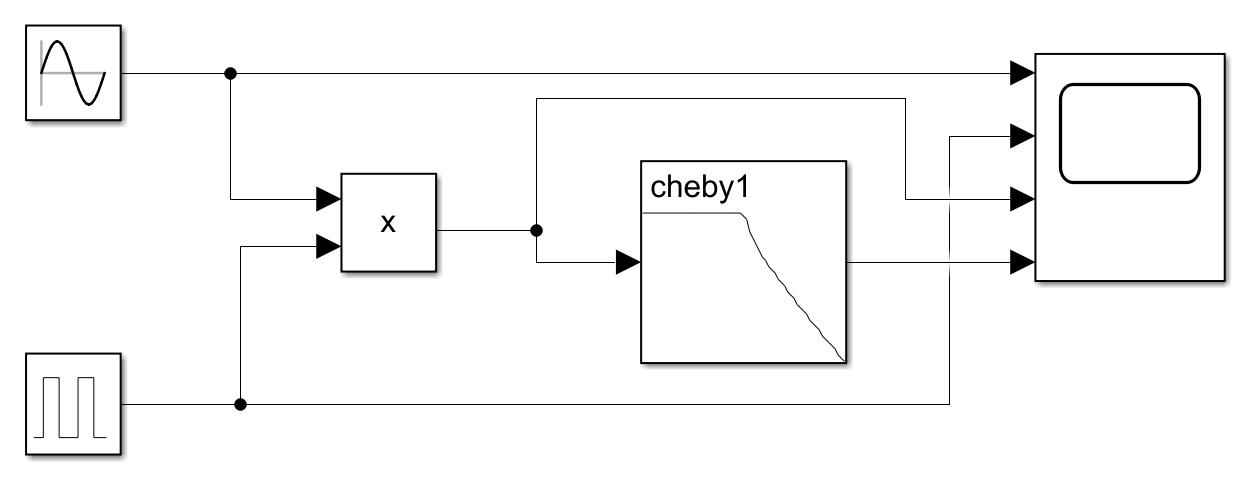
\includegraphics[width=0.5\textwidth]{figure/exp1/model1.png}
  \caption{信号采样与重建仿真模型}
  \label{fig:model1}
\end{figure}

\begin{figure}[htbp]
  \centering
  \subfloat[默认参数下的信号采样重建波形\label{fig:sim1}]{
    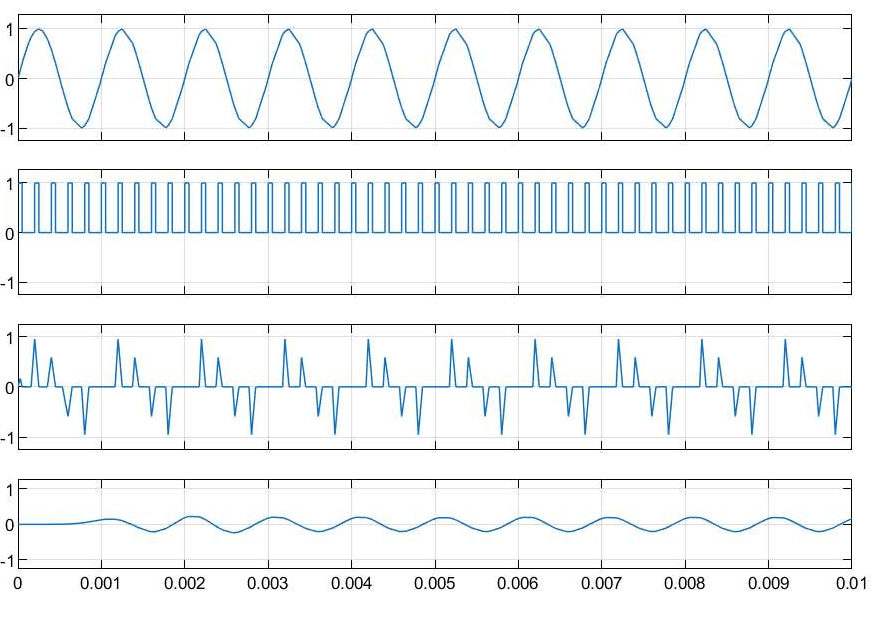
\includegraphics[width=0.45\textwidth]{figure/exp1/sim1.pdf}
  }
  \hfill
  \subfloat[$f_s$=1.5kHz时的采样重建波形\label{fig:sim2}]{
    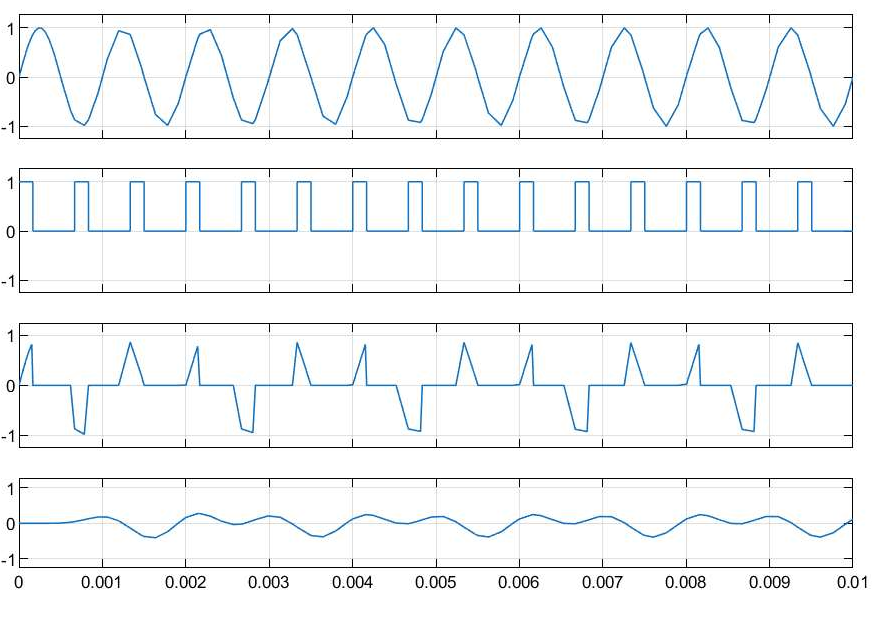
\includegraphics[width=0.45\textwidth]{figure/exp1/sim2.pdf}
  }
  \newline
  \subfloat[低通滤波器截止频率为5kHz时的信号重建\label{fig:sim3}]{
    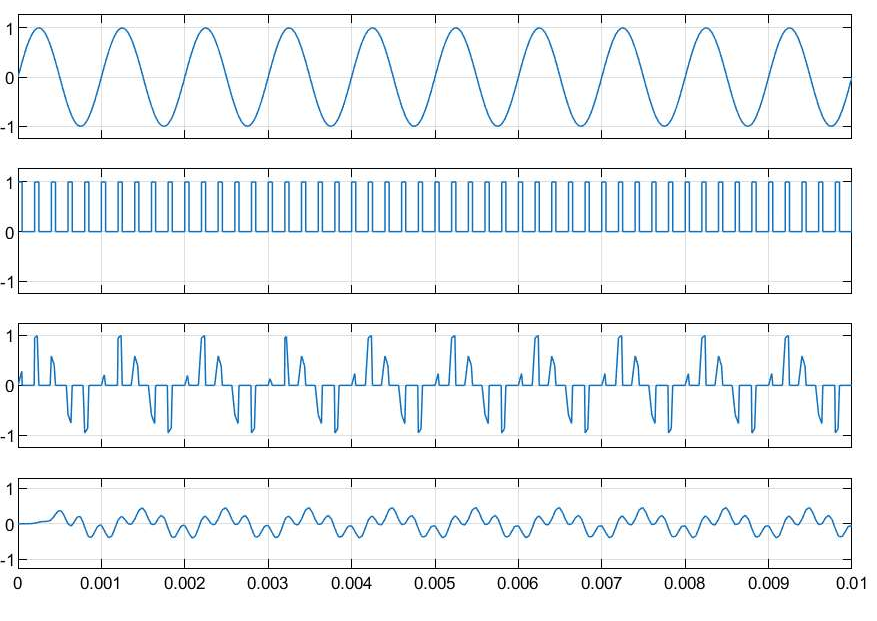
\includegraphics[width=0.45\textwidth]{figure/exp1/sim3.pdf}
  }
  \hfill
  \subfloat[冲激信号占空比50\%时的信号重建\label{fig:sim4}]{
    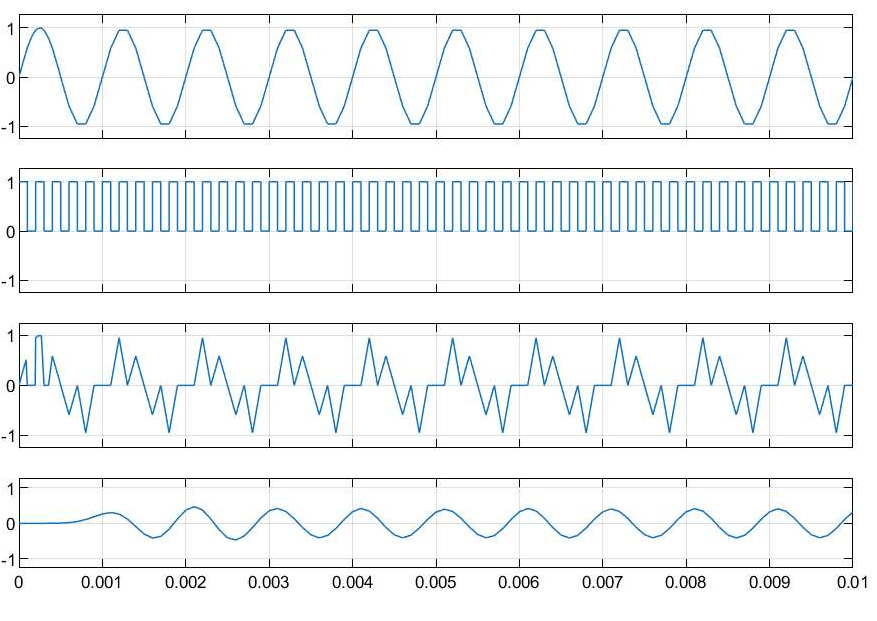
\includegraphics[width=0.45\textwidth]{figure/exp1/sim4.pdf}
  }
  \caption{信号采样与重建时域仿真结果}
  \label{fig:sim}
\end{figure}

默认参数下的仿真结果如图~\ref{fig:sim1}~所示。从上到下的四条波形分别为发射正弦波、采样冲激信号、采样信号和重建信号。可以看到,重建信号的频率与原始信号一致,但幅度有所损失。接下来,为了验证奈奎斯特采样定理,将采样频率降低为1.5kHz,重新进行仿真。仿真结果如图~\ref{fig:sim2}~所示。可以看到,重建信号“叠”在了一起,和原始信号有明显的差异。故认为该采样频率下信号出现了混叠。保持采样频率为5kHz,将低通滤波器的截止频率调整为5kHz,重新进行仿真。仿真结果如图~\ref{fig:sim3}~所示。可以看到,重建信号的频率大体上与原始信号一致,但是波形出现了抖动。这说明,低通滤波器可以滤除高频分量,从而使得重建信号更加平滑。最后,为了验证脉冲信号宽度对重建信号性能的影响,将脉冲信号占空比调至50\%,观察仿真波形如图~\ref{fig:sim4}~所示。可以看到采样信号和重建信号的幅值都变大了,这是由于脉冲信号的占空比增大,使得采样信号的幅值增大。


\subsection{基于Simulink的信号采样仿真}

在进行模型时域波形仿真后,进一步利用Simulink分析信号采样的频谱特性。具体步骤如下:
\begin{itemize}
  \item 搭建实验模型,如图~\ref{fig:model2}~所示。
  \item 设置三个正弦波发生器的频率分别为 $f_1 = 500$ kHz,$f_2 = 4400$ kHz,$f_3 = 5800$ kHz。设置合成波的三种采样频率分别为30MHz,10MHz和3MHz,幅值分别为10,5,1。\footnote{按照课上讲义,这里取了更高的采样频率以免显示不全。}
  \item 启动仿真,观察\lstinline{Scope},\lstinline{Scope1}和\lstinline{Spectrum Analyzer}中的频谱。

\end{itemize}

\begin{figure}[htbp]
  \centering
  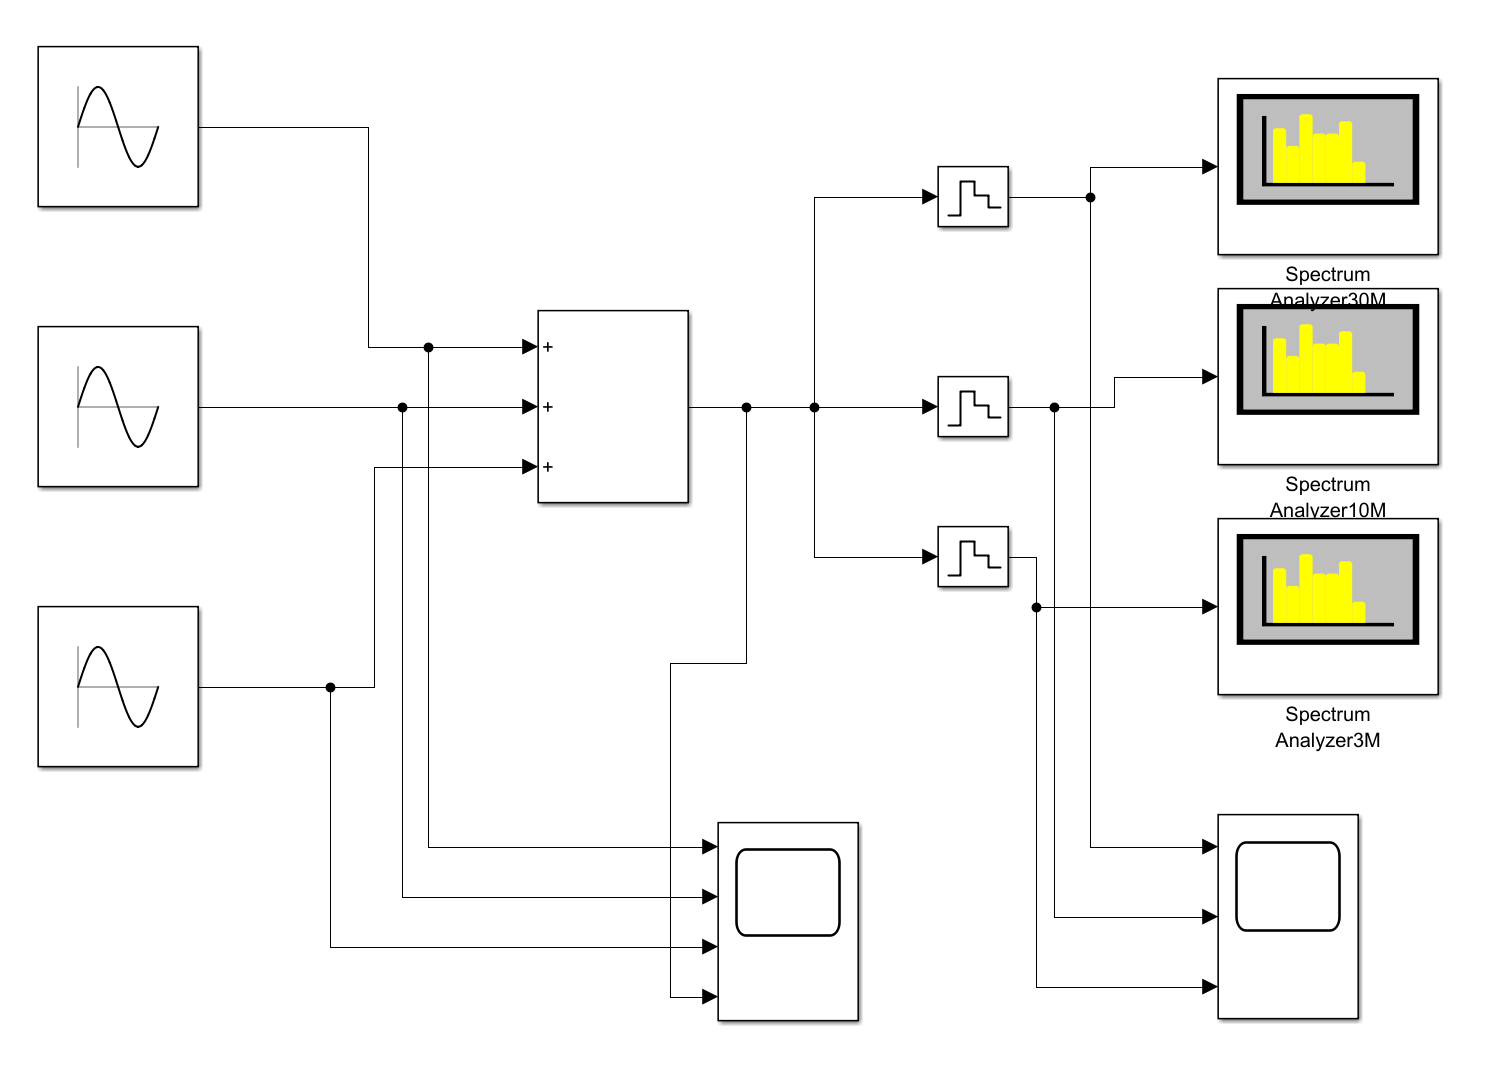
\includegraphics[width=0.65\textwidth]{figure/exp1/model2.png}
  \caption{信号采样与重建频域仿真模型}
  \label{fig:model2}
\end{figure}

启动仿真后,首先观察\lstinline{Scope}的结果,如图~\ref{fig:sim2_1}~所示。使用青蓝色标注第一个频率为$f_1$的正弦波,使用天蓝色标注第二个频率为$f_2$的正弦波,使用黄绿色标注第三个频率为$f_3$的正弦波,并用墨绿色标注通过加法器后的正弦波。可以看到,三个正弦波的频率分别为500kHz,4400kHz和5800kHz。通过加法器的正弦波周期为三个正弦波周期的最小公倍数,因此频率最小。

接下来,观察\lstinline{Scope1}的结果,如图~\ref{fig:sim2_2}所示。使用青蓝色标注采样频率为$f_{s1} = 30$MHz的波形,使用天蓝色标注采样频率为$f_{s2} = 10$MHz的波形,使用黄绿色采样频率为$f_{s3} = 3$MHz的波形。可以看到,加和正弦波的频率通过保持器后保持不变,但变成了阶跃形的波形。采样频率越高,阶跃次数越多,越贴近真波形。

最后,观察\lstinline{Spectrum Analyzer}的结果如图~\ref{fig:spectrum30}~、~\ref{fig:spectrum10}~、~\ref{fig:spectrum3}~所示。观察对称频谱的峰值,可以看到清晰的三根谱线。在前两个图中,信号的峰值出现在预设频率 0.5 MHz、4.4 MHz 和 5.8 MHz 附近,且幅度经过V/dBm的$20\log$计算公式换算后保持一致。三个峰值中,最大值与最小值的差异约为 20 dB,与理论计算结果一致。然而,在采样频率为10MHz的结果中,频率峰值偏离了设定值,这可能是由于该频率分量与FFT采样点不对齐导致的栅栏效应,或者该频率分量出现了泄露。  



\begin{figure}[htbp]
    \centering
    \subfloat[采样前的时域波形\label{fig:sim2_1}]{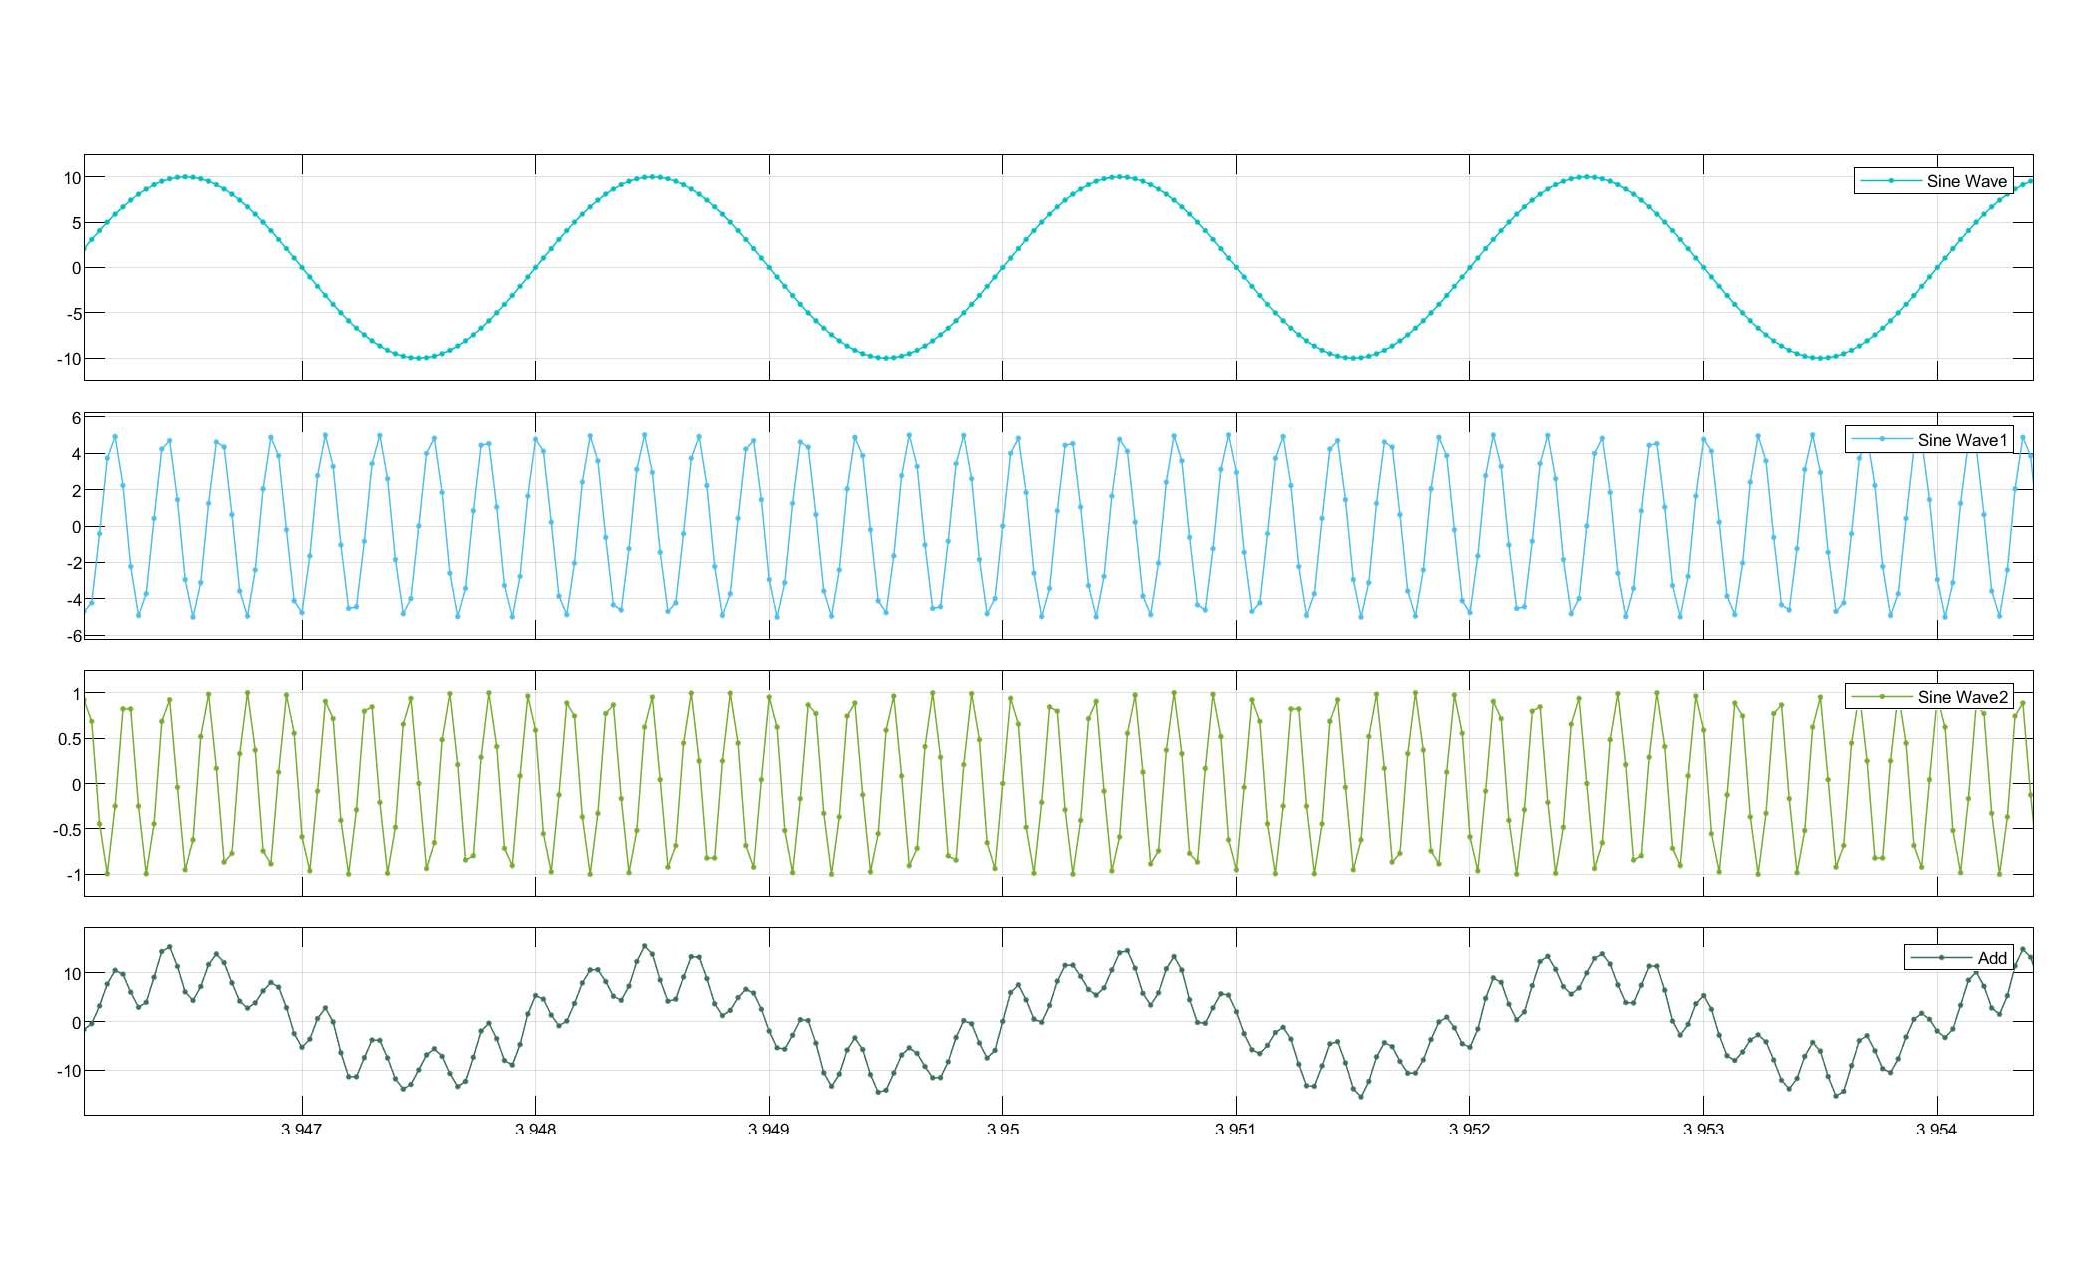
\includegraphics[width=0.95\textwidth]{figure/exp1/sim2_1.pdf}}
    \newline
    \subfloat[采样后的时域波形\label{fig:sim2_2}]{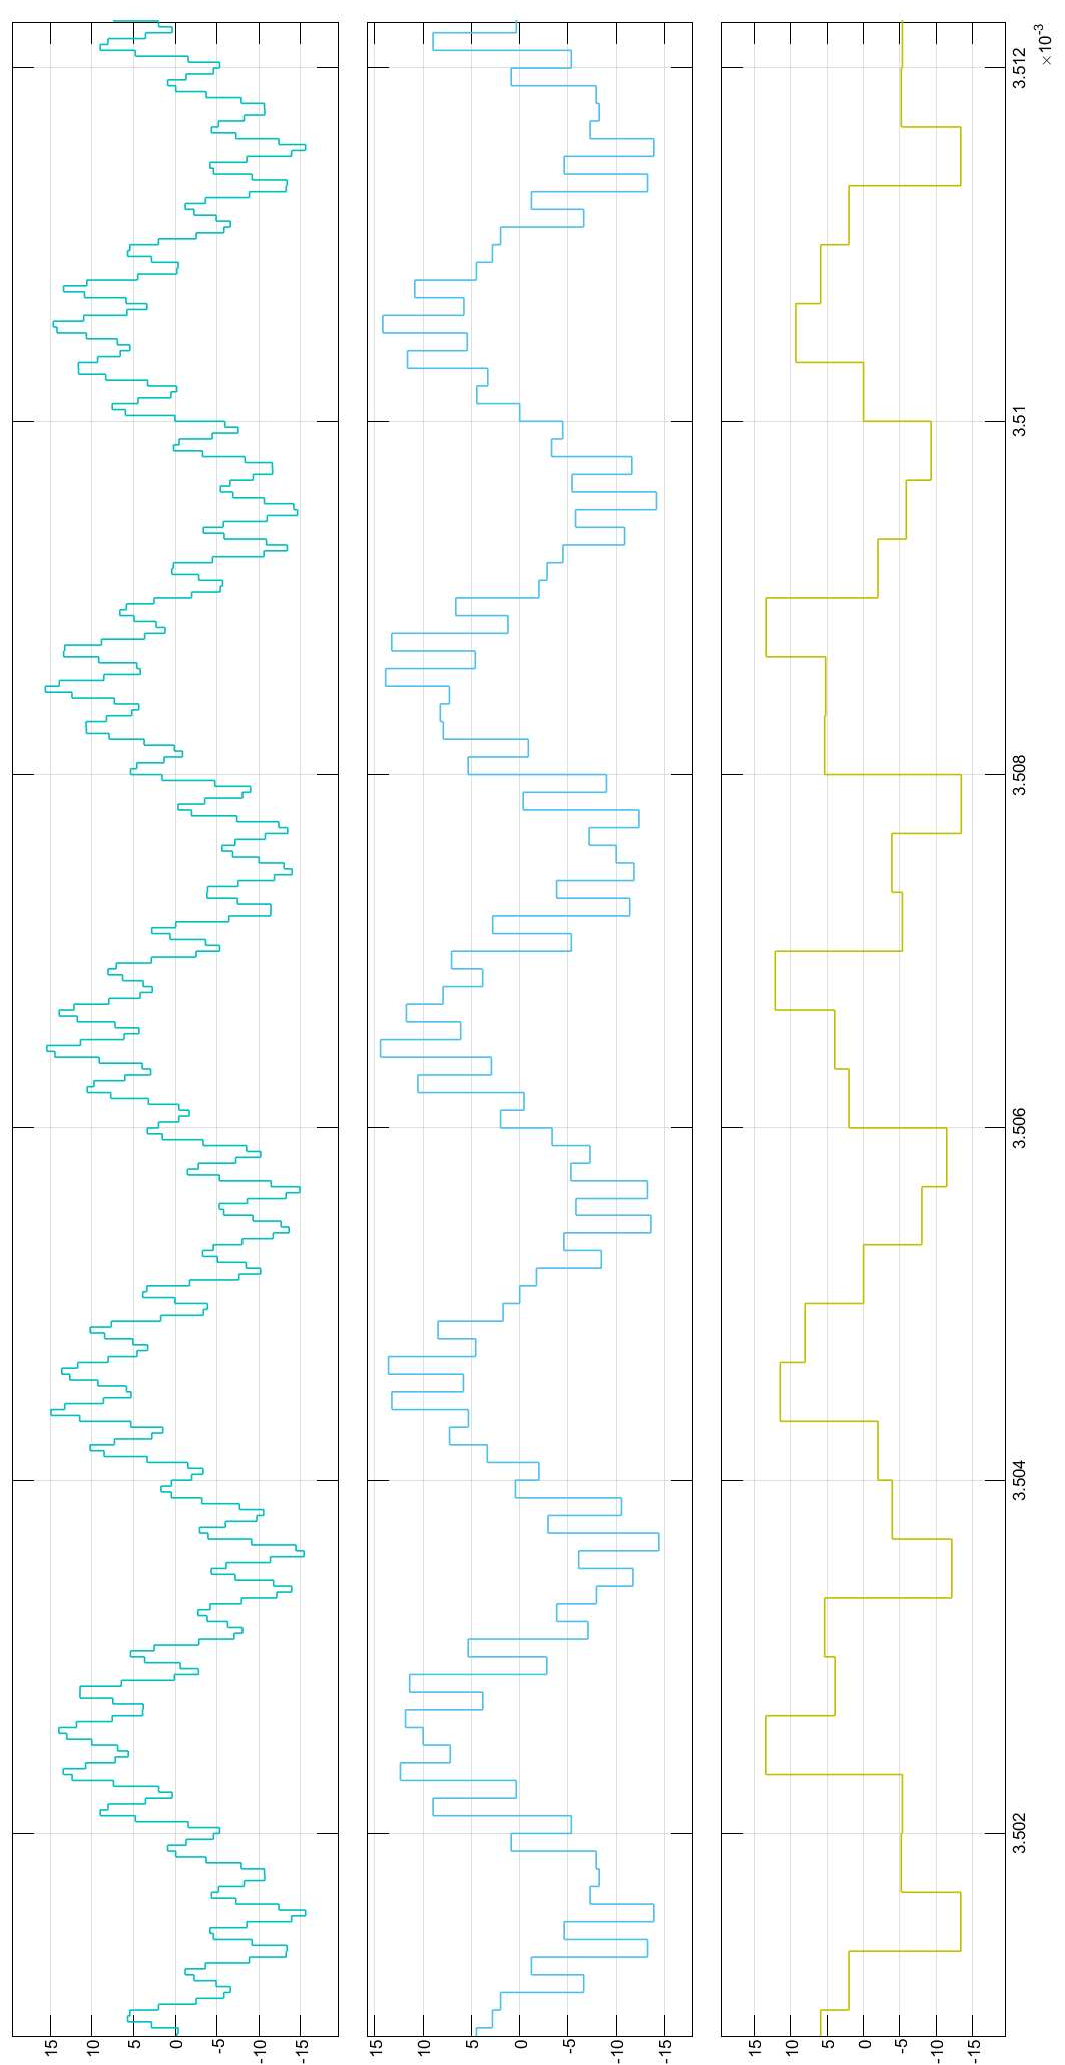
\includegraphics[width=0.47\textwidth,angle=-90]{figure/exp1/sim2_2.pdf}}
    \caption{时域波形仿真结果}
\end{figure}
\begin{figure}[htbp]
  \centering
  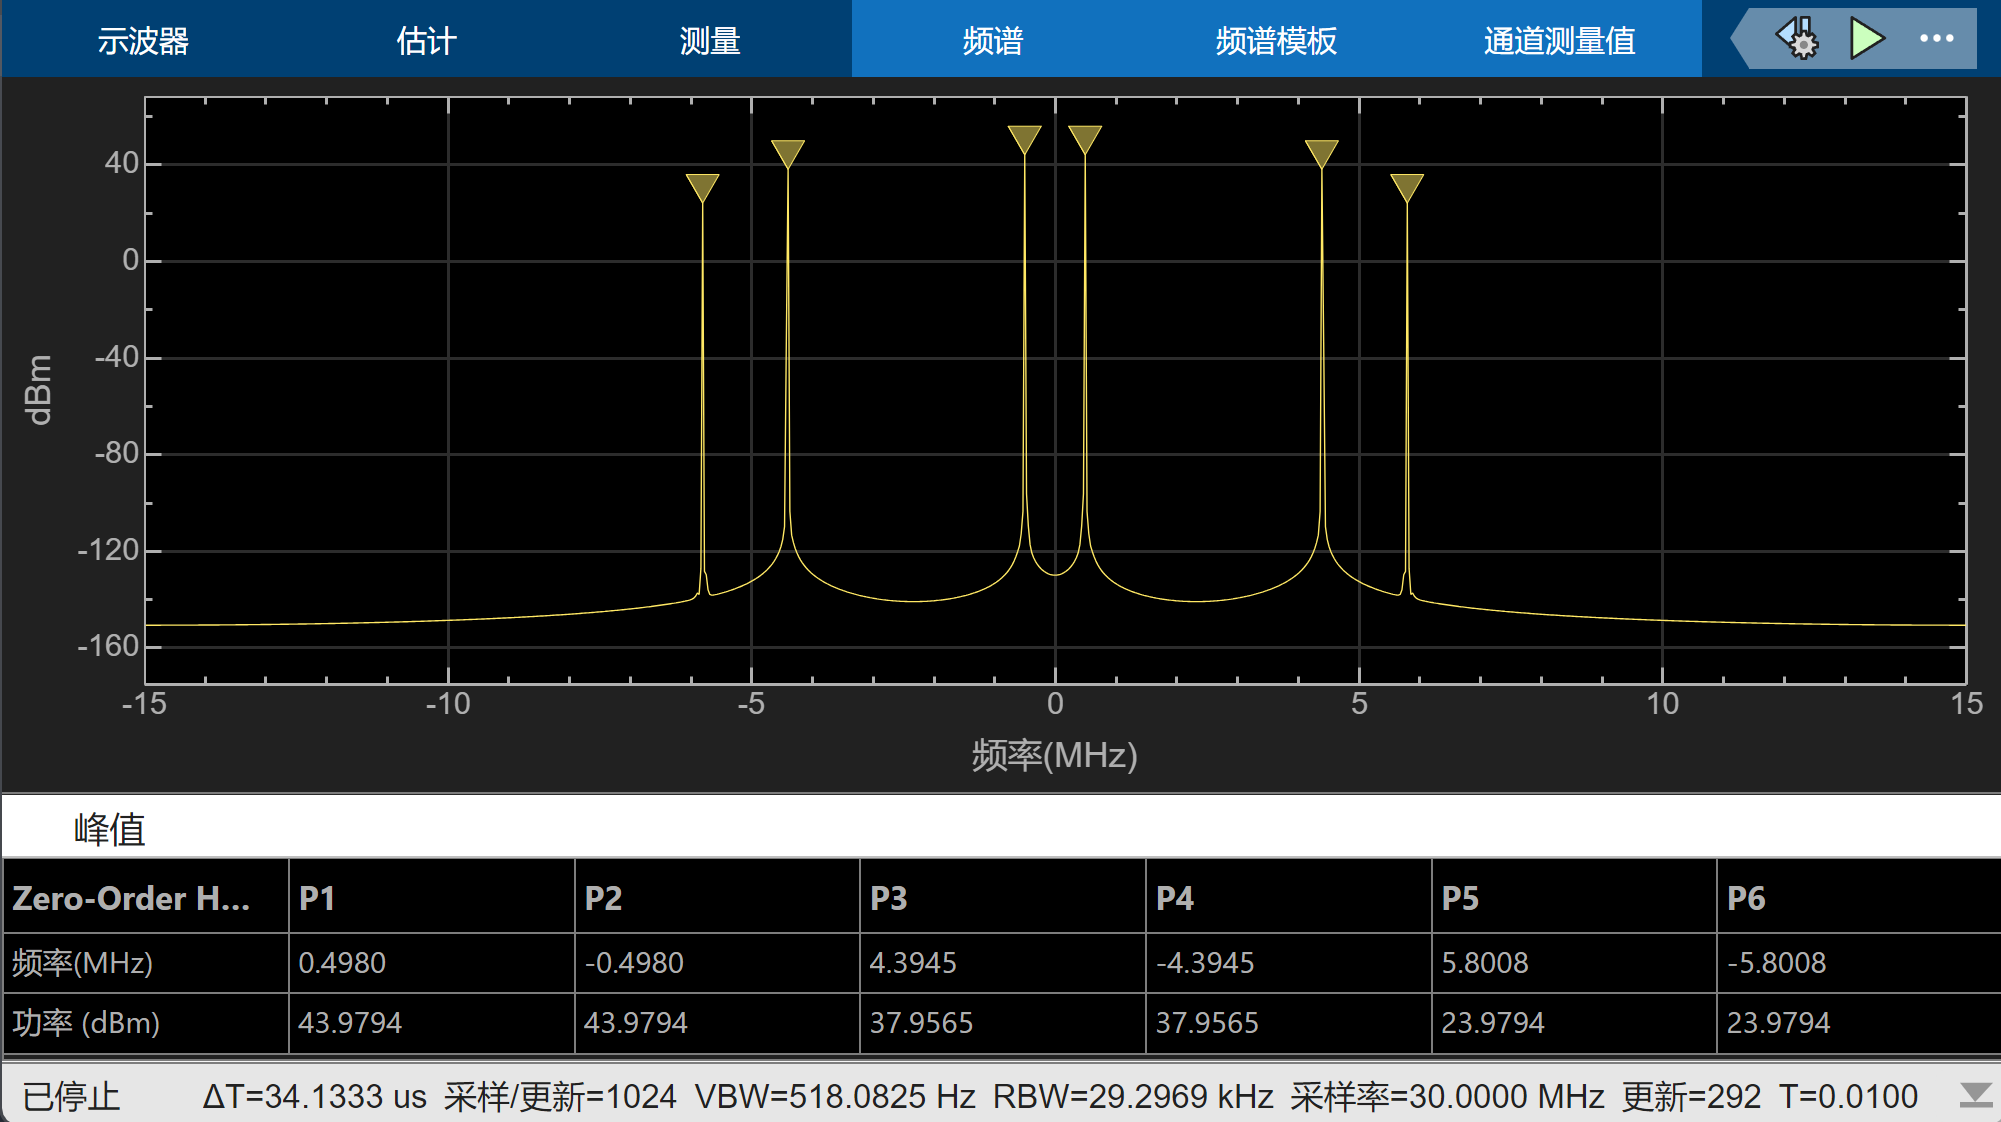
\includegraphics[width=0.75\textwidth]{figure/exp1/30M.png}
  \caption{采样频率为30MHz下的输出频谱}
  \label{fig:spectrum30}
\end{figure}
\begin{figure}[htbp]
  \centering
  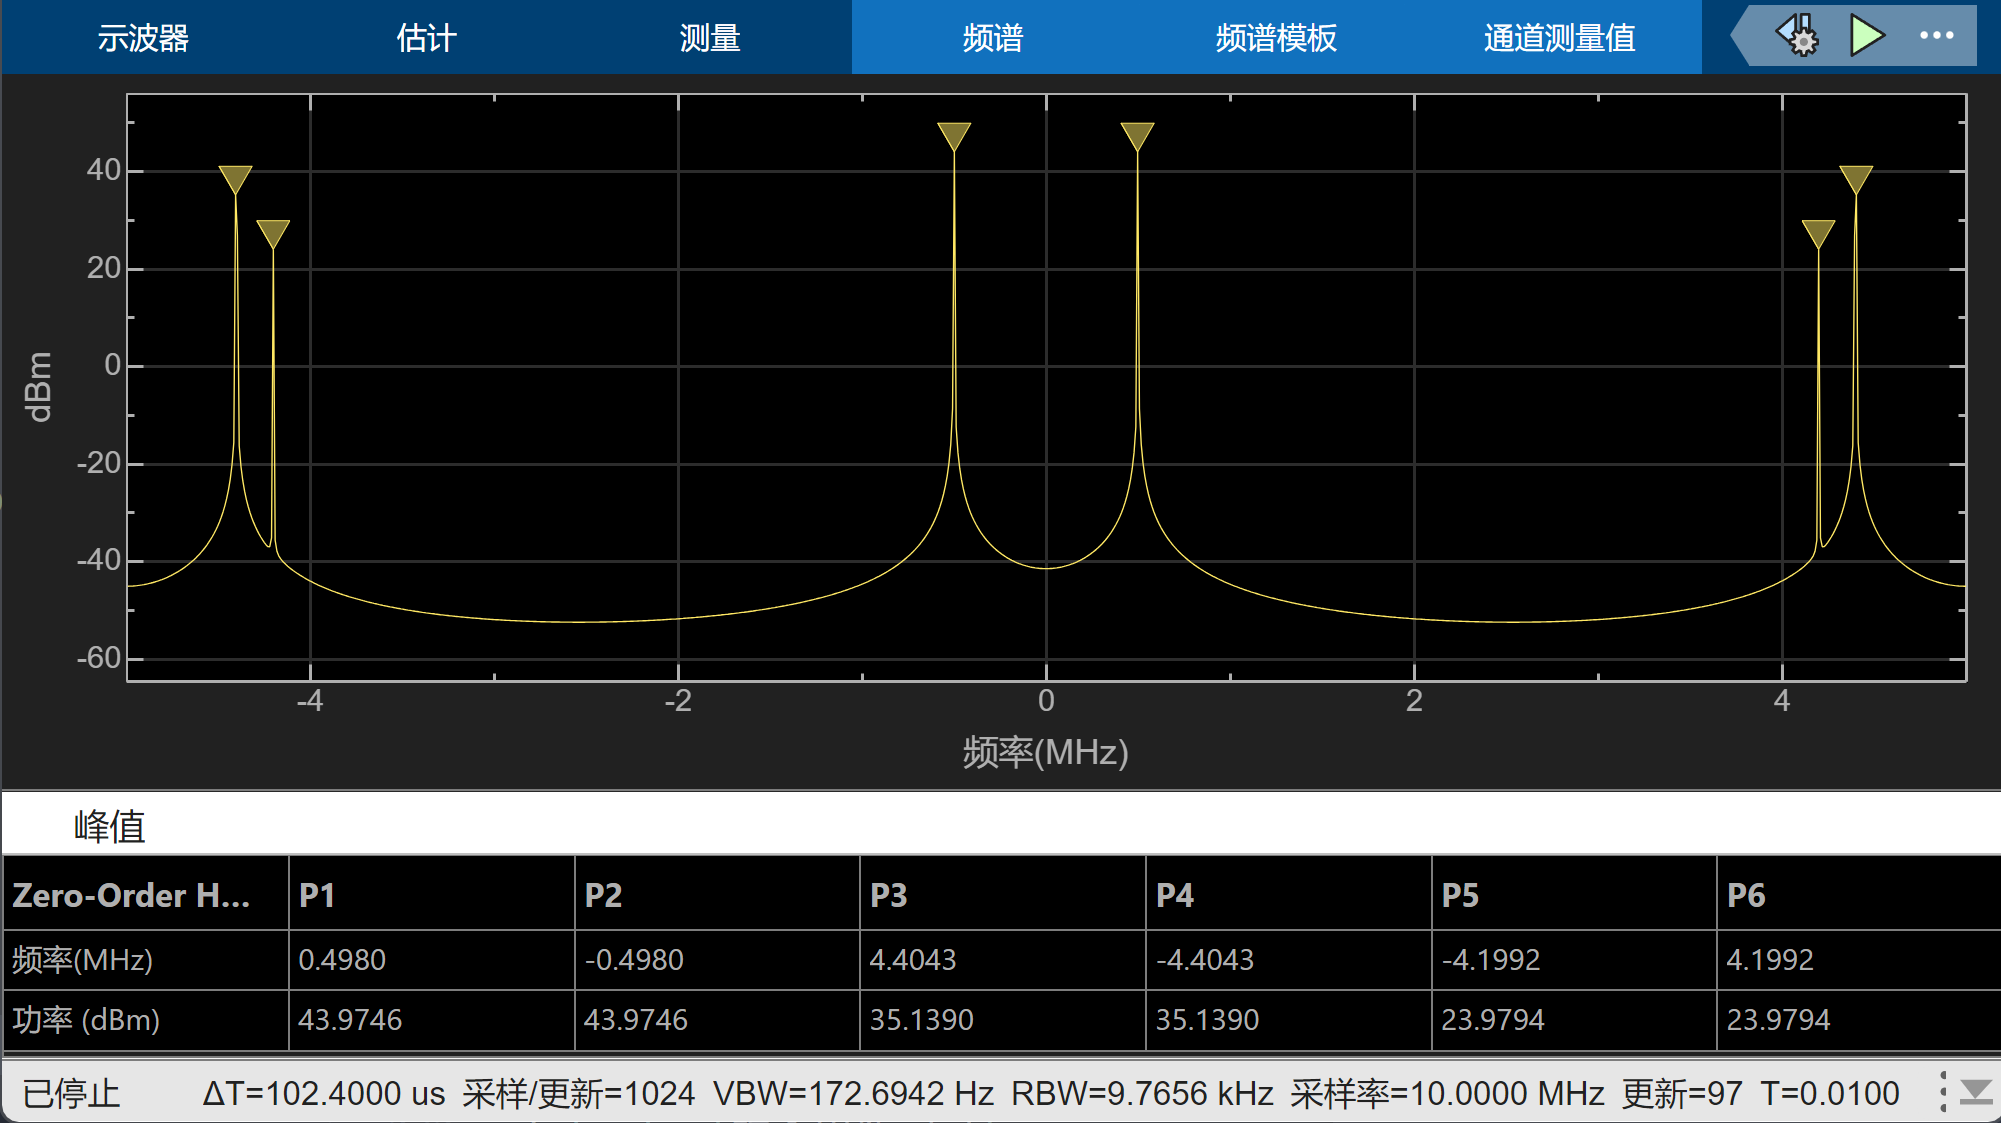
\includegraphics[width=.75\textwidth]{figure/exp1/10M.png}
  \caption{采样频率为10MHz下的输出频谱}
  \label{fig:spectrum10}
\end{figure}
\begin{figure}[htbp]
  \centering
  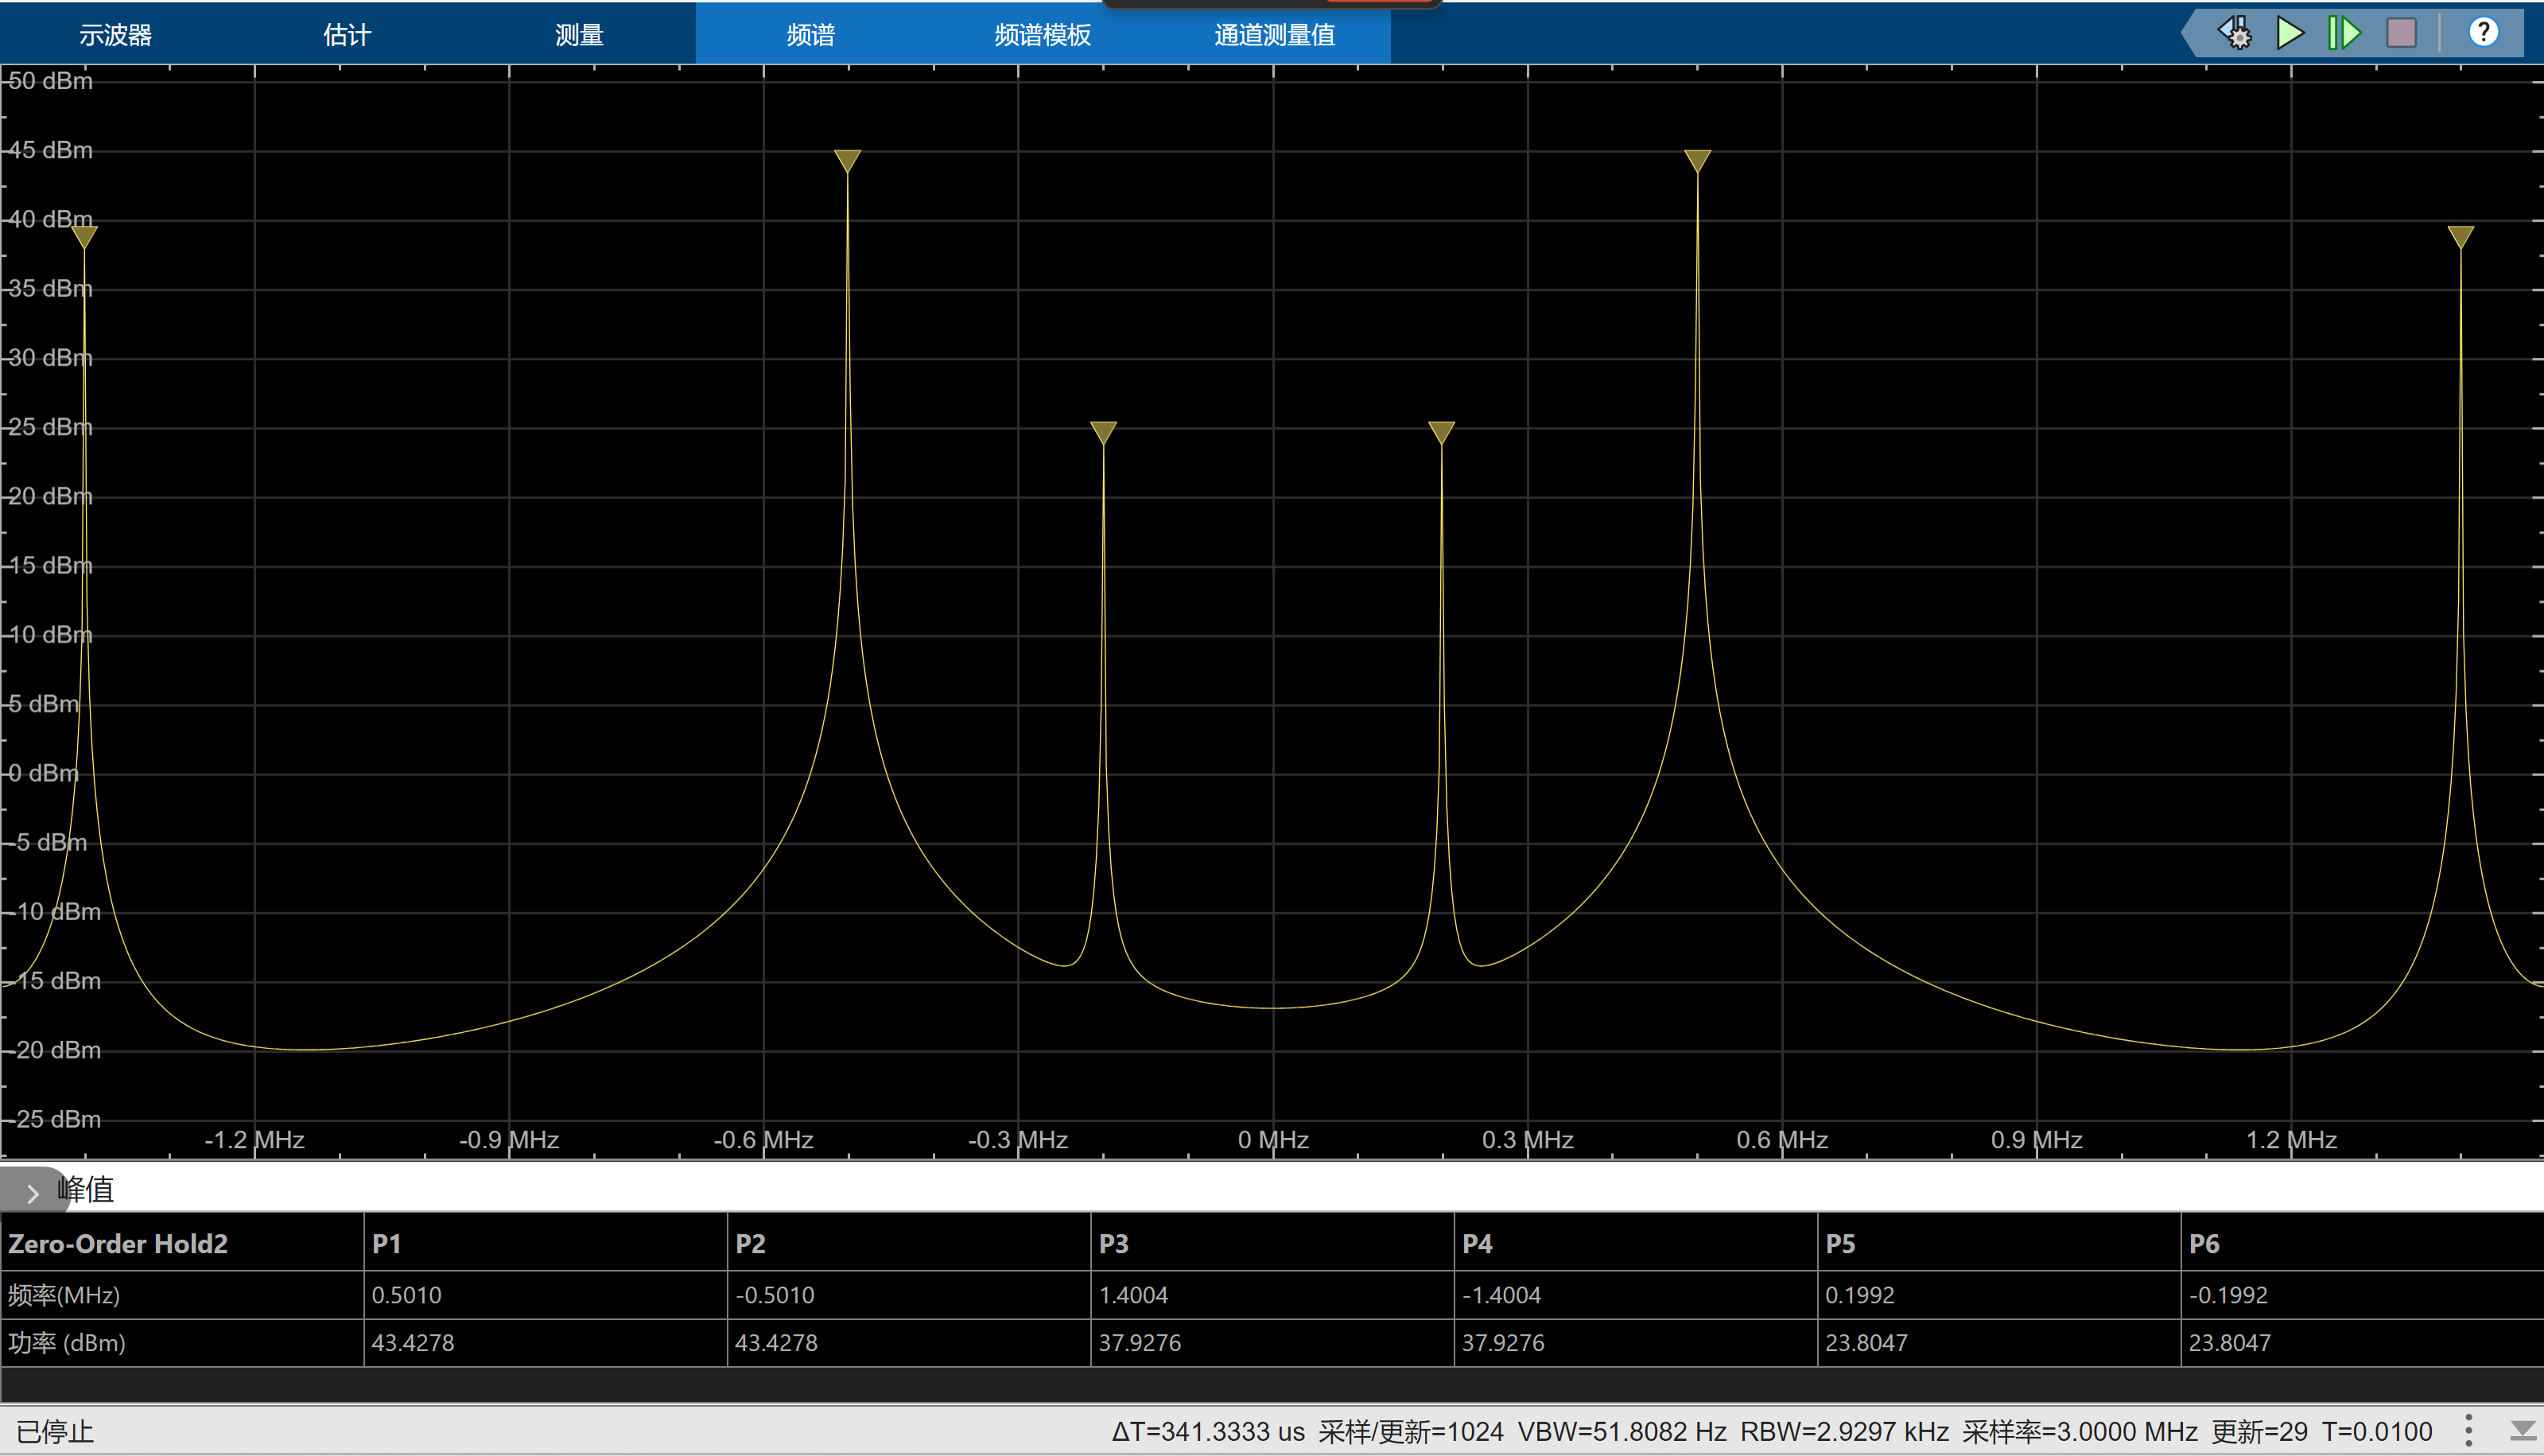
\includegraphics[width=.75\textwidth]{figure/exp1/3M.png}
  \caption{采样频率为3MHz下的输出频谱}
  \label{fig:spectrum3}
\end{figure}
\subsection{基于 MATLAB 的信号采样频谱绘制}
这一部分的实验内容来自《数字信号处理》教材,列举如下。接下来将给出MATLAB代码以及仿真结果。

\begin{example}[一信号是三个正弦信号(频率为50 Hz、500 Hz、1 000 Hz)的和,以8 kHz采样,用适当数量样本画出该信号。]
  \begin{lstlisting}[language=matlab]
fs = 8000; % Sampling frequency, 8 kHz
t = 0:1/fs:1; % Generate time axis, 1 second
f1 = 50;    % First sine wave frequency 50 Hz
f2 = 500;   % Second sine wave frequency 500 Hz
f3 = 1000;  % Third sine wave frequency 1000 Hz

% Signal generation
signal = sin(2*pi*f1*t) + sin(2*pi*f2*t) + sin(2*pi*f3*t);

% Plot time-domain signal
figure;
subplot(2,1,1); % Divide the figure into two parts
plot(t, signal);
title('Time-Domain Signal');
xlabel('Time (seconds)');
ylabel('Amplitude');
grid on;

% Compute and plot spectrum
N = length(signal); % Signal length
fft_signal = fft(signal); % Compute FFT
f = (0:N-1)*(fs/N); % Frequency axis

% Plot only the positive frequency part
half_N = ceil(N/2);
fft_signal = fft_signal(1:half_N);
f = f(1:half_N);

% Compute magnitude spectrum
magnitude = abs(fft_signal)/N;

subplot(2,1,2); % Plot spectrum in the second part of the figure
plot(f, magnitude);
title('Signal Spectrum');
xlabel('Frequency (Hz)');
ylabel('Magnitude');
grid on;

  \end{lstlisting}
\end{example}
仿真结果如图~\ref{fig:fig1}~所示。可以看到频谱在50Hz、500Hz、1000Hz三处分别有一根谱线,这是正弦波的傅里叶变换特性,也证明了频谱分析的意义。
\begin{figure}[htbp]
  \centering
  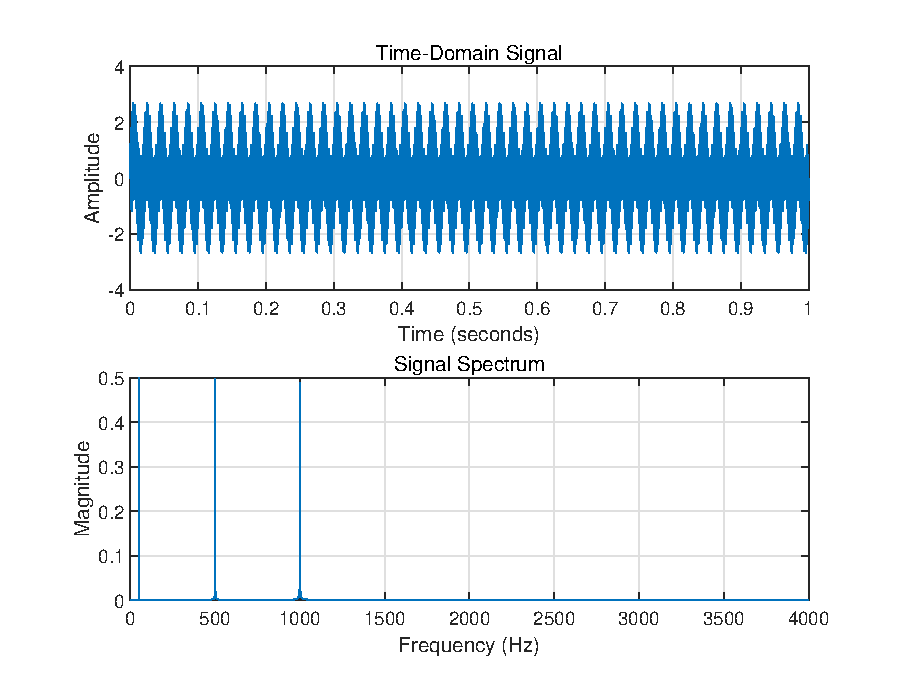
\includegraphics[width=0.65\textwidth]{figure/exp1/fig1.eps}
  \caption{8000Hz采样后的时域频域谱}
  \label{fig:fig1}
\end{figure}
\newpage
\begin{example}[一信号是三个正弦信号(频率为50 Hz、500 Hz、1 000 Hz)的和,以800 Hz采样,用适当数量样本画出该信号,并讨论信号的混叠状况。]
  \begin{lstlisting}[language=matlab]
fs = 800;  % Sampling frequency, 800 Hz
t = 0:1/fs:1; % Generate time axis, 1 second
f1 = 50;    % First sine wave frequency 50 Hz
f2 = 500;   % Second sine wave frequency 500 Hz
f3 = 1000;  % Third sine wave frequency 1000 Hz

% Signal generation
signal = sin(2*pi*f1*t) + sin(2*pi*f2*t) + sin(2*pi*f3*t);

% Plot time-domain signal
figure;
subplot(2,1,1); % Divide the figure into two parts
plot(t, signal);
title('Time-Domain Signal');
xlabel('Time (seconds)');
ylabel('Amplitude');
grid on;

% Compute and plot spectrum
N = length(signal); % Signal length
fft_signal = fft(signal); % Compute FFT
f = (0:N-1)*(fs/N); % Frequency axis

% Compute magnitude spectrum
magnitude = abs(fft_signal)/N;

% Expand frequency range for better visualization
subplot(2,1,2);
plot(f, magnitude);
xlim([0, 1200]); % Set frequency range display from 0 to 1200 Hz
title('Signal Spectrum');
xlabel('Frequency (Hz)');
ylabel('Magnitude');
grid on;

  \end{lstlisting}
\end{example}
仿真结果如图~\ref{fig:fig2}~所示。可以发现,此时的时域谱发生了交叠(闪电型谱线),频域中出现频谱泄露。下面对每条谱线的成因进行分析:
\begin{itemize}
  \item 50Hz:采样前已有频率。
  \item 200Hz:1000Hz频率折叠导致。
  \item 300Hz:500Hz频率折叠导致。
  \item 500Hz:采样前已有频率。
  \item 600Hz:FFT运算带来的1000Hz频率镜像。
  \item 750Hz:50Hz频率折叠。
\end{itemize}
\begin{remark}
该采样不是欠采样,无法重建原有信号。
\end{remark}
\begin{figure}[htbp]
  \centering
  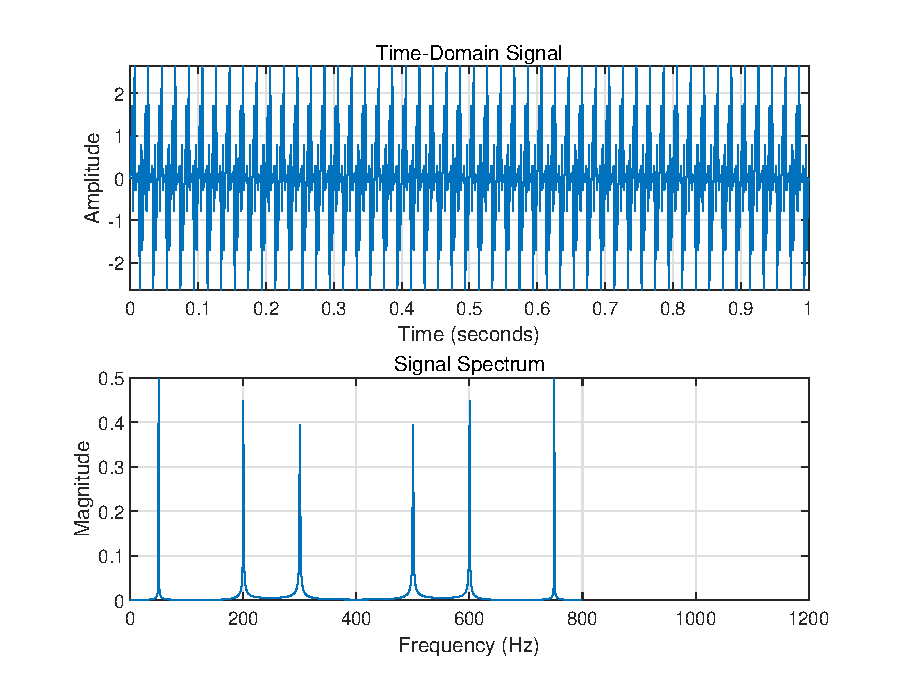
\includegraphics[width=0.65\textwidth]{figure/exp1/fig2.eps}
  \caption{800Hz采样后的时域频域谱}
  \label{fig:fig2}
\end{figure}

\begin{example}[令$x(n) =\cos(2\pi fn/f_s)$,其中$f/f_s$ = 1/16,即每个周期内有16个点。试利用MATLAB编程实现:作M = 4倍的抽取,使每个周期变成4点。作L = 3倍的插值,使每个周期变成48点。
  ]
  \begin{lstlisting}[language=matlab]
f = 1;          % Frequency (Hz)
fs = 16;        % Sampling frequency (Hz)
N = 100;        % Signal length

n = 0:N-1;      % Time sequence
x = cos(2*pi*f*n/fs);  % Original signal

% Perform M = 4 times decimation
M = 4;
x_decimated = decimate(x, M);   % Decimate the signal using the decimate function

% Perform L = 3 times interpolation
L = 3;
x_interpolated = interp(x, L);   % Interpolate the signal using the interp function

% Create a figure to display time-domain and frequency-domain plots
figure;

% First row: Time-domain signals
subplot(3,1,1);
stem(n, x); % Original signal
title('Time-Domain Plot of Original Signal x(n)');
xlabel('Sample index n');
ylabel('Amplitude');
grid on
subplot(3,1,2);
stem(x_decimated);  % Decimated signal
title('Time-Domain Plot of M = 4 Times Decimated Signal');
xlabel('Sample index n');
ylabel('Amplitude');
grid on
subplot(3,1,3);
stem(x_interpolated);  % Interpolated signal
title('Time-Domain Plot of L = 3 Times Interpolated Signal');
xlabel('Sample index n');
ylabel('Amplitude');
grid on
figure;
% Second row: Frequency-domain signals
subplot(3,1,1);
% Spectrum of the original signal
f_orig = abs(fft(x));
f_axis = (0:length(f_orig)-1)*(fs/length(f_orig)); % Frequency axis
stem(f_axis, f_orig);
title('Frequency-Domain Plot of Original Signal x(n)');
xlabel('Frequency (Hz)');
ylabel('Magnitude');
grid on
% Spectrum of the decimated signal
f_dec = abs(fft(x_decimated));
f_axis_dec = (0:length(f_dec)-1)*(fs/M)/length(f_dec); % Frequency axis after decimation

subplot(3,1,2);
stem(f_axis_dec, f_dec);
title('Frequency-Domain Plot of M = 4 Times Decimated Signal');
xlabel('Frequency (Hz)');
ylabel('Magnitude');
grid on
% Spectrum of the interpolated signal
f_interp = abs(fft(x_interpolated));
f_axis_interp = (0:length(f_interp)-1)*(fs*L)/length(f_interp); % Frequency axis after interpolation
subplot(3,1,3);
stem(f_axis_interp, f_interp);
title('Frequency-Domain Plot of L = 3 Times Interpolated Signal');
xlabel('Frequency (Hz)');
ylabel('Magnitude');
grid on
  \end{lstlisting}
\end{example}
仿真结果如图~\ref{fig:fig3}~、~\ref{fig:fig4}~所示,经检验发现符合题目要求。
\begin{figure}[htbp]
  \centering
  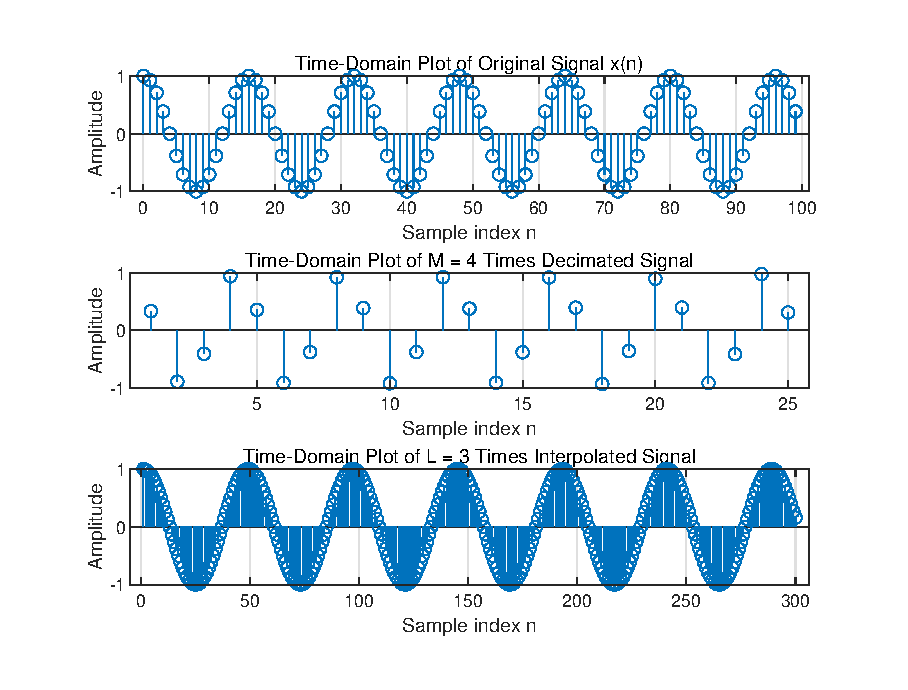
\includegraphics[width=0.65\textwidth]{figure/exp1/fig3.eps}
  \caption{原信号,$M=4$抽取,$L=3$内插后的时域谱}
  \label{fig:fig3}
\end{figure}
\begin{figure}[htbp]
  \centering
  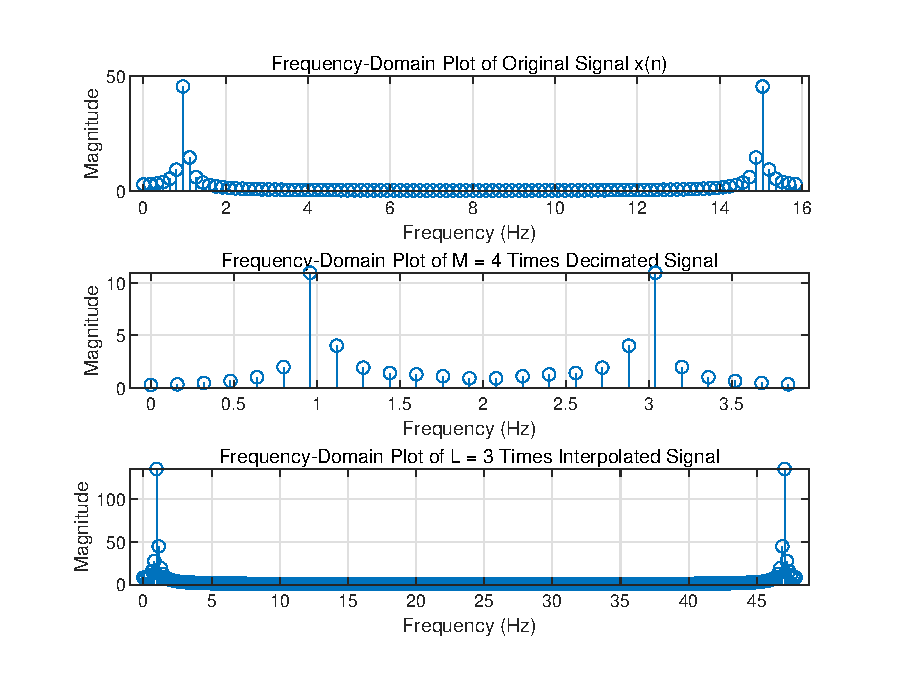
\includegraphics[width=0.65\textwidth]{figure/exp1/fig4.eps}
  \caption{原信号,$M=4$抽取,$L=3$内插后的频域谱}
  \label{fig:fig4}
\end{figure}
\begin{example}[输入信号$x(n)$为归一化频率分别是$f_1$ = 0.04,$f_2$= 0.3的正弦信号相加而成,$N$ = 50,内插因子$L$为5,抽取因子$M$为3,给出按有理因子5/3作采样率转换的输入输出波形。]
  \begin{lstlisting}[language=matlab]
f1 = 0.04;        % Normalized frequency f1
f2 = 0.3;         % Normalized frequency f2
N = 50;           % Signal length

n = 0:N-1;        % Time sequence
x1 = sin(2*pi*f1*n);  % First sine wave
x2 = sin(2*pi*f2*n);  % Second sine wave

% Generate the input signal
x = x1 + x2;

% Set interpolation and decimation factors
L = 5;    % Interpolation factor
M = 3;    % Decimation factor

% Perform sampling rate conversion with a rational factor of 5/3
x_resampled = resample(x, L, M);  % Use the resample function

% Create a figure to display time-domain and frequency-domain plots
figure;

% First row: Time-domain signals
subplot(2,1,1);
stem(n, x); % Input signal
title('Original Signal');
xlabel('n');
ylabel('Amplitude');
grid on
subplot(2,1,2);
stem(x_resampled);  % Resampled signal
title('Resampled Signal');
xlabel('n');
ylabel('Amplitude');
grid on
figure;
% Second row: Frequency-domain signals
subplot(2,1,1);
% Spectrum of the input signal
f_orig = abs(fft(x));
f_axis = (0:length(f_orig)-1)*(1/N); % Normalized frequency
stem(f_axis, f_orig);
title('Frequency Characteristics of Original Signal');
xlabel('Frequency (Hz)');
ylabel('Magnitude');
grid on
subplot(2,1,2);
% Spectrum of the resampled signal
f_resampled = abs(fft(x_resampled));
f_axis_resampled = (0:length(f_resampled)-1)*(1/length(x_resampled)); % Normalized frequency
stem(f_axis_resampled, f_resampled);
title('Frequency Characteristics of Resampled Signal');
xlabel('Frequency (Hz)');
ylabel('Magnitude');
grid on
  \end{lstlisting}
\end{example}
仿真结果如图~\ref{fig:fig5}~、~\ref{fig:fig6}~所示。经检验发现符合题目要求。
\begin{figure}[htbp]
  \centering
  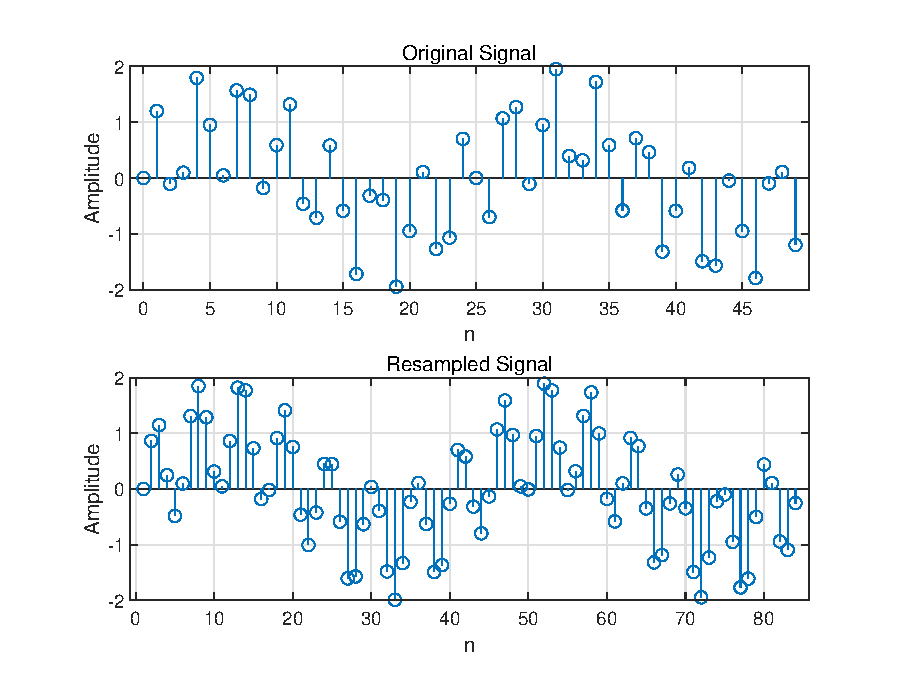
\includegraphics[width=0.65\textwidth]{figure/exp1/fig5.eps}
  \caption{5/3采样率转换后的时域谱}
  \label{fig:fig5}
\end{figure}

\begin{figure}[htbp]
  \centering
  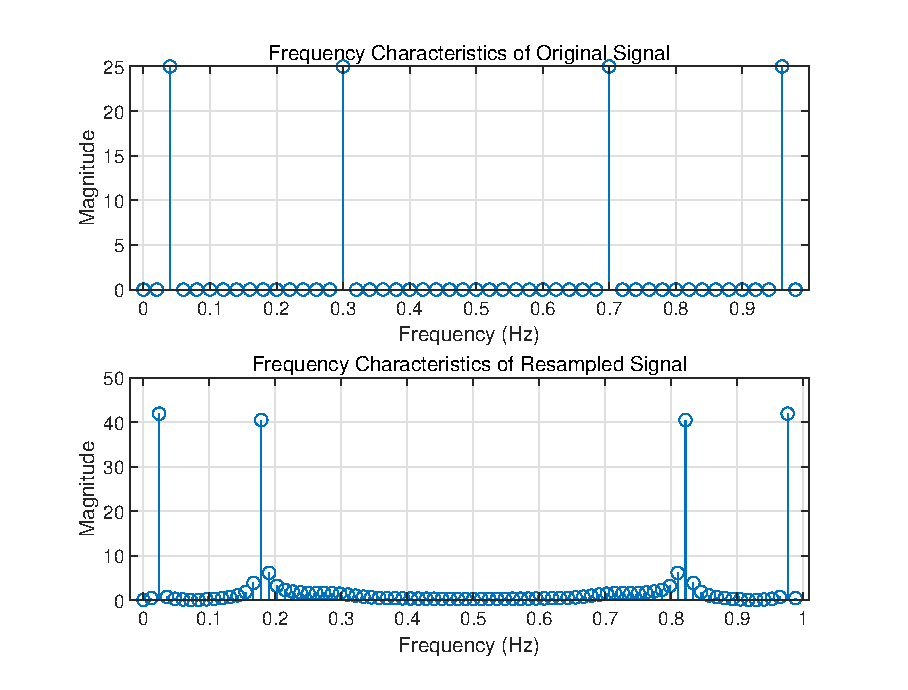
\includegraphics[width=0.65\textwidth]{figure/exp1/fig6.eps}
  \caption{5/3采样率转换后的频域谱}
  \label{fig:fig6}
\end{figure}

% \chapter{FPGA的数字运算}
\begin{introduction}
  \item 有符号数、无符号数的四则运算\textit{Verilog}仿真
  \item \textit{N-bit} 系数量化下系统频率响应\textit{MATLAB}仿真
  \item 有限字长效应的\textit{MATLAB}仿真
\end{introduction}
\section{实验背景和目的}

在数字信号处理系统中,定点数表示和量化误差是非常关键的问题,尤其在进行信号运算和滤波器设计时。随着数字系统的普及,定点数逐渐成为实现高效计算的重要工具。定点数的有限字长效应可能导致数值精度损失,进而影响系统的性能和输出结果。因此,研究定点数在数字运算中的应用,尤其是在滤波器系数量化过程中的影响,具有重要的理论和实践意义。

本实验的目的在于深入探讨数字运算中的定点数表示,研究不同量化方式(如截断与舍入)对系统频率响应的影响,以及有限字长效应如何在实际应用中造成量化误差。通过对定点数和量化误差的理论分析与实验验证,进一步加深对数字信号处理系统的理解,提升对量化与误差控制技术的实际应用能力。

通过本实验,学生将掌握定点数运算的基本原理,理解量化过程中的误差产生机制,并能够在不同量化位宽下评估系统性能。同时,实验也为后续的滤波器设计与系统优化提供了基础,帮助学生更好地应对数字信号处理中常见的精度限制问题。
\section{实验原理}
\subsection{数字运算中使用的定点数}
一般而言,为了硬件存储的方便,数字运算中采用定点数进行运算。尤其是在通信系统中,大多采用不超过16比特的二进制定点数进行数据的存储。\footnote{浮点数也是常用的存储方式,但和本实验关联不大,故不具体叙述。}
在定点数表示中,常见的符号表示方法包括原码、补码和反码。

\textbf{原码}是一种最直观的符号数表示方法,最高位用于表示符号,剩余位数表示数值的绝对值。当符号位为0时,表示正数;当符号位为1时,表示负数。例如,假设采用8比特表示整数:
\[
+5 \Rightarrow 00000101
\]
\[
-5 \Rightarrow 10000101
\]
原码的主要缺点是存在两个零的表示,即 \(+0 = 00000000\) 和 \(-0 = 10000000\),这在运算过程中会导致额外的复杂性。


\textbf{反码}的表示方法是:正数的表示与原码相同,而负数的表示方式是对其对应的正数按位取反(即0变1,1变0)。例如:
\[
+5 \Rightarrow 00000101
\]
\[
-5 \Rightarrow 11111010
\]
反码的优点是加法运算可以直接进行,但仍然存在两个零的表示,即 \(+0 = 00000000\) 和 \(-0 = 11111111\)。


上面两种表示方式各有缺点,因此\textbf{补码}是计算机系统中最常用的定点数表示方法。正数的表示与原码相同,而负数的补码表示是对其对应正数的反码加1。例如:
\[
+5 \Rightarrow 00000101
\]
\[
-5 \Rightarrow 11111011
\]
补码的最大优点在于加法运算可以直接进行,无需额外的进位处理,同时消除了反码中的双零问题,使得只有 \(00000000\) 表示零。此外,补码还能使符号位与数值部分一起参与运算,从而简化了电路实现。

在通信系统、信号处理以及硬件实现中,补码由于其高效性和简化运算的特性,被广泛应用于定点数运算。
\subsection{系数量化造成有限字长效应}
一般而言,为了硬件存储的方便,数字信号处理器(DSP)中通常采用有限精度的定点数进行运算。然而,由于有限精度表示,滤波器系数在量化后会引入误差,这种误差对系统性能的影响称为系数量化效应。

在实际DSP实现中,滤波器的系数也需要用有限比特宽度的定点数或浮点数进行表示。当理想滤波器系数 \( h[n] \) 量化为有限比特宽度的表示 \( \hat{h}[n] \) 时,会引入量化误差:
\begin{equation}
e[n] = h[n] - \hat{h}[n]
\end{equation}
这种误差会导致滤波器的幅频响应和相频响应偏离理想情况,并可能引入额外的增益或相位畸变。


对于无限脉冲响应(IIR)滤波器,系数量化误差可能导致极点的位置发生偏移,进而影响系统的稳定性。当极点位于单位圆外时,滤波器就会不稳定。因此,在IIR滤波器设计中,需要特别关注系数量化对极点分布的影响,并可采用高精度系数或级联结构来减小量化误差的影响。


对于有限脉冲响应(FIR)滤波器,系数量化主要影响滤波器的频率响应,导致幅频特性偏差。然而,由于FIR滤波器没有极点,因此量化不会影响系统的稳定性。为了减小量化误差,可以采用较高比特宽度的系数表示,或者利用最佳逼近方法来优化量化方案。

为了减小系数量化效应,通常采用以下几种方法:
\begin{itemize}
    \item \textbf{增加比特宽度}:提高系数的表示精度,以降低量化误差。
    \item \textbf{采用级联结构}:在IIR滤波器中,使用级联二阶节(biquad structure)可以减小极点的偏移,提高系统稳定性。
    \item \textbf{最小化量化误差}:采用最佳逼近方法,如均方误差(MSE)优化或其他优化算法,使量化误差最小化。
    \item \textbf{过采样}:通过提高采样率,使量化噪声的影响分布在更宽的频带范围内,然后利用抗锯齿滤波减少有害影响。
\end{itemize}

在DSP系统设计中,系数量化效应是不可避免的,但通过合理的设计策略,可以有效降低其对系统性能的影响。
\subsection{A/D量化器中产生的量化噪声}
在数字信号处理中,模拟信号需要经过模数转换(A/D转换)才能在数字系统中进行处理。然而,由于A/D转换器的有限分辨率,输入信号在量化过程中会产生量化误差,这种误差表现为量化噪声,并影响信号质量。为了衡量量化噪声对信号的影响,通常采用量化信噪比(SQNR, Signal-to-Quantization-Noise Ratio)来评估系统性能。


在A/D转换过程中,模拟信号 \( x(t) \) 经过取样后得到离散信号 \( x[n] \),然后被映射到有限比特数的数字表示 \( \hat{x}[n] \),通常假设产生的量化误差分布均匀且在\([- \Delta /2, \Delta /2]\) 之间,其中 \( \Delta \) 为量化步长。若信号的量化误差服从均匀分布,则可以计算其均方误差(即量化噪声的功率):
\begin{equation}
  \sigma_q^2 = \frac{\Delta^2}{12}
\end{equation}


其中,量化步长 \( \Delta \) 由ADC的分辨率 \( B \) 和满量程范围 \( V_{\max} - V_{\min} \) 确定:
\begin{equation}
  \Delta = \frac{V_{\max} - V_{\min}}{2^B}
\end{equation}


\textbf{量化信噪比}(SQNR,Signal-to-Quantization-Noise Ratio)定义为信号的均方值与量化噪声功率的比值,通常采用分贝(dB)表示:
\[
\text{SQNR} = 10 \log_{10} \left( \frac{\sigma_x^2}{\sigma_q^2} \right)
\]
假设输入信号为均匀分布或满幅正弦波,其均方值可表示为:
\[
\sigma_x^2 = \frac{(V_{\max} - V_{\min})^2}{12}
\]
代入量化噪声功率 \(\sigma_q^2\) 后,可以得到SQNR的表达式:
\[
\text{SQNR} = 6.02B + 1.76 \quad \text{(dB)}
\]
从该公式可以看出,A/D转换器的分辨率 \( B \) 每增加1比特,SQNR约提升 6.02 dB。

为了减小量化噪声,提高系统的量化信噪比,可以采用以下几种方法:
\begin{itemize}
    \item \textbf{增加ADC的位数}:提高量化分辨率 \( B \),从而减小量化误差,提高SQNR。
    \item \textbf{增大输入信号幅度}:适当调整输入信号的动态范围,使其接近ADC的满量程范围,从而充分利用量化级数,提高信号能量。
    \item \textbf{过采样}:通过提高采样率,将量化噪声的频谱展宽,然后利用抗锯齿滤波减少有害噪声,等效提高SQNR。
    \item \textbf{采用噪声整形技术}:在高阶A/D转换器(如Sigma-Delta ADC)中,利用反馈结构将量化噪声移出信号带宽,提高信号质量。
\end{itemize}

在数字信号处理和通信系统中,量化噪声是不可避免的,但通过优化ADC设计和信号处理策略,可以有效降低其影响,提高系统性能。在本次实验中,我们重点讨论 N-bit 系数量化下系统频率响应以及运算有限字长效应对滤波器输出响应的影响。

\section{实验使用软件}
\begin{itemize}
  \item Visual Studio Code,用于Verilog 文件的撰写;
  \item iverilog,用于Verilog编译;
  \item gtkwave,用于波形显示。
  \item MATLAB R2024b,用于系数量化和有限字长效应实验。
\end{itemize}
\section{实验内容}
\subsection{有符号数、无符号数的四则运算Verilog仿真}
在数字电路设计中,处理有符号数与无符号数的运算是基础且关键的任务。由于计算机通常采用补码表示有符号数,因此在进行加、减、乘、除等四则运算时,必须特别注意符号扩展和进位处理。本实验通过 Verilog 编写四则运算模块,分别实现有符号数和无符号数的计算,并通过仿真验证其正确性。
\subsubsection{模块外部接口定义}
为了模块更利于用户理解,四则运算使用相同名称的I/O接口,列举如表~\ref{table:interface}~。
\begin{table}[htbp]
    \centering
    \begin{tabular}{ccc}
      \toprule
       信号名 & 意义 & 端口类型\\
      \midrule
        \texttt{i\_a} & 运算模块的第一个输入 & Input \\
       \texttt{i\_b} & 运算模块的第二个输入 & Input \\
       \texttt{signed\_result} & 有符号数输出 & Output \\
       \texttt{unsigned\_result} & 无符号数输出 & Output \\
      \bottomrule
    \end{tabular}
    \caption{运算模块接口说明}
    \label{table:interface}
\end{table}
\subsubsection{模块功能说明}
以\textbf{ADD}模块为例,说明模块的功能。ADD模块的代码如下所示。
\begin{lstlisting}[language=verilog]
  module ADD(
    input [3:0] i_a,
    input [3:0] i_b,
    output [4:0] o_unsigned_result,
    output [4:0] o_signed_result
);

wire signed [3:0] signed_a;
wire signed [3:0] signed_b;

assign signed_a = i_a;
assign signed_b = i_b;
assign o_unsigned_result = i_a + i_b;
assign o_signed_result = signed_a + signed_b;

endmodule
\end{lstlisting}

如代码所示,它实现了位宽为4的信号\texttt{i\_a}和\texttt{i\_b}作为无符号数或有符号数的相加,结果预留一位作为最高位进位的存储。其它三种运算类似\texttt{ADD}模块的写法,此处不再赘述。
\subsubsection{模块测试}
以\textbf{ADD}模块的测试为例,其余三个模块类似该模块的测试。将所有输入可能性写入Test case,编写 Verilog Testbench如下:
\begin{lstlisting}{language=verilog}
  `timescale 1ns/1ps

module tb_ADD;

    reg [3:0] a;
    reg [3:0] b;
    wire [4:0] signed_result;
    wire [4:0] unsigned_result;

    ADD dut(
        .i_a(a),
        .i_b(b),
        .o_signed_result(signed_result),
        .o_unsigned_result(unsigned_result)
    );
    integer i, j;

    initial begin
        a = 4'd0; b = 4'd0; #10;
        a = 4'd0; b = 4'd1; #10;
        a = 4'd0; b = 4'd2; #10;
        // ...
        a = 4'd0; b = 4'd14; #10;
        a = 4'd0; b = 4'd15; #10;
        // ...

        a = 4'd15; b = 4'd10; #10;
        a = 4'd15; b = 4'd11; #10;
        a = 4'd15; b = 4'd12; #10;
        a = 4'd15; b = 4'd13; #10;
        a = 4'd15; b = 4'd14; #10;
        a = 4'd15; b = 4'd15; #10;
    #1000 $finish;
    end

    initial begin
        $dumpfile("add.vcd");
        $dumpvars(0,tb_ADD);
    end
endmodule
\end{lstlisting}
用iverilog编译器编译待测模块和Testbench,得到仿真波形文件(vcd格式),之后使用轻量级波形预览软件GTKwave进行波形预览,得到四则运算的测试波形图如图~\ref{fig:verilog_test}~。\footnote{为了符合四则运算的直观认识,对于有符号数部分的输入输出,采用了\texttt{signed\_decimal}格式,而对无符号数部分采用了\texttt{decimal}格式。}
\begin{figure}[htbp]
  \centering
  \subfloat[\texttt{ADD}模块部分测试数据]{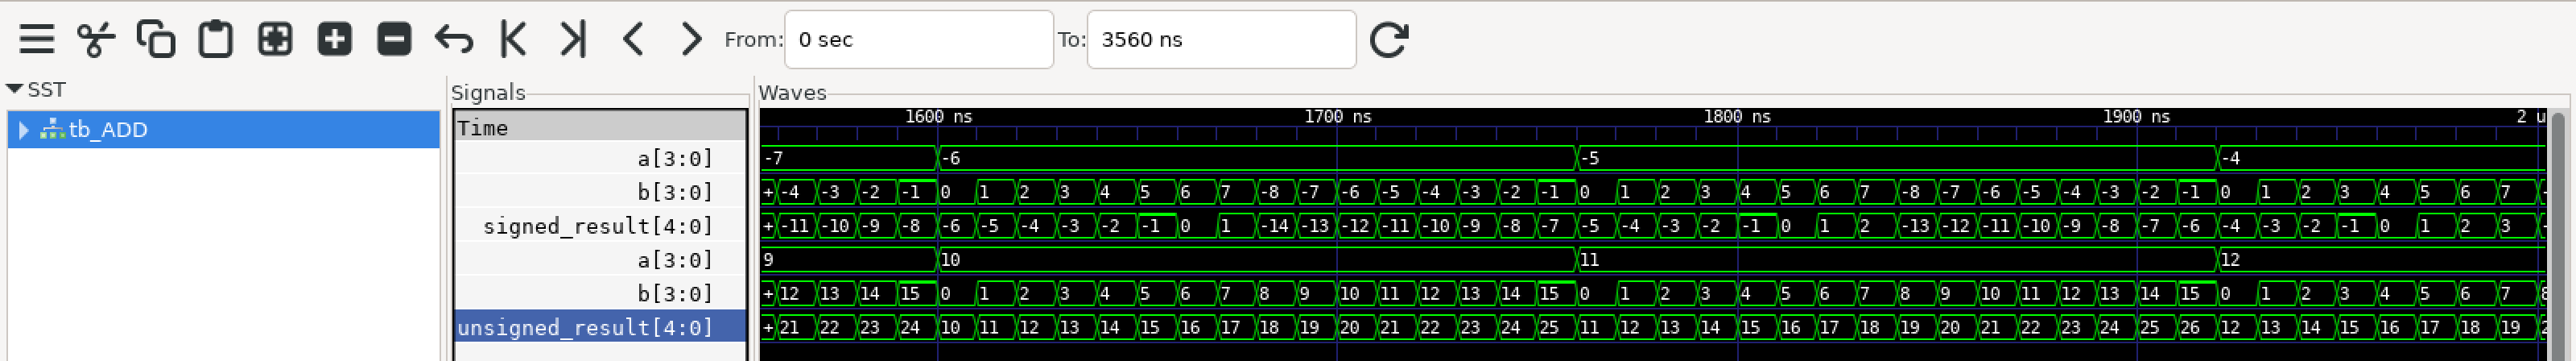
\includegraphics[width=0.95\textwidth]{figure/exp2/wave_add.png}}
  \newline
  \subfloat[\texttt{SUB}模块部分测试数据]{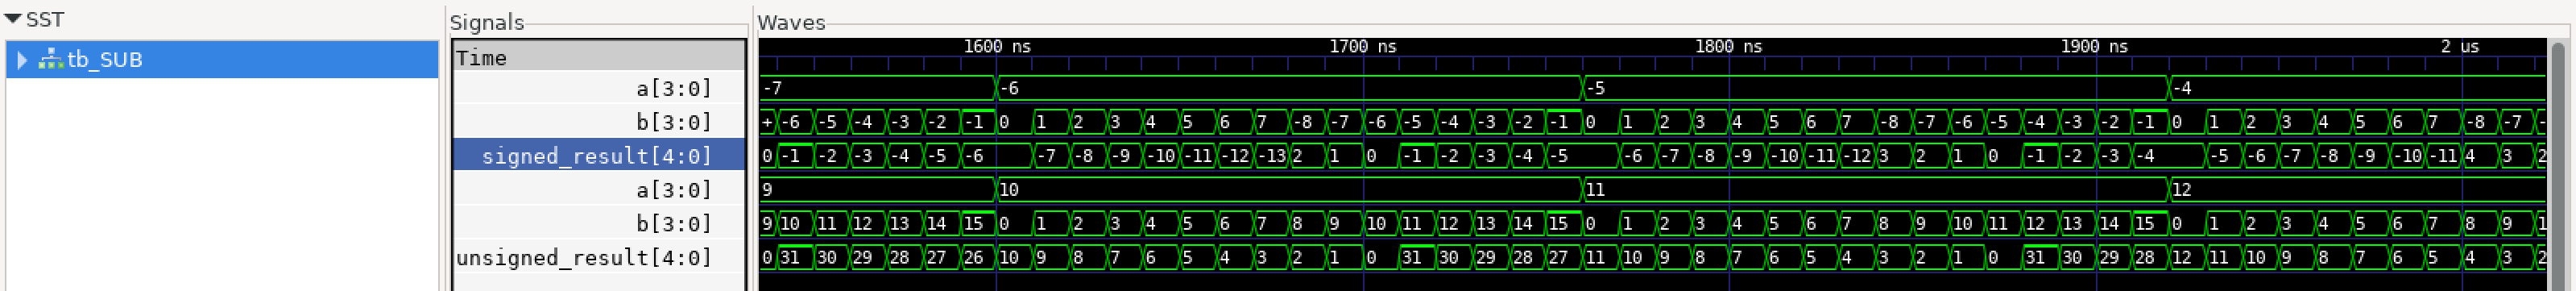
\includegraphics[width=0.95\textwidth]{figure/exp2/wave_sub.png}}
  \newline
  \subfloat[\texttt{MUL}模块部分测试数据]{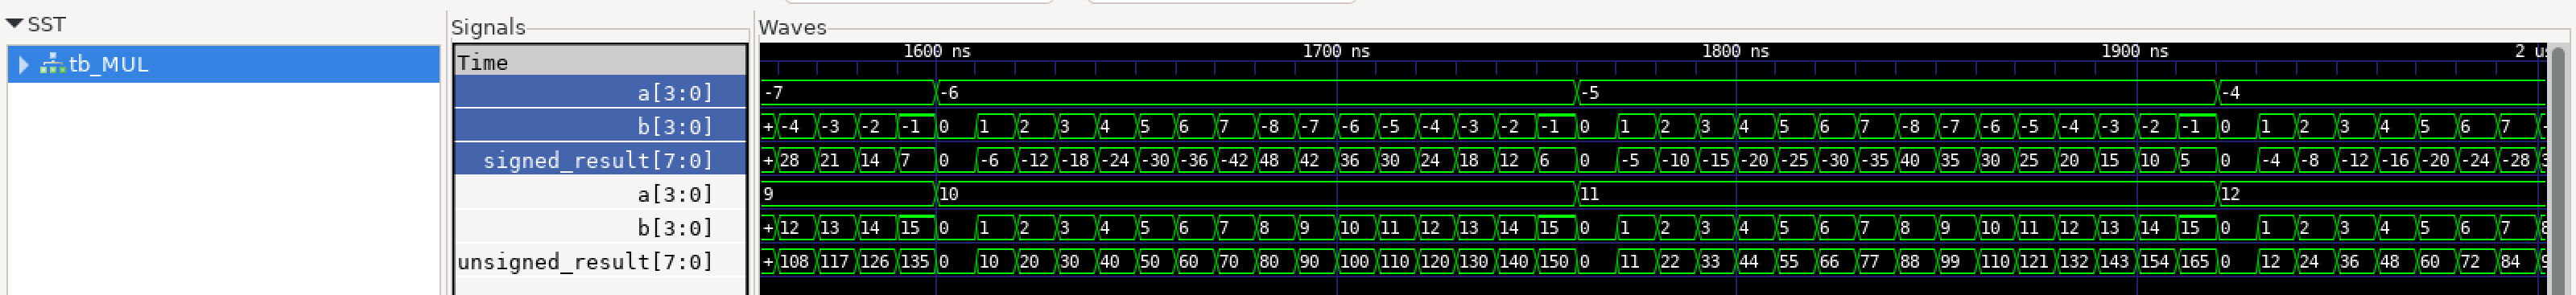
\includegraphics[width=0.95\textwidth]{figure/exp2/wave_mul.png}}
  \newline
  \subfloat[\texttt{DIV}模块部分测试数据]{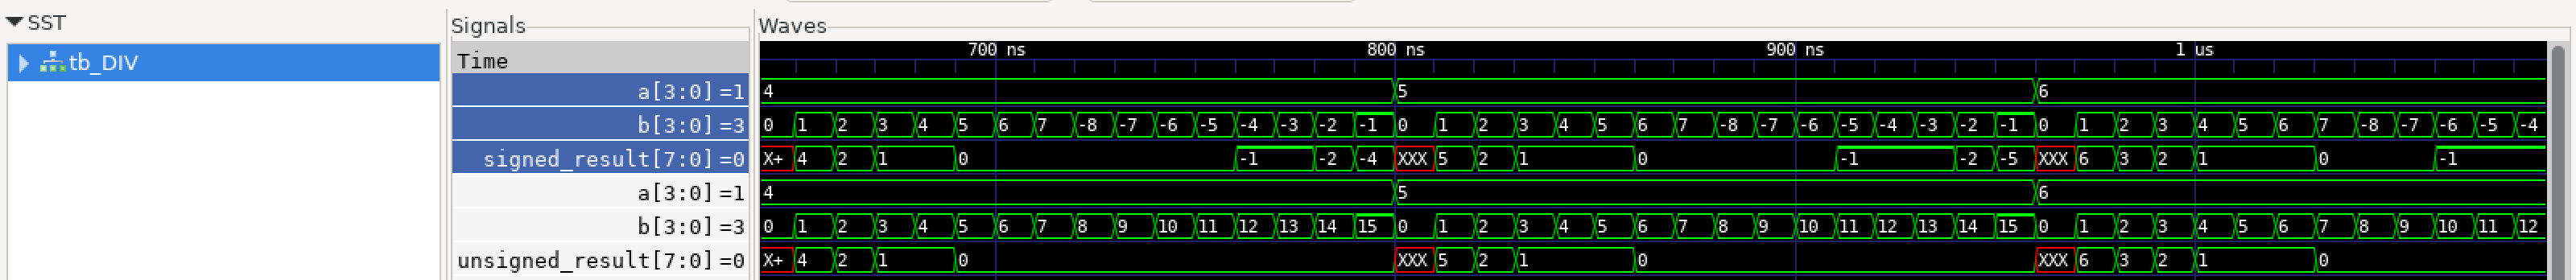
\includegraphics[width=0.95\textwidth]{figure/exp2/wave_div.png}}
  \caption{有符号数、无符号数四则运算Verilog仿真的部分测试数据}
  \label{fig:verilog_test}
\end{figure}

可以看到,对于加、减、乘三种运算,仿真结果均显示了正确的结果,没有溢出现象的发生。对于除运算,输出结果为向下取整。当除数为0时,输出结果为“X”(即不确定),这也符合预期。  

\subsection{N-bit 滤波器系数量化下系统频率响应MATLAB仿真}
构建一个IIR滤波器,其系统函数为:
\begin{equation}
  H(z) = \frac{0.05}{1+1.7z^{-1}+0.745z^{-2}}
\end{equation}
教材中已给出8-bit系数量化效应下系统单位脉冲频率响应与无限精度的系统频率响应的对比。结果表明:有限精度下系统的频率响应幅度会下降。为了进一步探究这种频率响应的变化原因,更改量化位宽后重新进行仿真。选择量化位宽为10-bit,6-bit,4-bit,量化方式为\texttt{round}(四舍五入),将单位脉冲序列为输入时的频率响应与原系统频率响应进行比较。编写MATLAB代码如下。


\begin{lstlisting}{language=matlab}
b = 0.05;
a = [1, 1.7, 0.745];

% 归一化
max_a_b = max(max(b), max(a));
b1 = b / max_a_b;
a1 = a / max_a_b;

% 量化位数
Q = [10, 6, 4];

% 计算量化系数
scale_factors = 2.^(Q - 1) - 1;
b_quant = round(b1 * scale_factors);
a_quant = round(a1' * scale_factors); 

% 生成脉冲输入
N = 2048;
xn = (0:N-1) / N * 2;
dn = [1, zeros(1, N-1)];

% 计算原系统的频率响应
hn = filter(b, a, dn);
fn = 10 * log10(abs(fft(hn, N)));
fn = fn - max(fn); % 归一化

% 绘制原系统的频率响应
figure;

plot(xn(1:N/2), fn(1:N/2), '-k', 'LineWidth', 1.5);
hold on;
legend_entries = ["原系统的频率响应"];

% 计算量化后的频率响应
for i = 1:length(Q)
    hn_quant = filter(b_quant(i), a_quant(:,i)', dn);
    fn_quant = 10 * log10(abs(fft(hn_quant, N)));
    fn_quant = fn_quant - max(fn_quant);
    % 绘制量化后的频率响应
    plot(xn(1:N/2), fn_quant(1:N/2), '--', 'LineWidth', 1.2);
    legend_entries = [legend_entries, sprintf('%d 比特量化后的频率响应', Q(i))];
    
    % 计算并输出量化系统的极点
    s_quant = roots(a_quant(:,i));
    disp(['量化位数 ', num2str(Q(i)), ' 的极点:']);
    disp(s_quant);
end

% 设置图例和坐标轴标签
xlabel('归一化频率(f_s/2)',"Interpreter","tex");
ylabel('归一化幅度(dB)');
legend(legend_entries, 'Location', 'Best');
title("原系统、10比特、6比特、4比特量化位宽量化频率响应");
grid on;
hold off;

\end{lstlisting}

运行该代码,得到舍入方式下的频率响应如图~\ref{fig:RND}~。将该代码中的\texttt{round}替换为\texttt{floor}就可以得到截断方式的仿真结果,如图~\ref{fig:TRN}~所示。
\begin{figure}[htbp]
  \centering
  \subfloat[舍入方式\label{fig:RND}]{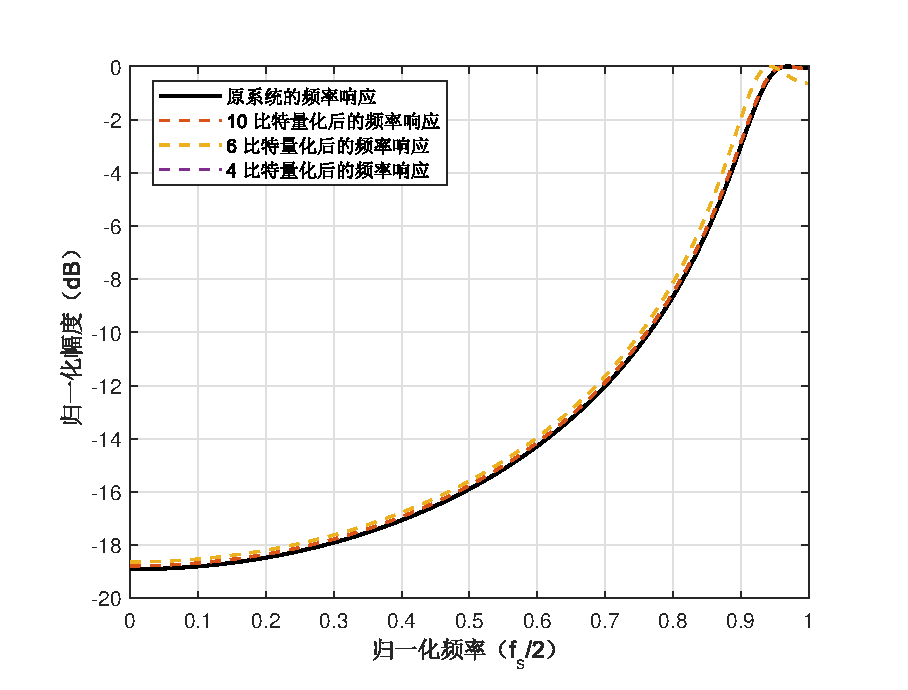
\includegraphics[width=0.45\textwidth]{figure/exp2/2-2round.eps}}
  \hfill
  \subfloat[截断方式\label{fig:TRN}]{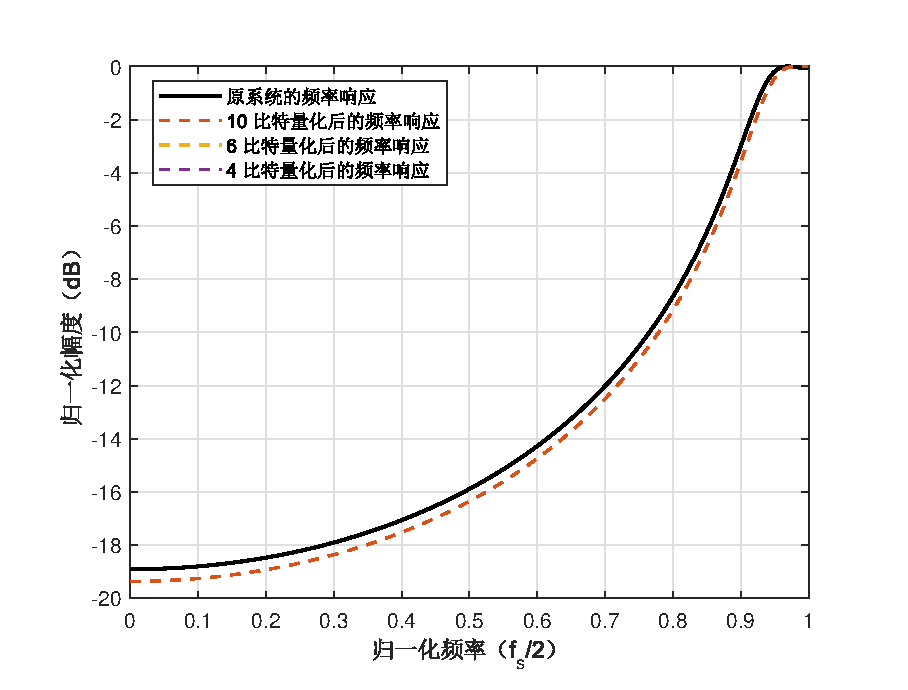
\includegraphics[width = 0.45\textwidth]{figure/exp2/2-2truncate.eps}}
  \caption{原系统,10-bit,6-bit,4-bit系数截断/舍入量化下的系统频率响应}
\end{figure}

可以看到,截断方式下4-bit和6-bit的仿真图线和舍入方式下的4-bit仿真图线都没有正常显示,经过检查发现:此时滤波器的分子系数被量化为0,导致输出响应为0。此时系统的极点也为纯实数。另外,舍入方式下,系统的频率响应随着量化位数的增加而有些许降低;截断方式下,系统的频率响应随着量化位数的增加而有些许上升。这可能是因为舍入方式下系数量化引入了小幅误差,误差随位宽增加逐渐减少,使系统频率响应整体趋向下降。而截断方式下始终往 0 方向偏移,使得系统初始增益降低,随着位宽增加,增益逐渐恢复,导致频率响应上升。\footnote{并不确定这种表述的正确性。}并且,截断方式下,相同量化位数引入的误差大于舍入方式下引入的误差。这是因为舍入方式下系数会朝着更贴近真实系数的方向量化,而截断方式下系数永远会向下量化,从而有更大的可能性获得更大的误差。\footnote{将分子系数换为0.5时,四种仿真图线全能够正常显示,这是因为此时滤波器系数的分子会被量化为一个整数而不是0,使得单位脉冲响应作用下的系统频率响应存在。因此可以将滤波器系数同乘一个常数,或提升单位脉冲响应的幅值。}


\subsection{运算有限字长效应的MATLAB仿真}
在系数量化效应的实验中,我们在滤波器系数创建时就将其使用截断或舍入方式量化。而在运算有限字长效应的实验中,我们默认滤波器系数是理想的,并在输出部分加一次舍入量化。令输入$x[n] = \frac{7}{8}\delta(n)$,观察2-bit,4-bit,6-bit量化效应下的输出响应。编写MATLAB代码如下:
\begin{lstlisting}[language=matlab]
clc; clear; close all;

% Input
x = [7/8 zeros(1, 15)];
N = length(x);
y = zeros(1, N);
% Coefficients
A = 0.5;
B_values = [2, 4, 6]; % Data Width
Qy_results = cell(1, length(B_values)); % Storage Init

% Original
for i = 1:N
    if i == 1
        y(i) = x(i);
    else
        y(i) = -A * y(i-1) + x(i);
    end
end
% 需要注意的是,系统在每一次计算出结果时,都会进行一次输出结果量化,因此不能用filter函数进行计算
% Quantized
for b_idx = 1:length(B_values)
    B = B_values(b_idx);
    Qy = zeros(1, N); % 初始化存放量化结果

    for i = 1:N
        if i == 1
            Qy(i) = x(i);
        else
            Qy(i) = -A * Qy(i-1) + x(i);
        end
        % RND
        Qy(i) = round(Qy(i) * (2^(B-1))) / 2^(B-1);
    end
    
    Qy_results{b_idx} = Qy;
end
colors = [0, 0.447, 0.741;  % 亮蓝色
          0.850, 0.325, 0.098;  % 鲜橙色
          0.494, 0.184, 0.556;  % 深紫色
          0.466, 0.674, 0.188]; % 鲜绿色

markers = {'o', 's', 'd', '^'}; % 圆点, 方块, 菱形, 三角形
xa = 0:N-1;
figure; hold on;

plot(xa, y, '-o', 'Color', colors(1, :), 'MarkerFaceColor', colors(1, :), ...
    'LineWidth', 1, 'MarkerSize', 6, 'DisplayName', '原系统运算结果');

for b_idx = 1:length(B_values)
    B = B_values(b_idx);
    Qy = Qy_results{b_idx};
    plot(xa, Qy, '-o', 'Color', colors(b_idx + 1, :), 'MarkerFaceColor', colors(b_idx + 1, :), ...
        'LineWidth', 1, 'Marker', markers{b_idx + 1}, 'MarkerSize', 6, ...
        'DisplayName', sprintf('%d-bit 量化结果', B));
end

legend;
xlabel('运算次数');
ylabel('滤波结果');
grid on;

xlim([-1, N]); % X 轴范围
y_min = min([y, Qy_results{:}]) - 0.1; % 计算所有数据的最小值
y_max = max([y, Qy_results{:}]) + 0.1; % 计算所有数据的最大值
ylim([y_min, y_max]); % 设置 Y 轴范围
\end{lstlisting}

运行该代码,得到原系统与三种量化位宽进行输出结果量化后的结果随运算次数(序列长度)的变化如图~\ref{fig:2-3}~。可以看到,随着运算次数增加,量化后的三条曲线均出现了在两个量化电平间不断切换的现象。

\begin{figure}[htbp]
  \centering
  \begin{minipage}{0.5\linewidth}
    \baselineskip = 1.25 \baselineskip
    一般而言,量化误差的误差来源为以下三种:
    \begin{itemize}
        \item \textbf{舍入误差(Rounding Error)}:由于量化过程中数值需要映射到有限比特位表示的离散值,导致计算结果与理论值之间存在误差。
        \item \textbf{极限环振荡(Limit Cycle Oscillation)}:在反馈系统或 IIR 滤波器中,有限精度计算可能导致信号在若干固定值之间振荡,而无法进一步衰减。
        \item \textbf{量化噪声(Quantization Noise)}:低比特位量化会引入类似噪声的现象,使信号无法平滑下降到零,而是在某个范围内不规则波动。
    \end{itemize}

    通过对比实验数据,我们观察到以下现象:

    \begin{itemize}
        \item 在\textbf{无限精度计算}条件下,信号能平滑衰减至零,符合理论期望。
        \item 在\textbf{有限精度计算}条件下,当信号幅值降低到一定范围时,输出值在某些固定值处振荡,无法继续趋近于零。
        \item \textbf{量化比特位越低},信号的跳变幅度越大,震荡现象越明显。
    \end{itemize}


  \end{minipage}
  \hfill
  \begin{minipage}{0.45\linewidth}
    \centering
    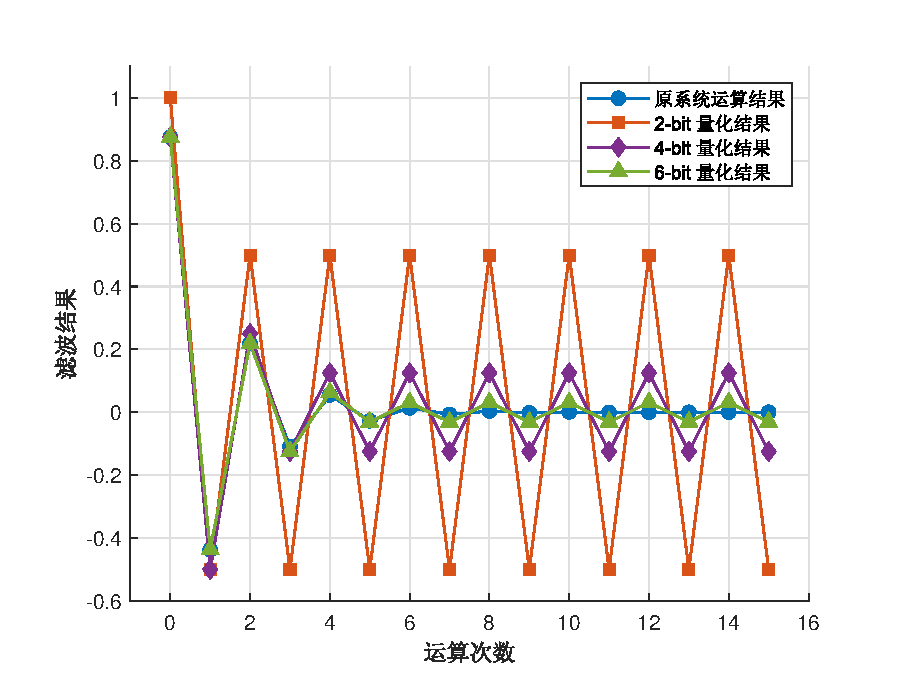
\includegraphics[width=0.95\linewidth]{figure/exp2/2-3.eps}
    \caption{原系统,2-bit,4-bit,6-bit运算量化下输出结果的对比}
    \label{fig:2-3}
  \end{minipage}
\end{figure}

根据本实验的实验结果,推测出现图~\ref{fig:2-3}~中的波形的原因是极限环振荡。



% 
\chapter{Xilinx 7系列FPGA和IP核的使用}
\begin{introduction}
  \item \textit{Clocking Wizard IP Core}的使用
  \item \textit{DDS Compiler IP Core}的使用
  \item \textit{Integrated Logic Analyzer(ILA) IP Core}的使用
  \item 调用\textit{IP}核输出余弦信号到实验平台
\end{introduction}
\section{实验背景与目的}
随着 FPGA(Field Programmable Gate Array)技术的快速发展,基于 FPGA 的数字信号处理、嵌入式系统和高性能计算得到了广泛应用。Xilinx 7 系列 FPGA 作为当前主流的可编程逻辑器件之一,提供了丰富的硬件资源和灵活的开发环境。Vivado 设计套件(Vivado Design Suite)作为 Xilinx 提供的综合开发工具,支持 FPGA 设计、仿真、调试以及 IP 核的集成,极大地提高了开发效率。

在 FPGA 设计过程中,IP(Intellectual Property)核作为一种预先设计好的模块,提供了高效、可靠的硬件功能封装。通过调用 Xilinx 提供的 IP 核,开发者可以快速实现复杂的功能,例如时钟管理(Clocking Wizard)、数字信号处理(DDS Compiler)、片上调试(Integrated Logic Analyzer, ILA)等,从而减少低级电路设计的复杂性,提高开发效率。

本实验通过 Xilinx 7 系列 FPGA 及 Vivado 设计环境,介绍如何使用和配置常见的 IP 核,并结合具体应用场景,实现特定功能,如时钟信号的生成、余弦波信号的合成以及片上逻辑分析等。

\section{实验原理}
\subsection{IP 核}
\begin{definition}[IP核]
  Xilinx 提供了一系列 IP 核(Intellectual Property Cores),这些是可复用的硬件模块,用于加速 FPGA 设计开发。IP 核可以是预先优化的逻辑电路,如 DSP 处理单元、存储接口、AXI 总线接口等。使用 IP 核可以减少设计时间,提高 FPGA 资源利用率,并优化性能。
\end{definition}


Xilinx IP 核主要包括数学计算(DDS Compiler、CORDIC)、信号处理(FIR Compiler、FFT)、存储管理(BRAM Controller、FIFO Generator)、通信接口(AXI Interconnect、UART、SPI)、DSP 加速(DSP Slice、HLS 生成的 IP)、时钟管理(Clocking Wizard、PLL)等类别。

在 Vivado 中,用户可以通过 \texttt{IP Catalog} 选择合适的 IP 核,配置输入/输出接口、数据位宽和时钟频率,并生成 RTL 代码。然后,可以在 Verilog 代码中实例化该 IP 核,例如:
\begin{lstlisting}[language=verilog]
dds_compiler_0 my_dds (
    .aclk(clk), 
    .s_axis_config_tvalid(1'b1),  
    .s_axis_config_tdata(16'H51E), 
    .m_axis_data_tvalid(),   
    .m_axis_data_tdata(sin_out) 
);
\end{lstlisting}

此外,用户可以使用 Xilinx Vitis HLS 通过 C++ 代码生成 IP 核,例如:
\begin{lstlisting}[language=C++]
void my_ip(ap_fixed<16,8> in, ap_fixed<16,8> &out) {
    out = in * 1.5;
}
\end{lstlisting}
然后在 Vivado 中综合并调用。

由于 Icarus Verilog(iverilog)不支持直接仿真 Xilinx IP 核,推荐使用 Vivado 自带的 \texttt{xsim} 进行仿真,或者手写 Verilog 模型替代 IP 核。

综上所述,Xilinx IP 核能够显著加速 FPGA 设计,减少手写代码量,提高设计效率。用户可以根据具体需求选择合适的 IP 核,并结合 HLS 技术优化 FPGA 设计流程。
\subsection{调用 IP 核的一般方法}

在 FPGA 设计中,IP 核的调用通常分为以下几个步骤:IP 选择、参数配置、实例化、综合及仿真。Xilinx 提供的 IP 核可以通过 Vivado 进行管理,用户可以根据需要调用适当的 IP 核,提高开发效率。

首先,在 Vivado 中打开 \texttt{IP Catalog},搜索所需的 IP 核,例如 \texttt{DDS Compiler} 生成余弦波,\texttt{FIFO Generator} 用于数据缓存,\texttt{AXI Interconnect} 用于总线连接等。用户可以双击 IP 核进入配置界面,调整数据位宽、时钟频率、接口类型等参数。

配置完成后,点击 \texttt{Generate} 生成相应的 RTL 代码和示例文件。生成的文件通常包括 HDL 代码、仿真模型和 IP 的 \texttt{xci} 配置文件。在 Verilog 或 VHDL 代码中,用户需要实例化该 IP 核,例如对一个FIFO模块的例化:
\begin{lstlisting}[language=verilog]
fifo_generator_0 my_fifo (
    .clk(clk),
    .srst(reset),
    .din(data_in),
    .wr_en(write_enable),
    .rd_en(read_enable),
    .dout(data_out),
    .full(full),
    .empty(empty)
);
\end{lstlisting}

综合(Synthesis)和实现(Implementation)完成后,可以使用 \texttt{xsim} 进行仿真,或者直接下载到 FPGA 进行调试。如果需要与上层软件交互,可以通过 \texttt{AXI} 接口连接处理器(如 MicroBlaze 或 ARM 核),并在 Vitis 软件环境中编写驱动代码。例如,使用 Xilinx 提供的 API 访问 FIFO:
\begin{lstlisting}[language=C++]
Xil_Out32(FIFO_BASEADDR, data);
data = Xil_In32(FIFO_BASEADDR);
\end{lstlisting}


\section{实验使用软件/平台}
\begin{itemize}
  \item Xilinx Vivado 2023.2;
  \item eNodeX 30B软件无线电创新平台;
  \item 示波器。
\end{itemize}
\section{实验内容}
\subsection{Clocking Wizard IP Core配置50MHz时钟信号}
这个IP核用来生成50MHz时钟频率的同步时钟信号。在IP Catalog中搜索\textit{Clocking Wizard} IP核。修改配置如图~\ref{fig:exp3:clk-1}~所示。在Output Clocks栏里去除复位信号,保留使能信号Lock,指定一个频率为50MHz的时钟输出\texttt{clk\_out\_50m}。生成模块后,复制IP核提供的例化模块信息到待测模块中即可。

\begin{figure}[htbp]
  \centering
  \subfloat[模块时钟输入]{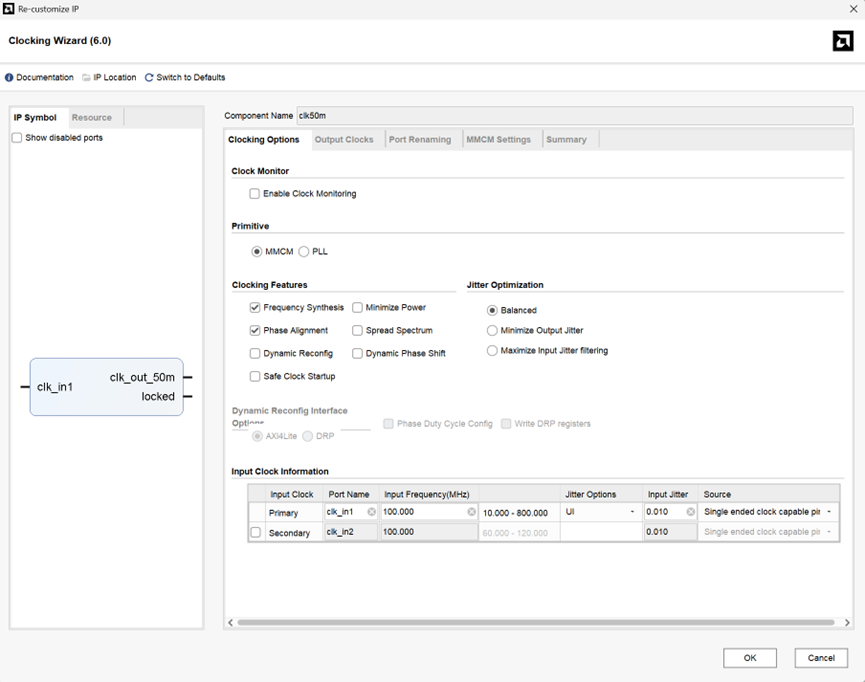
\includegraphics[width=0.45\textwidth]{figure/exp3/clk-1.png}}
  \hfill
  \subfloat[模块接口配置]{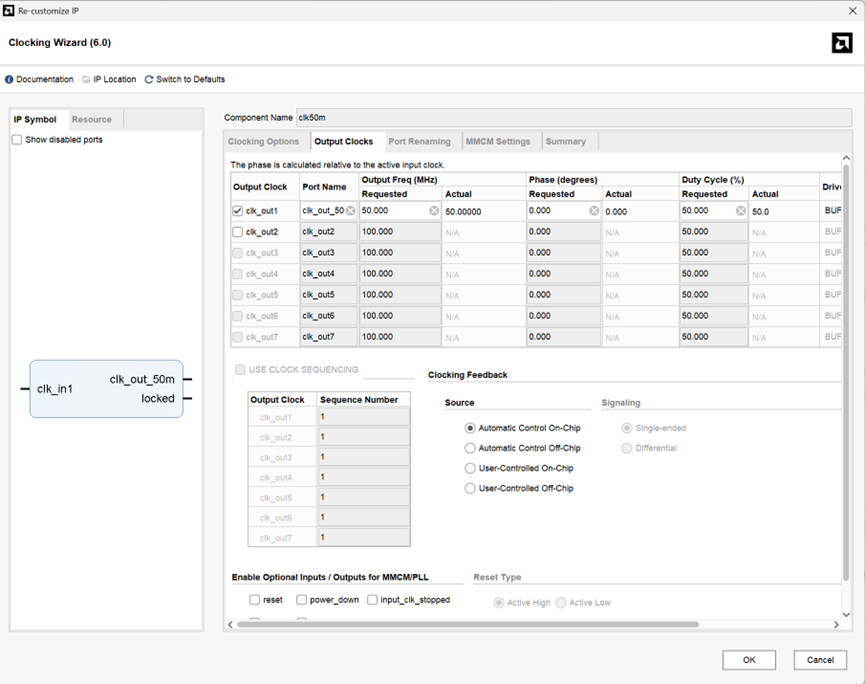
\includegraphics[width=0.45\textwidth]{figure/exp3/clk-2.png}}
  \caption{Clocking Wizard 配置信息}
  \label{fig:exp3:clk-1}
\end{figure}



\subsection{DDS Compiler IP Core配置1MHz和2MHz的余弦波}
在IP Catalog中搜索\textit{DDS Compiler} IP核。Vivado会自动弹出配置窗口。修改配置如图~\ref{fig:exp3:dds-1}~所示。由于同步时钟为50MHz,故DDS的时钟频率也需要和同步时钟频率相同;适当提高其无杂散动态范围 (SFDR, Spurious Frequency Dynamic Range)用来生成有用分量占比更大的余弦信号。配置结束后,将Output Frequency分别设置为1MHz和2MHz,例化两个模块。\footnote{实际的输出频率会略低于设定频率,这是由于DDS使用14-bit量化方案存储,会产生一定的量化误差。}
\begin{figure}[htbp]
  \centering
  \subfloat[模块配置]{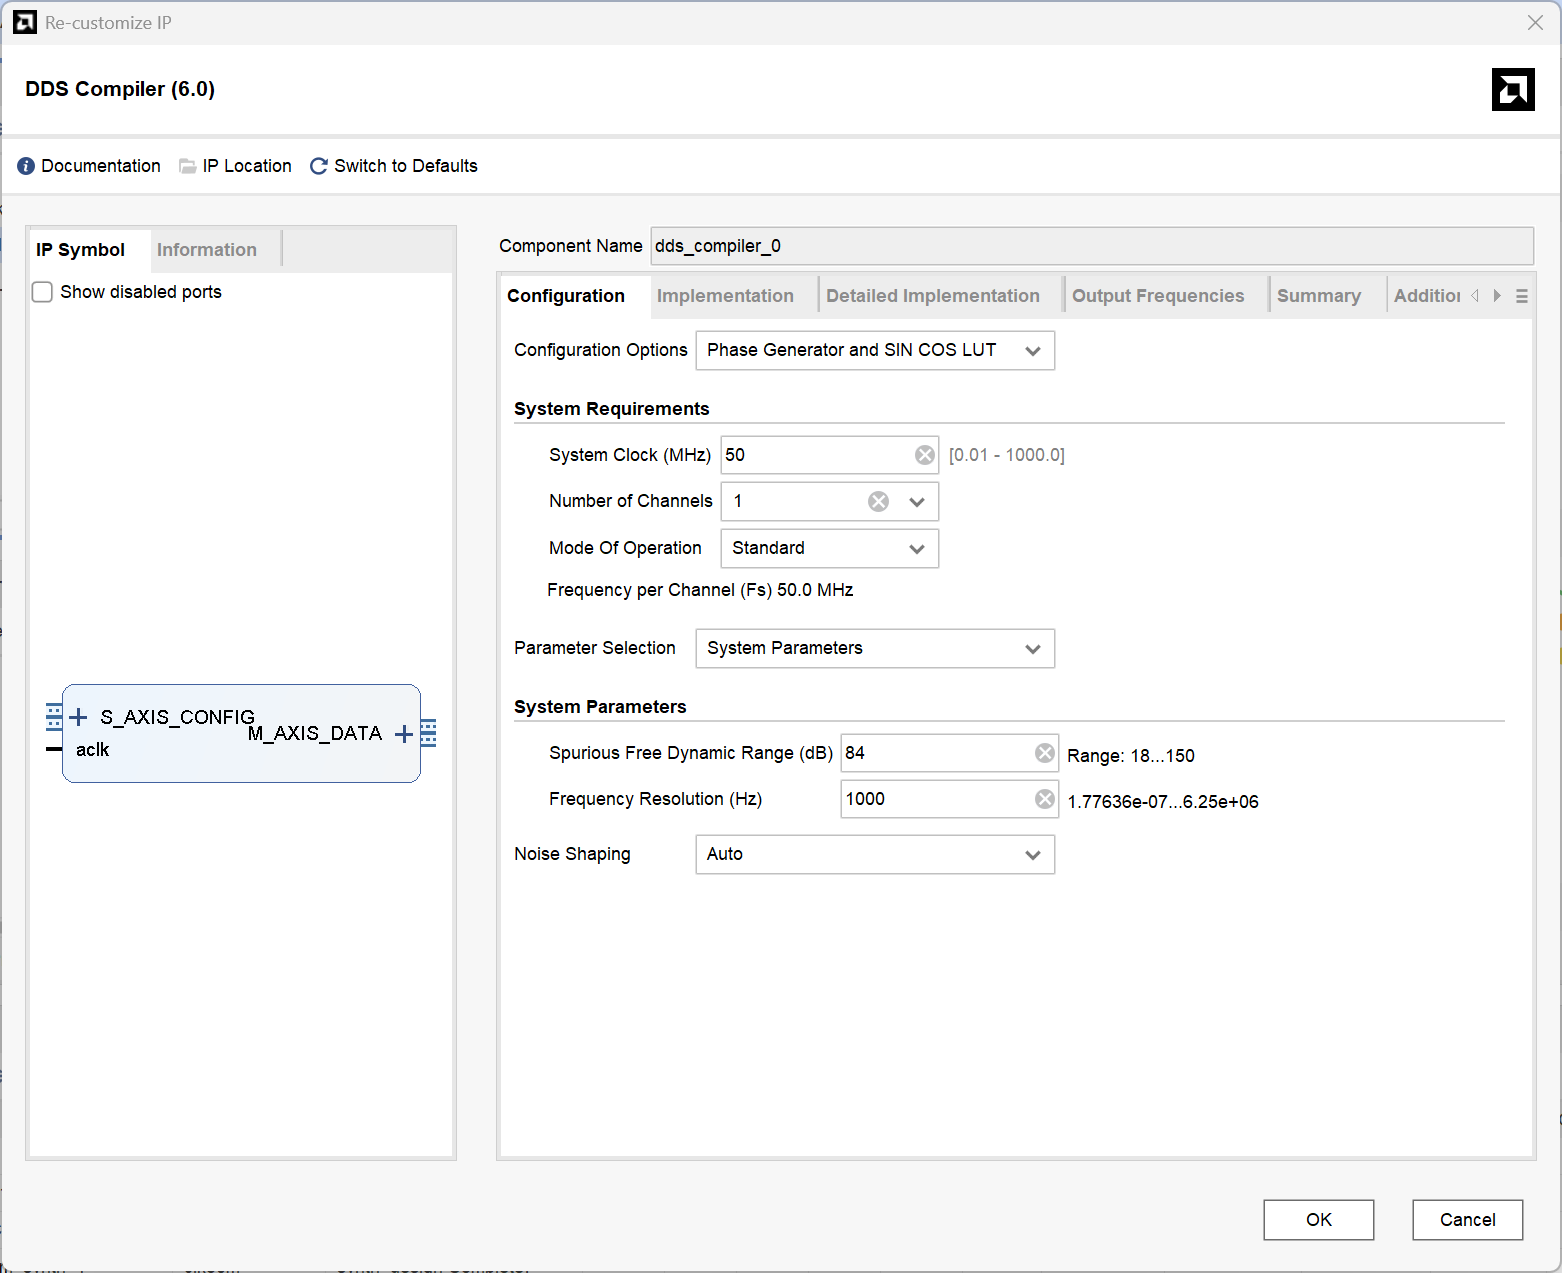
\includegraphics[width=0.45\linewidth]{figure/exp3/dds-1.png}}
  \hfill
  \subfloat[模块构建信息]{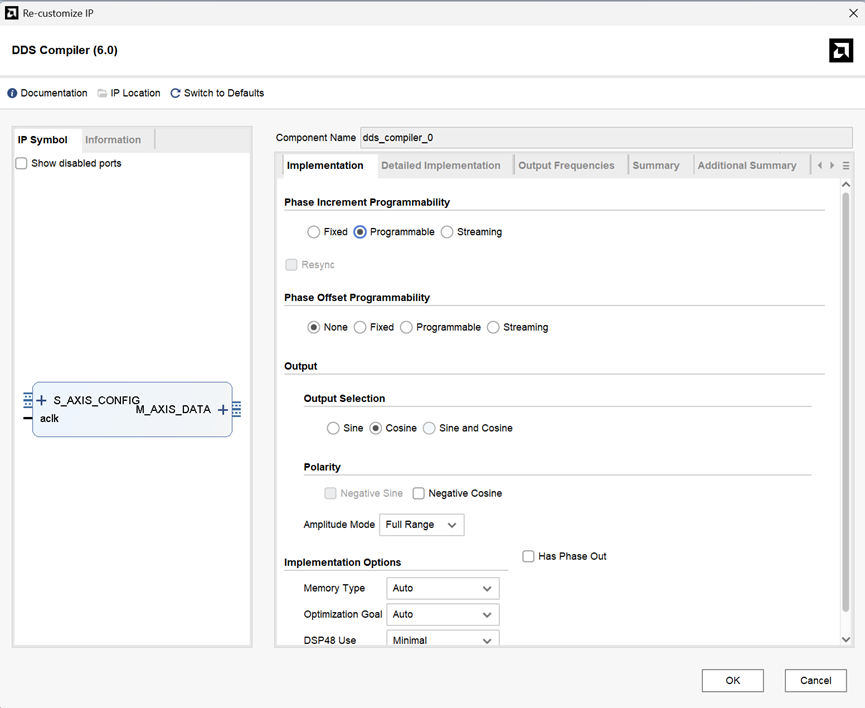
\includegraphics[width=0.45\linewidth]{figure/exp3/dds-2.png}}
  \caption{DDS Compiler配置信息}
  \label{fig:exp3:dds-1}
\end{figure}

\subsection{Integrated Logic Analyzer(ILA) IP Core配置}

Integrated Logic Analyzer(ILA)是 Xilinx 提供的一种片上调试工具,用于实时监测 FPGA 内部信号。ILA IP 核可以与 Vivado 逻辑分析仪(Logic Analyzer)协同工作,在不影响电路运行的情况下捕获关键信号,方便用户进行调试。

配置时,首先在 Vivado 的 \texttt{IP Catalog} 中搜索 \texttt{ILA},双击打开 IP 配置界面。在配置页面,用户设置以下参数:
\begin{itemize}
    \item \textbf{Probe 端口数量}:指定需要监测的信号数量,这里指定DAC之前的数字信号端口,\texttt{probe0}和\texttt{probe1}用来检测两种频率的余弦波。
    \item \textbf{每个 Probe 端口的数据宽度}:设置每个监测信号的位宽,通常与目标信号匹配。由于DAC的输出位宽为14-bit,此处位宽为14。
    \item \textbf{采样时钟}:ILA 需要连接 FPGA 内部的时钟信号,选择50MHz的系统时钟。
\end{itemize}

配置结束后,设置页面的参数如图~\ref{fig:exp3:ILA}~所示。
\begin{figure}[htbp]
  \centering
  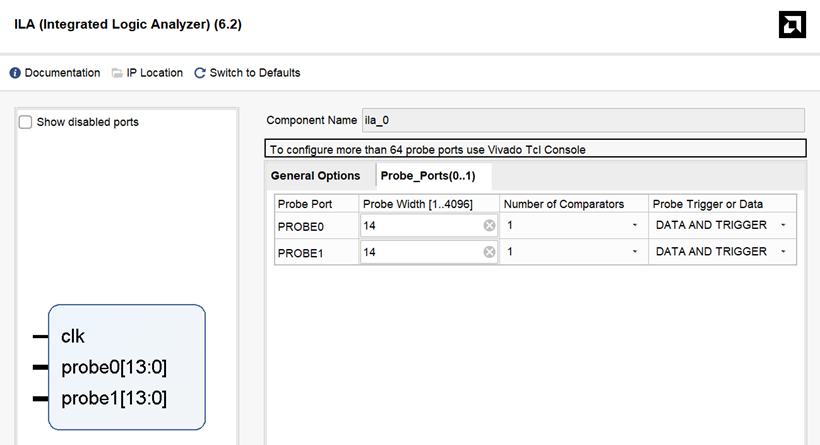
\includegraphics[width=0.75\textwidth]{figure/exp3/ila.png}
  \caption{ILA的IP核设置}
  \label{fig:exp3:ILA}
\end{figure}

在综合(Synthesis)和实现(Implementation)之后,用户需要生成比特流(Bitstream)。下载至 FPGA 后,打开 Vivado 的硬件管理器(Hardware Manager),连接开发板,加载比特流文件,就可以在右侧端口启动 ILA 仿真。


\subsection{利用IP核生成不同频率的余弦信号}
使用上述三个IP核的配置,编写Verilog代码:
\begin{lstlisting}[language=verilog]
`timescale 1ns / 1ps
module top_mod
(
	// DAC  PINS
  input PL_CLK_100MHz, 
  output signed [13:0] LS_DAC2_DB,   
	output LS_DAC2_CLK,              
	output LS_DAC2_WRT,         
	output signed [13:0] LS_DAC1_DB, 
  output LS_DAC1_CLK, 
	output LS_DAC1_WRT,
	output LS_DAC_MODE
);

	wire  clk_50M;                              // Storage of Clock
	wire clk_locked;                            // lock signal for clk
	wire signed [13:0] sin1M_data, sin2M_data;  // Storage of sine waves
	
	clk50m CLK_50M
    (
      // Clock out ports
      .clk_out_50m(clk_50M),     // output clk_out_50m
      // Status and control signals
      .locked(clk_locked),       // output locked
     // Clock in ports
      .clk_in1(PL_CLK_100MHz)      // input clk_in1
    );
    
  dds_compiler_0 DDS_1M_GENERATOR 
    (
      .aclk(clk_50M),                                  // input wire aclk
      .s_axis_config_tvalid(1'b1),  // input wire s_axis_config_tvalid
      .s_axis_config_tdata(16'H51E),    // input wire [15 : 0] s_axis_config_tdata
      .m_axis_data_tvalid(),      // output wire m_axis_data_tvalid
      .m_axis_data_tdata(sin1M_data)        // output wire [15 : 0] m_axis_data_tdata
    );
    
  dds_compiler_0 DDS_2M_GENERATOR 
    (  
      .aclk(clk_50M),                                  // input wire aclk
      .s_axis_config_tvalid(1'b1),  // input wire s_axis_config_tvalid
      .s_axis_config_tdata(16'HA3D),    // input wire [15 : 0] s_axis_config_tdata
      .m_axis_data_tvalid(),      // output wire m_axis_data_tvalid
      .m_axis_data_tdata(sin2M_data)        // output wire [15 : 0] m_axis_data_tdata
    );

   ila_0 ILA 
    (
	    .clk(clk_50M), // input wire clk
	    .probe0(sin1M_data), // input wire [13:0]  probe0  
	    .probe1(sin2M_data) // input wire [13:0]  probe1
    );
		
	// DAC OUTPUT
	assign LS_DAC_MODE = 1'b1;
	assign LS_DAC1_DB = sin1M_data + 14'h2000;
	assign LS_DAC1_CLK = !clk_50M;
	assign LS_DAC1_WRT = LS_DAC1_CLK;
	assign LS_DAC2_DB = sin2M_data + 14'h2000;
	assign LS_DAC2_CLK = clk_50M;
	assign LS_DAC2_WRT = LS_DAC2_CLK;

	
endmodule
\end{lstlisting}

进入Vivado界面,确认IP核与约束文件设置正确后,点击“生成Bitstream”将完成综合、构建和比特流生成。\footnote{需要确认例化的模块中的变量名和IP核中设置的完全相同,否则Vivado无法综合。}

将电脑与 eNodeX 软件无线电创新平台相连接,该平台内置有一块FPGA(xc7z020clg484-1)用于烧录本机程序,并给出两个通道的输出接口,用于连接示波器的两个通道。之后选择“Auto Detect Target”选择连接好的设备,按下“Program Device”将程序烧录到FPGA中。若示波器正常连接,可以看到两个通道显示了1MHz和2MHz的余弦波(图~\ref{fig:exp3:waveform}~)。\footnote{需要按下\texttt{RUN/STOP}才能正常显示波形。}

\begin{figure}[htbp]
  \centering
  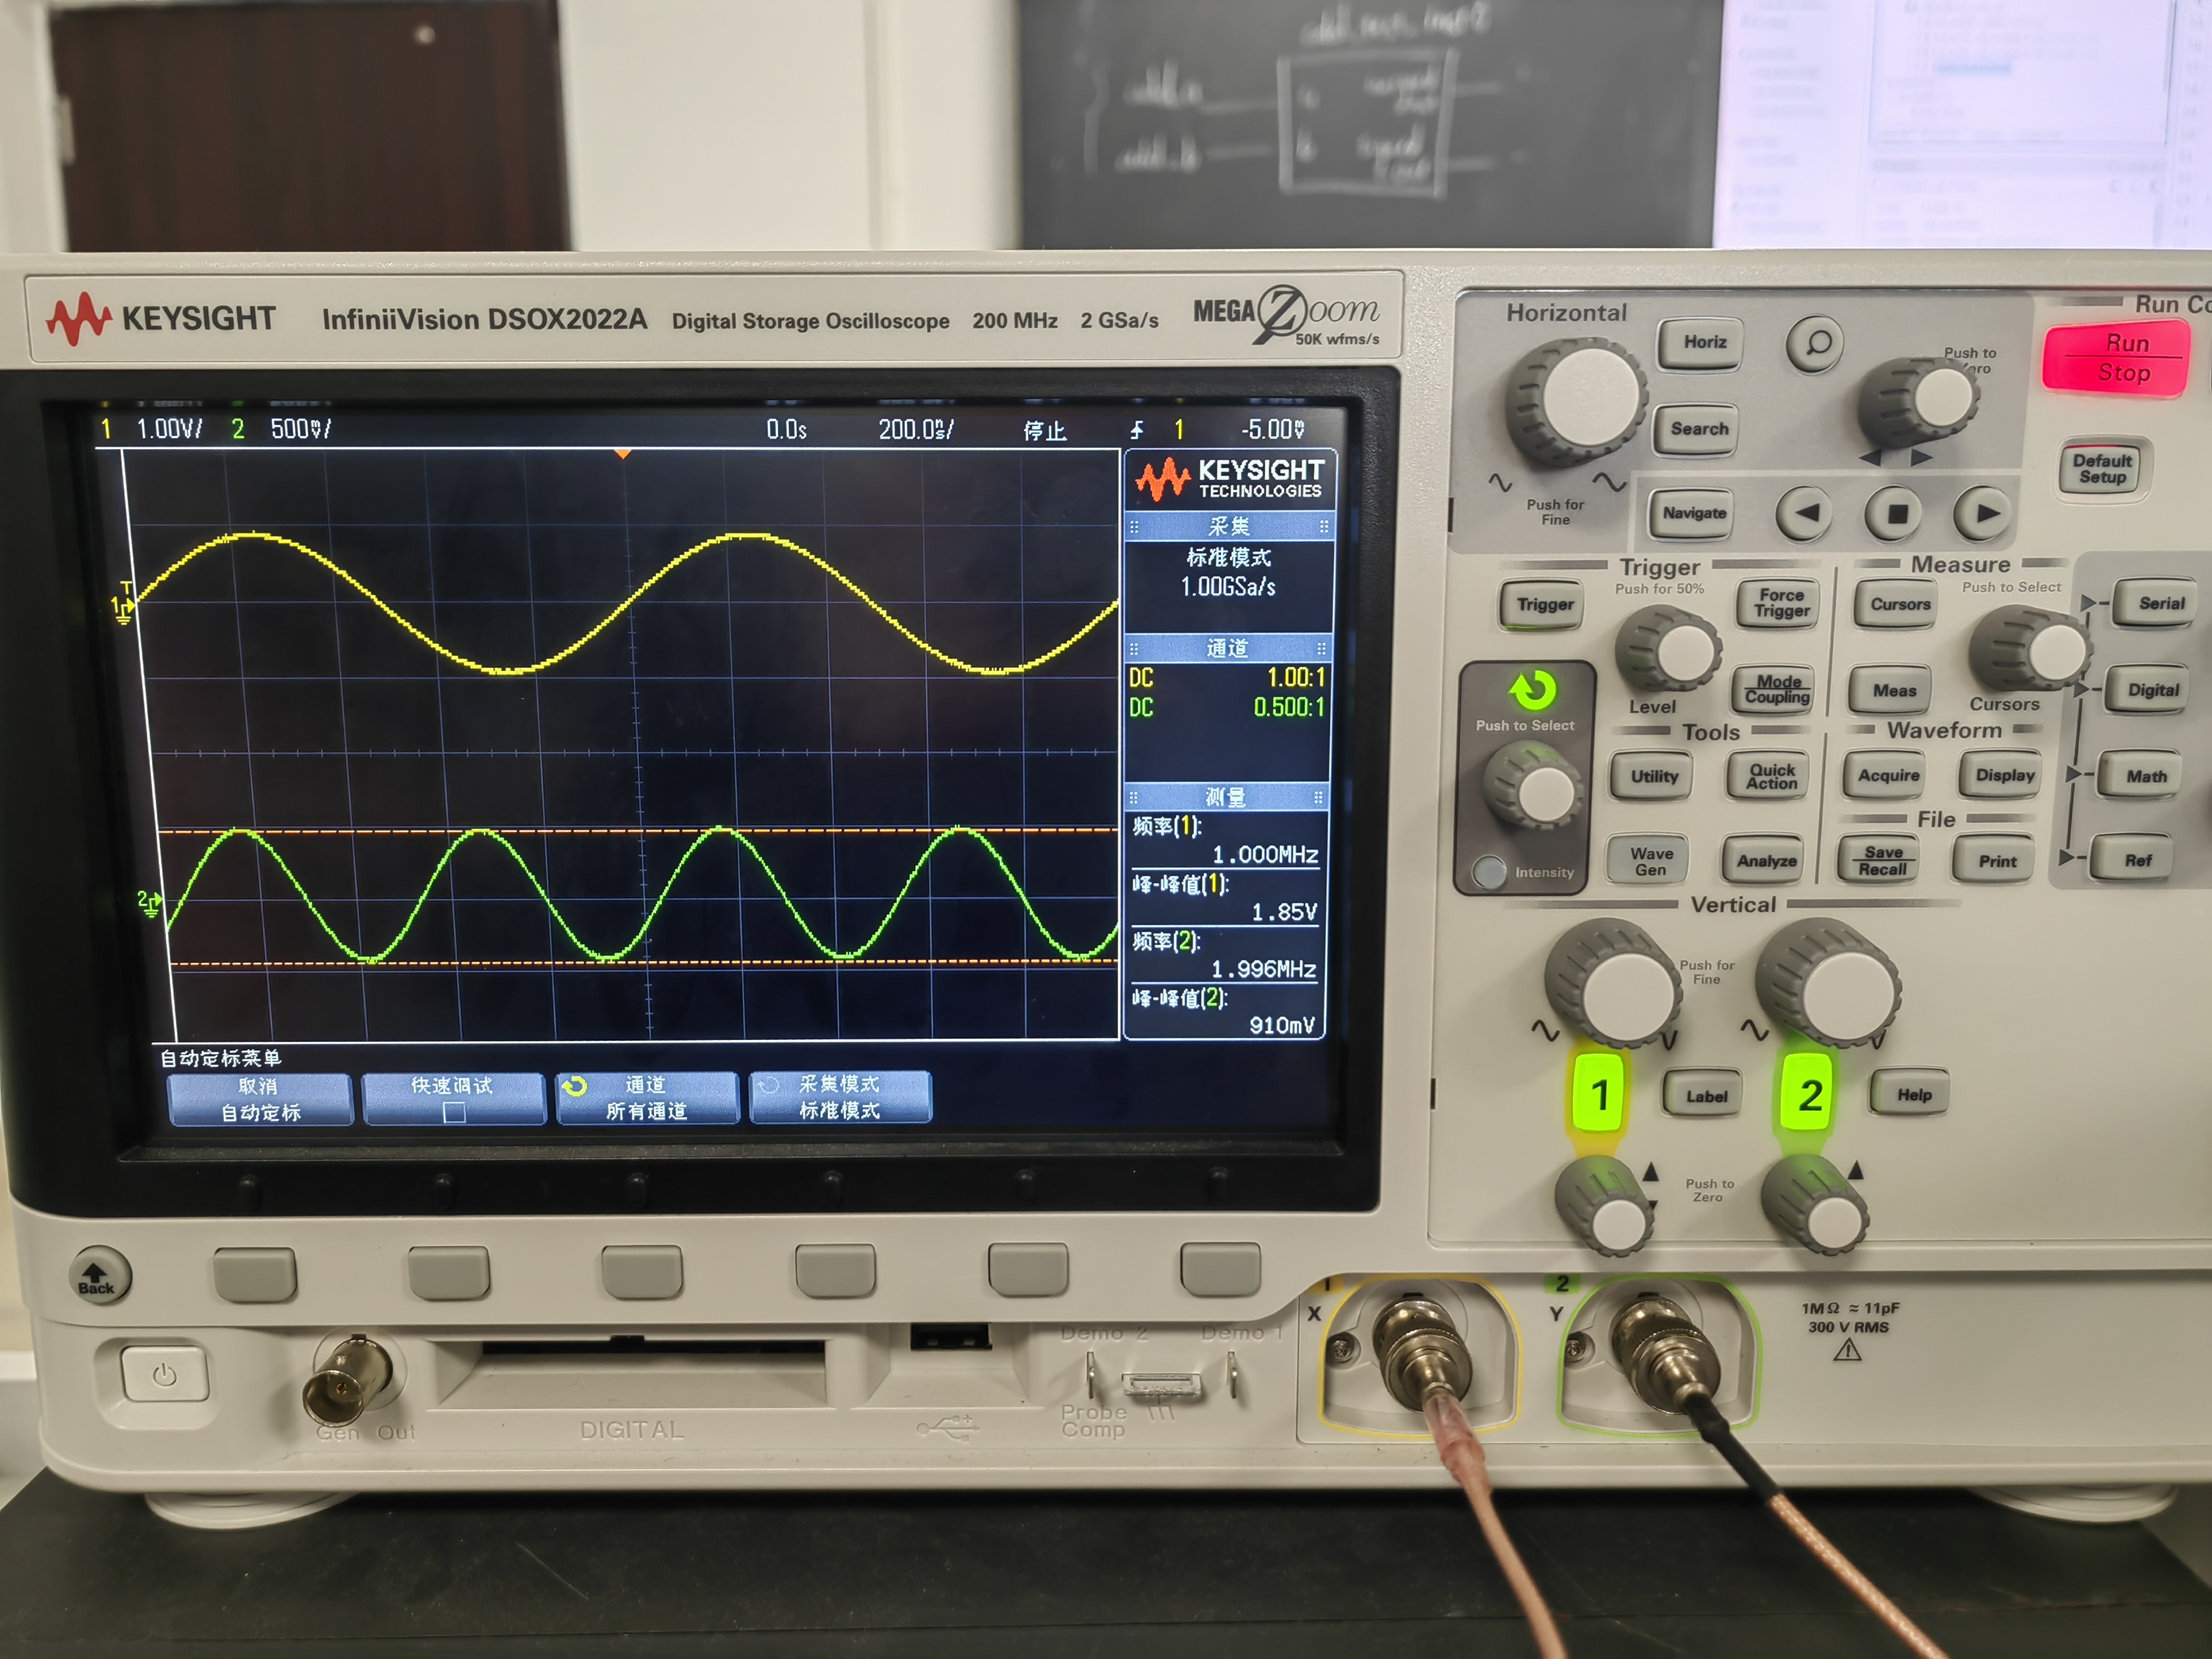
\includegraphics[width=0.75\textwidth]{figure/exp3/waveform.jpg}
  \caption{示波器波形}
  \label{fig:exp3:waveform}
\end{figure}

另外,在写入Bitstream之后,启动xsim,可以观察到ILA检测的两个余弦波的14-bit量化数据(即DAC之前的采样数据)如图~\ref{fig:exp3:sim}~。
\begin{figure}[htbp]
  \centering
  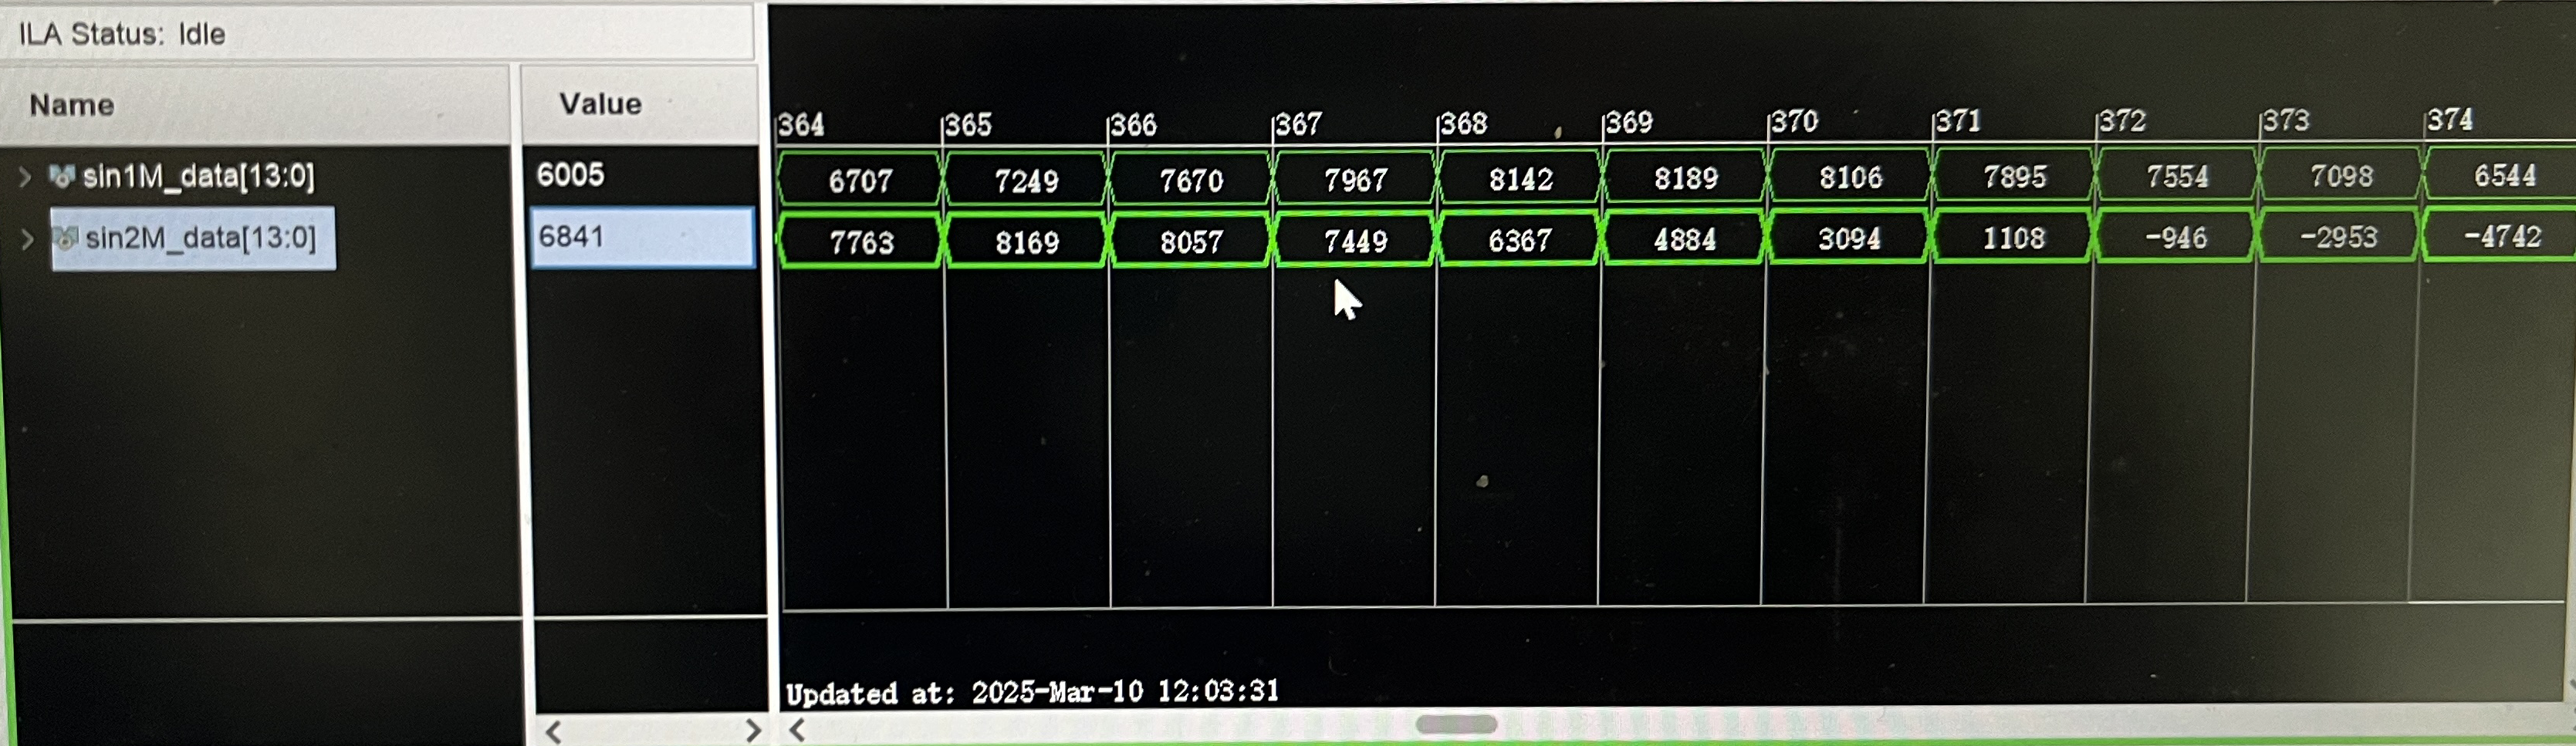
\includegraphics[width=0.75\textwidth]{figure/exp3/sim.png}
  \caption{余弦波的采样数据}
  \label{fig:exp3:sim}
\end{figure}


% \chapter{基于累加器的FIR滤波器设计}
\begin{introduction}
  \item \textit{使用Simulink进行FIR滤波器的仿真;}
  \item \textit{MATLAB绘制FIR滤波器的输入输出响应;}
  \item \textit{Verilog编写简单的FIR滤波器;}
  \item \textit{基于累加器的FIR滤波器的FPGA实现。}
\end{introduction}
\section{实验背景与目的}
随着 FPGA(Field Programmable Gate Array)技术的广泛应用,数字信号处理(DSP)在通信、音频处理和工业控制等领域的需求不断增长。FIR(有限脉冲响应)滤波器作为一种重要的数字滤波技术,以其线性相位特性和稳定性,在硬件实现中占据重要地位。

在 FPGA 设计中,乘法-累加(MAC)运算是 FIR 滤波器的核心计算过程,而累加器结构能够高效执行这一运算,提高计算吞吐量和资源利用率。本实验围绕 FIR 滤波器的硬件实现,重点研究基于累加器的FIR滤波器实现方法,并结合 MATLAB 和 Simulink 进行算法仿真,以验证滤波器性能。另外,通过本实验,还可以进一步熟悉Vivado IP核的调用方法。

\section{实验原理}

\subsection{FIR 滤波器}

有限脉冲响应(Finite Impulse Response, FIR)滤波器是一种线性时不变系统,其输出仅依赖于当前及有限个历史输入样本,而不会受到过去输出的影响。其数学表达式为:

\begin{equation}
    y[n] = \sum_{k=0}^{N-1} h[k] x[n-k]
\end{equation}

其中:
\begin{itemize}
    \item $x[n]$ 为输入信号,
    \item $y[n]$ 为输出信号,
    \item $h[k]$ 为滤波器系数(即脉冲响应),
    \item $N$ 为滤波器的阶数。
\end{itemize}

FIR 滤波器的一个重要特点是其\textbf{线性相位特性},即滤波器系数满足对称性:

\begin{equation}
    h[k] = \pm h[N-1-k], \quad k = 0,1,\dots, N-1
\end{equation}

这种特性保证了不同频率分量不会产生相位失真,在许多信号处理应用中至关重要。

\subsection{FIR 滤波器的结构}

FIR 滤波器的实现主要基于乘积求和,可以采用直接型(横截型)、线性相位型和频率采样型等结构。最容易实现的是直接型结构。


直接型 FIR 滤波器的基本组成部分包括:
\begin{itemize}
    \item 延迟单元(Delay Elements):用于存储输入数据 $x[n]$ 的历史值,通常使用移位寄存器实现。
    \item 乘法器(Multipliers):将输入信号的延迟版本与滤波器系数 $h[k]$ 相乘。
    \item 加法器(Adders):对所有乘积求和,生成最终的滤波器输出。
\end{itemize}

在 FPGA 设计中,FIR 滤波器可以通过 乘法-累加(MAC, Multiply-Accumulate) 结构优化计算效率,同时利用 DSP 资源 进行并行计算,提高吞吐量。此外,为了减少乘法运算,通常采用系数量化和移位累加(Shift-and-Add)技术。

本实验将基于 FPGA 设计一个 FIR 滤波器,并采用累加器结构进行优化,以提高计算性能和资源利用率。
\section{实验使用软件/平台}
\begin{itemize}
  \item Xilinx Vivado 2024.2;\footnote{笔者在这次实验时将Vivado部署到了Linux中,Implementation的速度远高于Windows,且官网可以下载到免费的版本。配置的过程见本章结尾。}
  \item eNodeX 30B软件无线电创新平台;
  \item 示波器。
  \item MATLAB \& Simulink R2024b;
\end{itemize}
\section{实验内容}
\subsection{FIR滤波器的Simulink仿真}
为了直观描述FIR数字滤波器的结构,使用Simulink搭建两种结构的FIR数字滤波器。其中第二种并不常见,且实现起来无法复用延时器,故仅作仿真用。

\begin{figure}[htbp]
  \subfloat[横截型FIR滤波器\label{subfig:hengjie}]{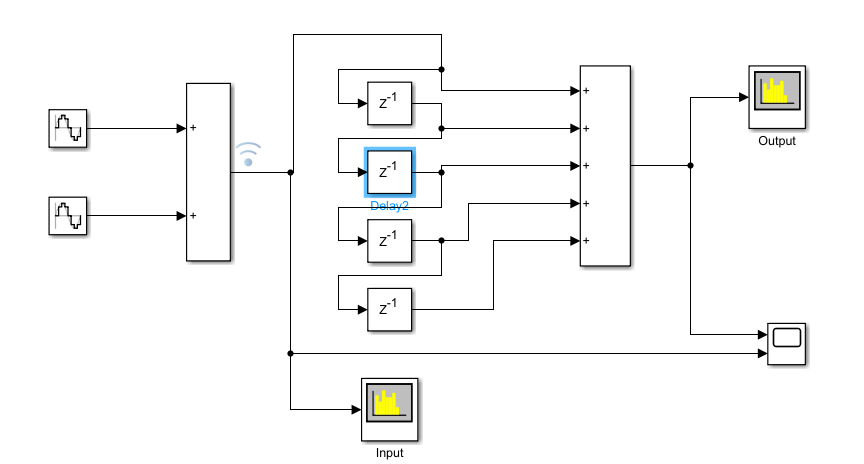
\includegraphics[width = 0.45\textwidth]{figure/exp4/circuit_exp4.png}}
  \hfill
  \subfloat[FIR滤波器]{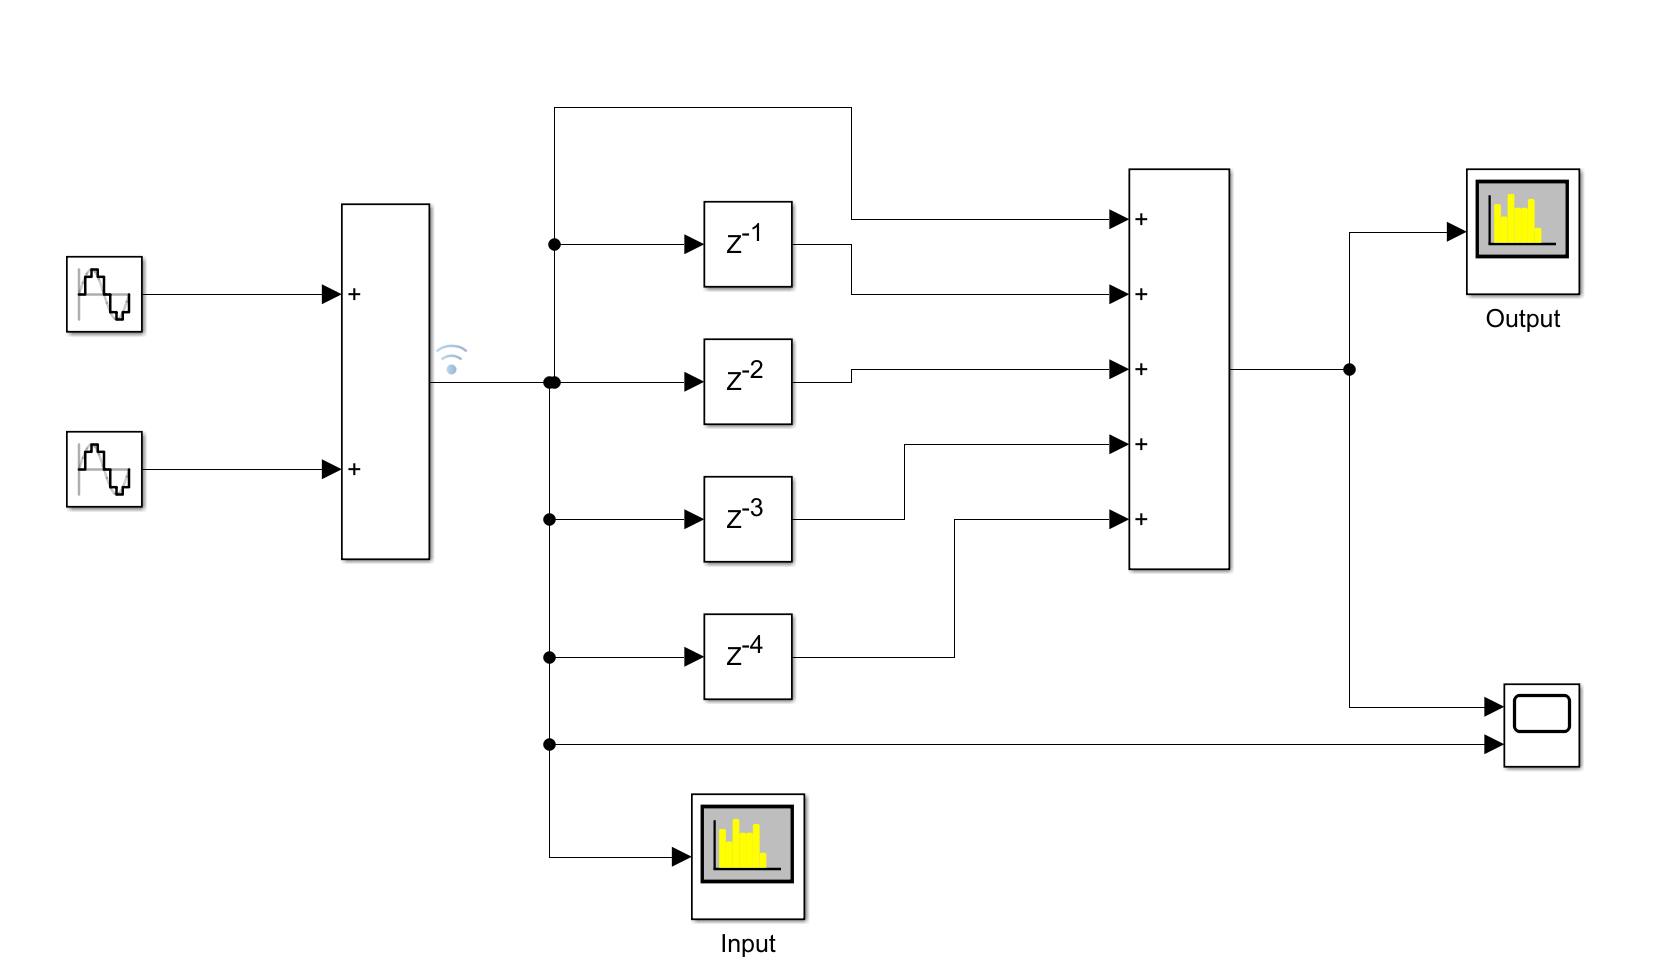
\includegraphics[width = 0.45\textwidth]{figure/exp4/circuit_exp4_2.png}}
  \caption{两种FIR滤波器的结构}
  \label{fig:exp4:simulink}
\end{figure}
搭建两种结构的数字滤波器如图~\ref{fig:exp4:simulink}。图~\ref{subfig:hengjie}~是典型的横截型滤波器结构,输入为1MHz和10MHz的两股正弦信号经过加法器后通过该滤波器输出。滤波器由四个延时器和一个加法器组成,这在模型中也直观地体现出来了。第二种结构采用了四种不同的延时器,分别延时1、2、3、4个单位时钟,这让我们清楚地推出FIR滤波器的系统函数:
\begin{equation}\label{eqn:fir}
  H(z) = 1 + z^{-1} + z^{-2} +z^{-3} +z^{-4}
\end{equation}
令$z = e^{j\omega}$,可得系统的频率响应,显然可以看出该滤波器是一个低通滤波器。

启动仿真,观察滤波前和滤波后的时域波形如图~\ref{fig:exp4:scope}。可以看到,滤波前信号含有大量高频杂波,而滤波后信号变平滑。滤波后信号有约5倍的增益,这可以从公式~\ref{eqn:fir}~中找到原因。

\begin{figure}[htbp]
  \centering
  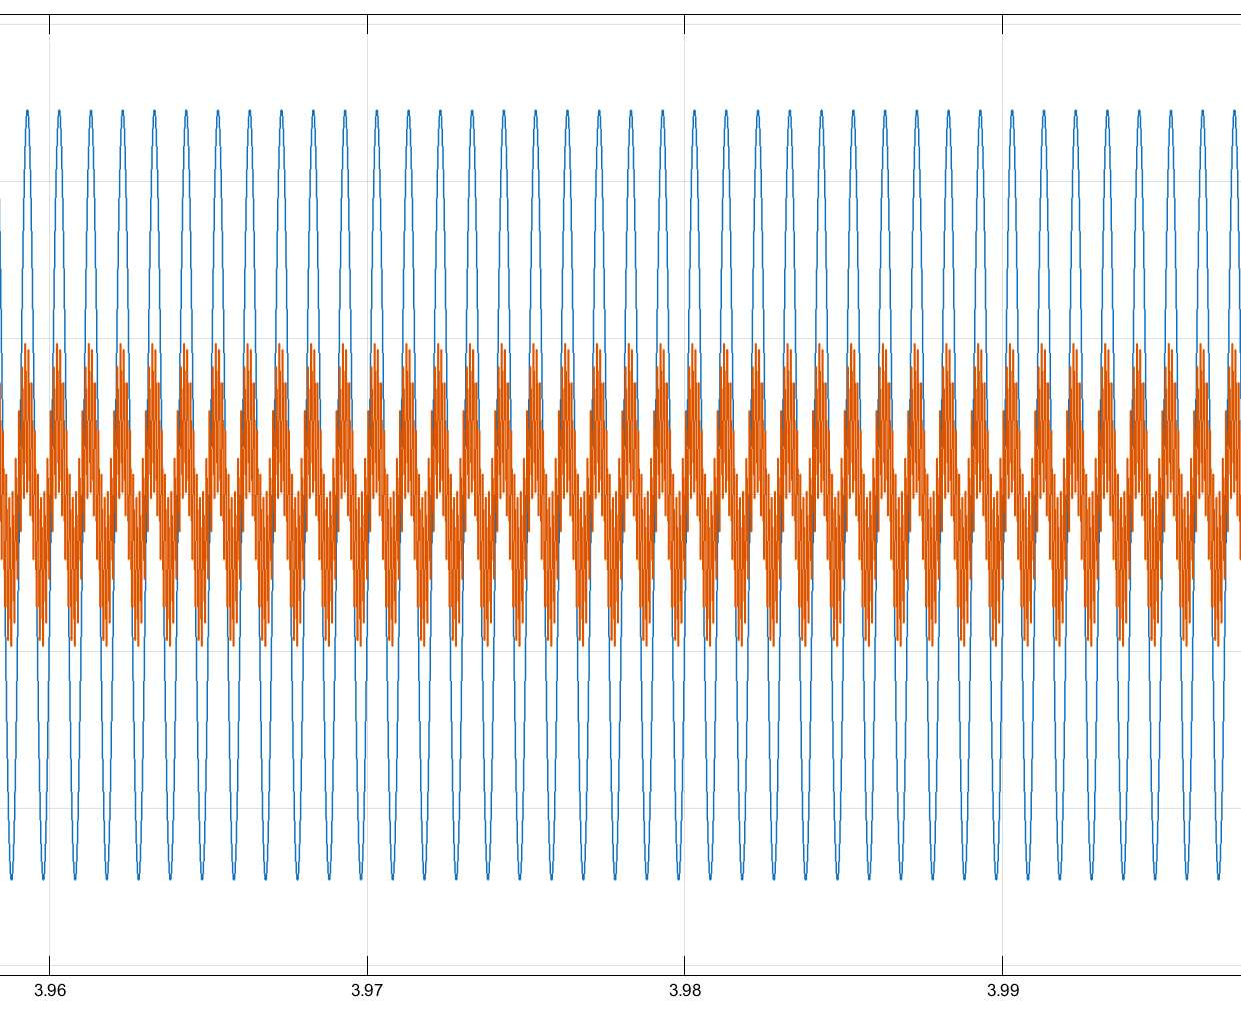
\includegraphics[width = 0.75\textwidth]{figure/exp4/scope.pdf}
  \caption{滤波前(橙)和滤波后(蓝)的时域波形}
  \label{fig:exp4:scope}  
\end{figure}

接下来进行频谱分析(图~\ref{fig:exp4:spectrum}~)。可以看出滤波前信号在1M和10M处包含峰值,这符合加和信号的特征;滤波后,高频分量被滤除,而低频分量出现一定失真。

\begin{figure}[htbp]
  \centering
  \subfloat[滤波前信号频谱]{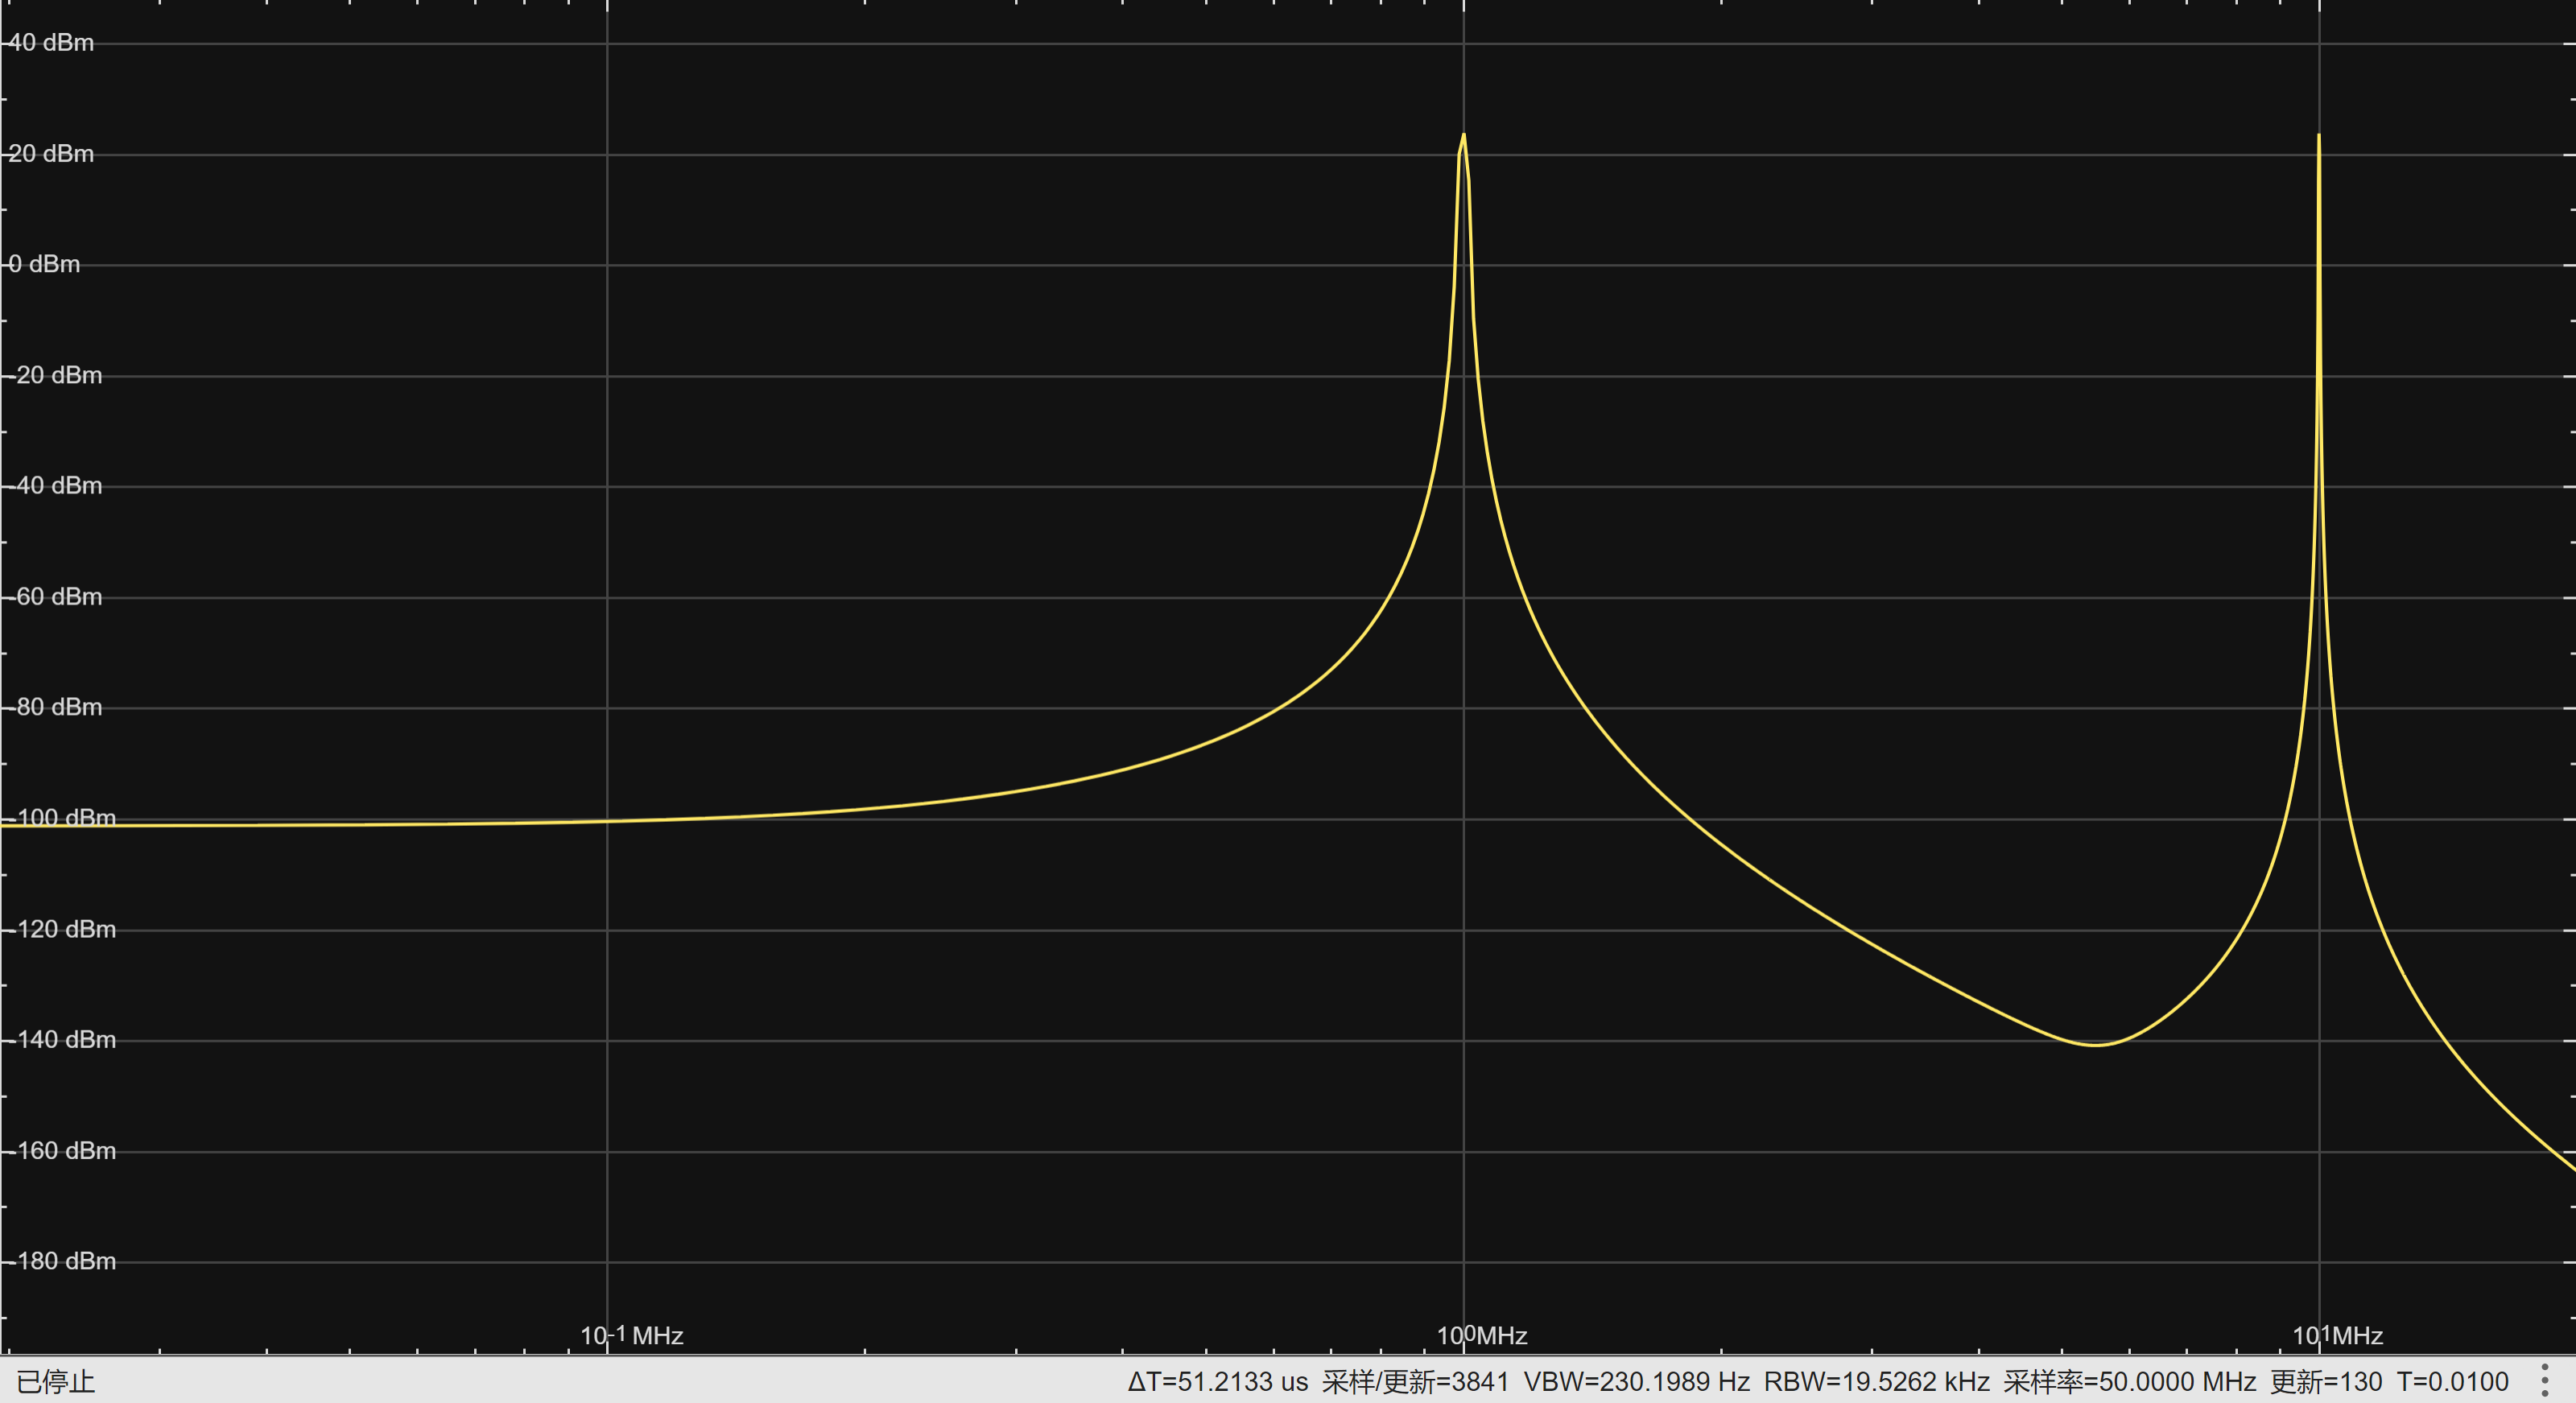
\includegraphics[width = 0.45\textwidth]{figure/exp4/input.png}}
  \hfill
  \subfloat[滤波后信号频谱]{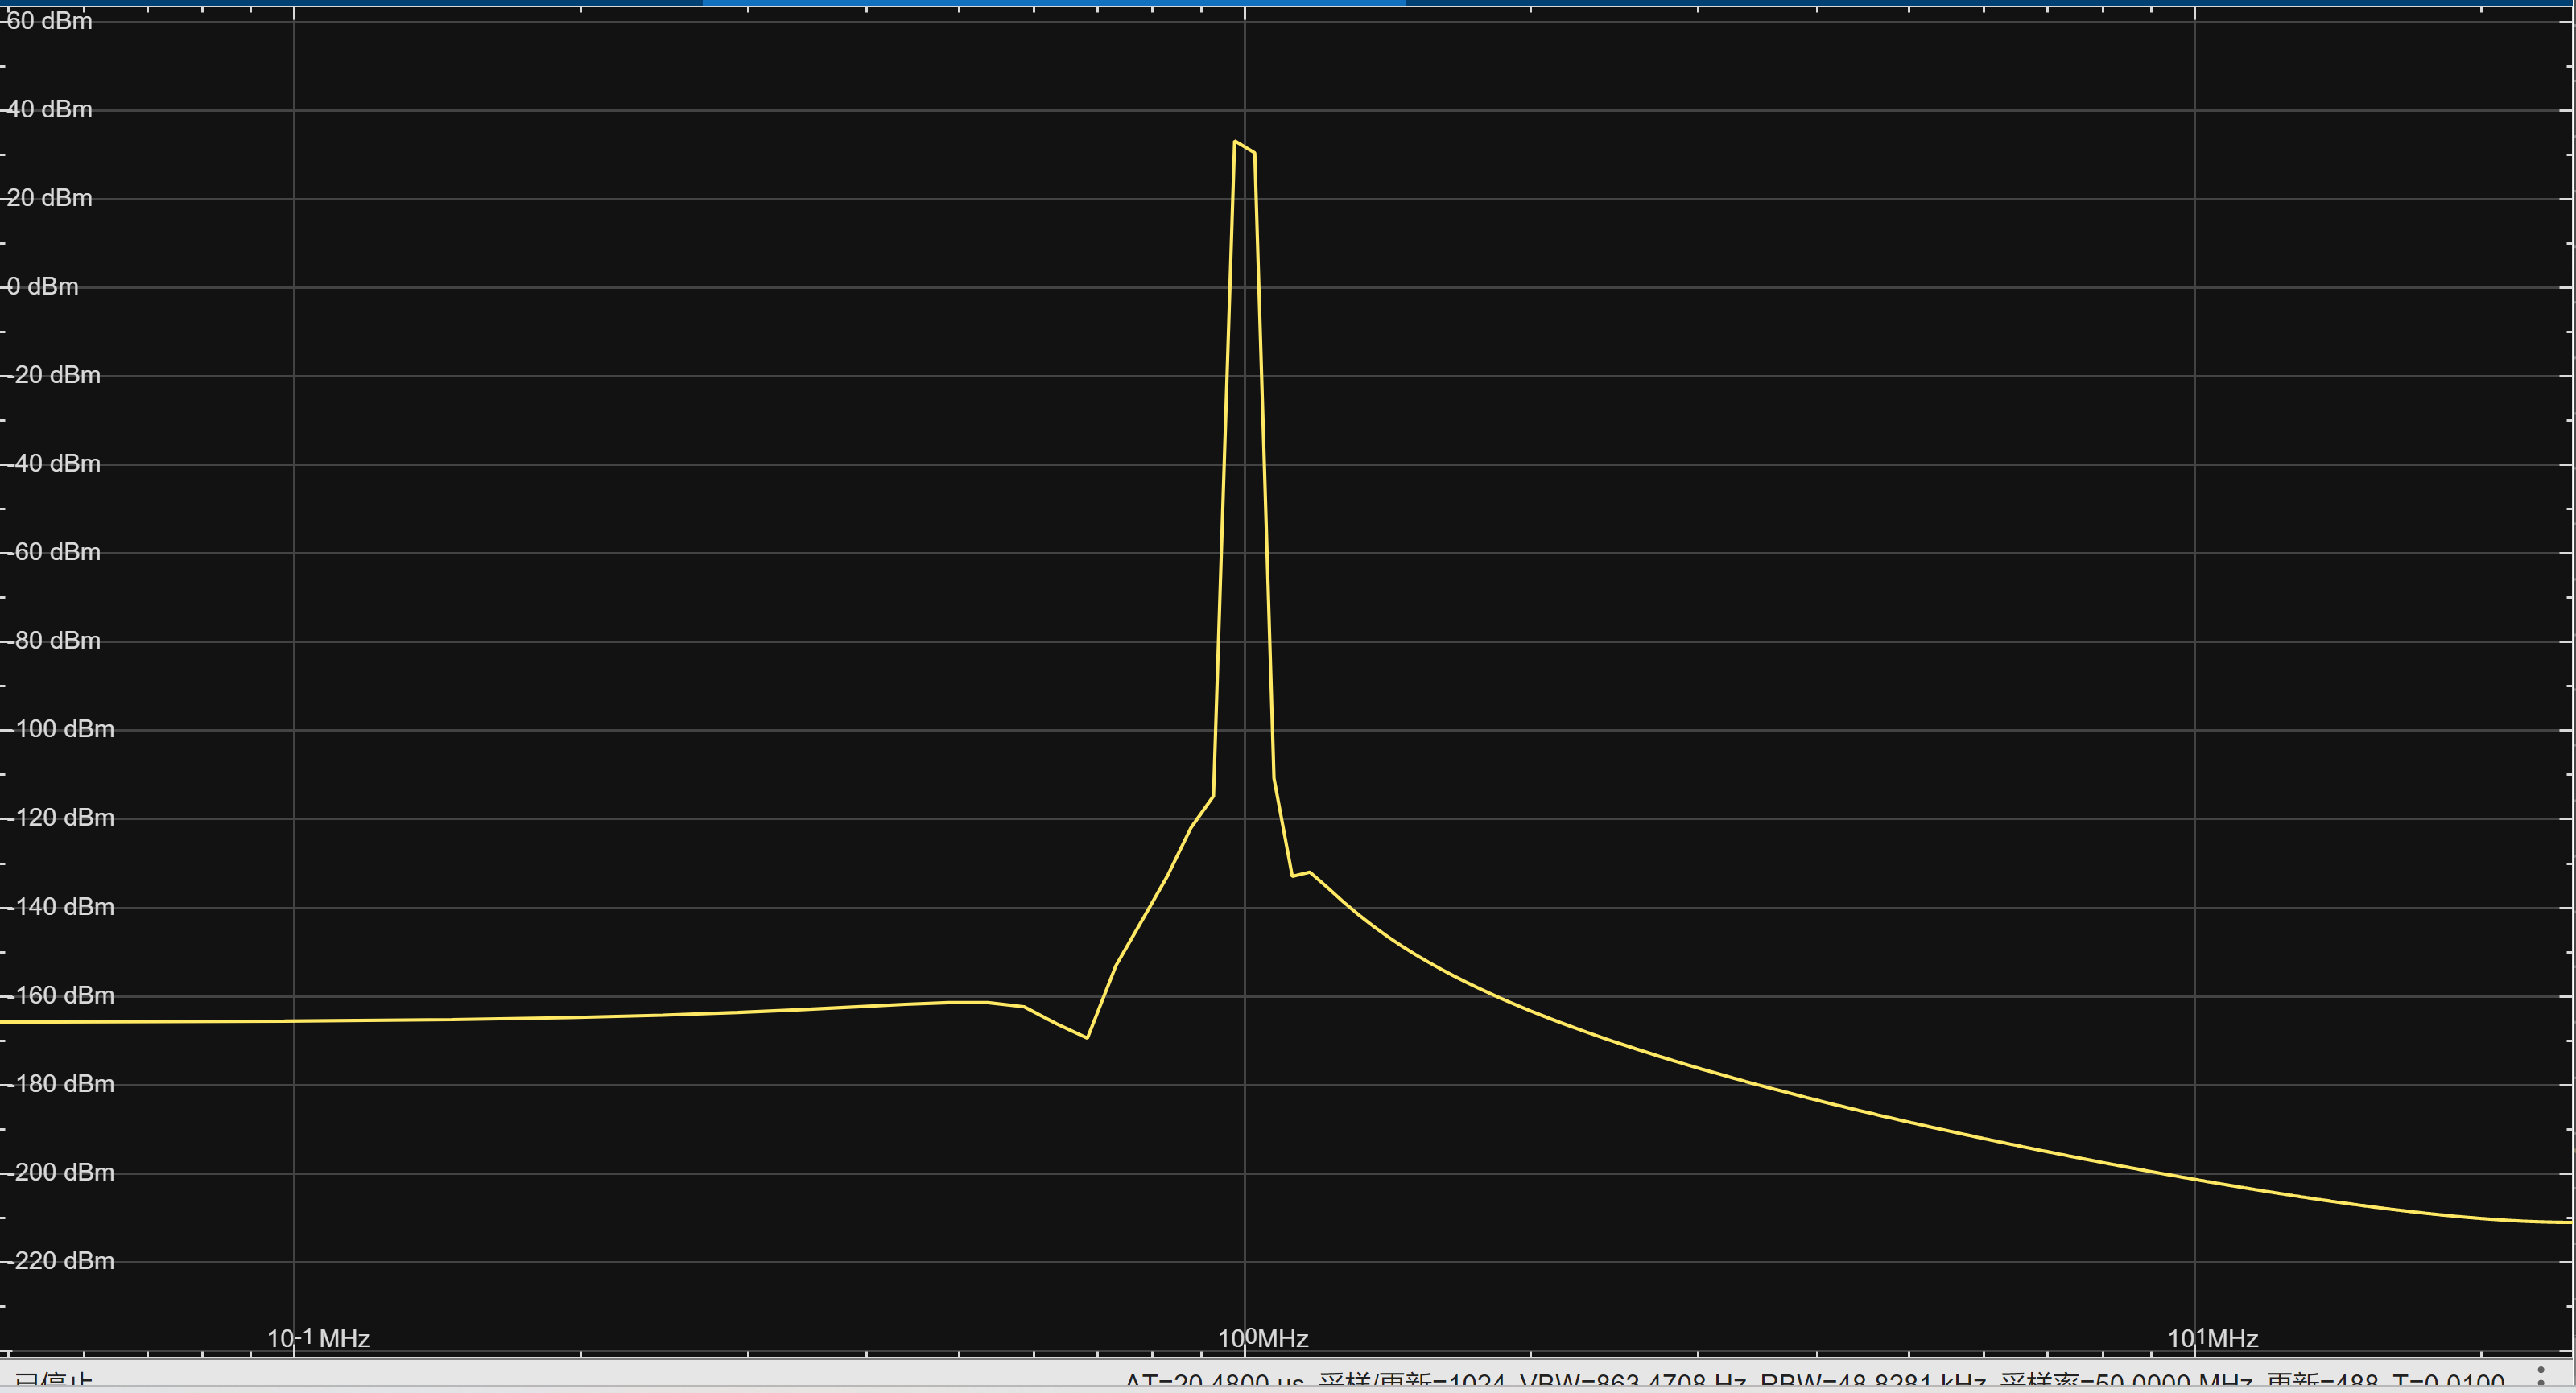
\includegraphics[width = 0.45\textwidth]{figure/exp4/output.png}}
  \caption{信号频谱分析}
  \label{fig:exp4:spectrum}
\end{figure}

\begin{remark}
两种形式的滤波器仿真结果相同,此处不再展示第二种滤波器的仿真结果。
\end{remark}

\subsection{FIR滤波器的MATLAB仿真}
编写MATLAB代码如下:
\begin{lstlisting}[language=matlab]
f1=1e7;
f2=1e6;
fs=5e7;
t=0:1/fs:0.00005;

s=sin(2*pi*f1*t)+sin(2*pi*f2*t); %产生两个频率信号的叠加信号
b=[1,1,1,1,1];
y=filter(b,1,s);
%累加器(滤波器)的系数
%求出滤波器输出序列

%第1张图绘制输入输出信号
figure(1);
subplot(211); plot(t,s);
legend('输入信号波形');
xlabel('时间(s)');ylabel('幅度(v)');
subplot(212);plot(t,y);
legend('输出信号波形');
xlabel('时间(s)');ylabel('幅度(v)');
%第2张图绘制滤波器频率响应
figure(2);
freqz(b,1)
\end{lstlisting}
运行代码,可得到输入输出信号的波形,以及滤波器的频率响应如图~\ref{fig:exp4:matlab}。
\begin{figure}[htbp]
  \centering
  \subfloat[滤波前后信号波形]{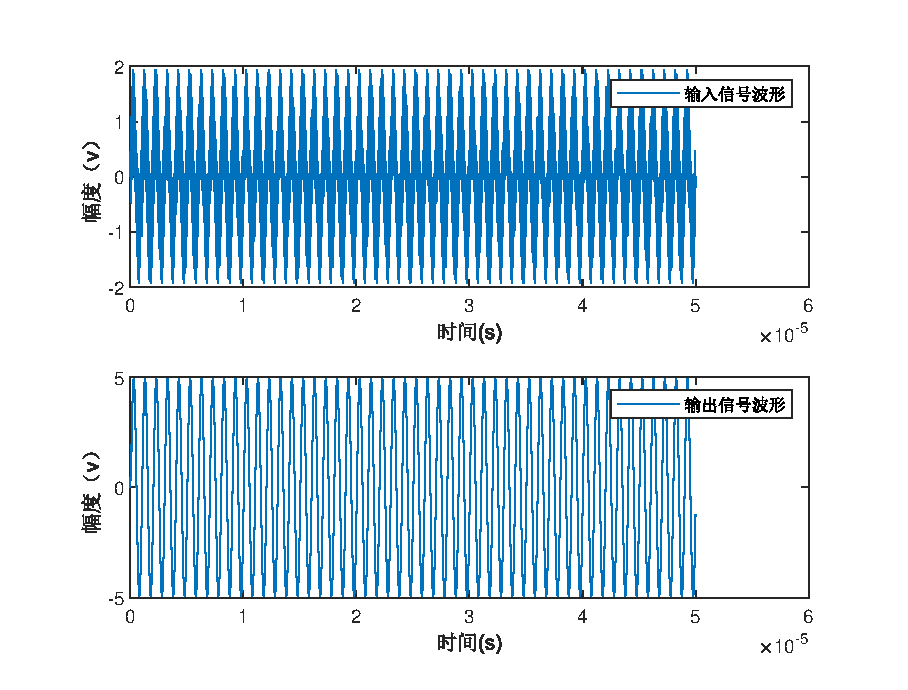
\includegraphics[width = 0.45\textwidth]{figure/exp4/fig1.eps}}
  \hfill
  \subfloat[滤波器的频率响应]{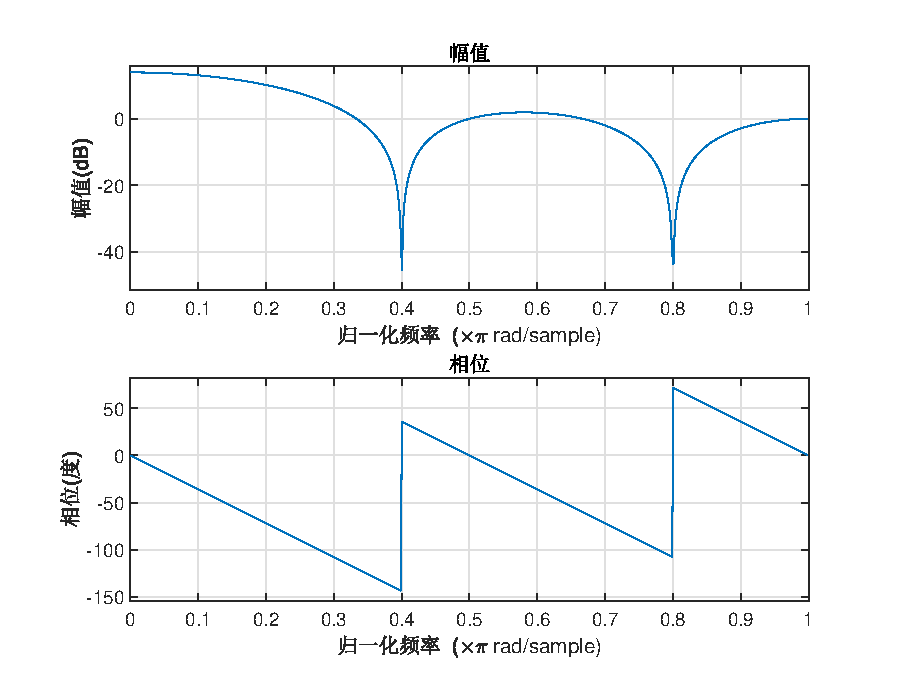
\includegraphics[width = 0.45\textwidth]{figure/exp4/fig2.eps}}
  \caption{信号频谱分析}
  \label{fig:exp4:matlab}
\end{figure}
\subsection{基于累加器的FIR滤波器的FPGA实现}
基于公式~\ref{eqn:fir}~和图~\ref{subfig:hengjie},可以设计一个基于累加器的FIR滤波器。需要注意的是,由于输出为五个输入相加,故输出的最大可能位宽为输入位宽+4。FIR滤波器的输入输出端口如表~\ref{table:interface_fir}~所示。

\begin{table}[htbp]
  \centering
  \begin{tabular}{ccc}
    \toprule
     信号名 & 意义 & 端口类型\\
    \midrule
      \texttt{clk} & 50MHz时钟信号 & Input \\
     \texttt{xin} & 10-bit 加和后量化正弦信号 & Input \\
     \texttt{yout} & 14-bit 滤波后量化信号输出 & Output \\
    \bottomrule
  \end{tabular}
  \caption{FIR模块接口说明}
  \label{table:interface_fir}
\end{table}

下面是该模块的代码,可见输入数据通过4个寄存器后生成四个时刻的数据,再相加得到滤波器的输出。
\begin{lstlisting}[language=verilog,caption={FIR滤波器模块}]
module FIR(
      input clk,                      // 50MHz Clock
      input signed [10:0] xin,        // input
      output signed [13:0] yout       // output
  );
  
  reg signed [10:0] x1,x2,x3,x4; // cascaded registers
  always @(posedge clk) begin
  x1 <= xin; 
  x2 <= x1; 
  x3 <= x2; 
  x4 <= x3;
  end
  
  // Output
  assign yout =xin + x1 + x2 + x3 + x4; 
  endmodule
  \end{lstlisting}
\begin{lstlisting}[language=verilog, caption={Testbench文件}]
  `timescale 1ns / 1ps

  module tb_FIR;
  
  reg clk;    // 100MHz
  reg clk_DAC1, clk_DAC2, wrt_DAC1, wrt_DAC2;
  reg mode_DAC;
  reg [13:0] filter_input;
  reg [13:0] filter_output;
  
  
  TOP module_top(
  .PL_CLK_100MHz(clk), 
  .LS_DAC2_DB(filter_output),
  .LS_DAC2_CLK(clk_DAC2),
  .LS_DAC2_WRT(wrt_DAC2),
  .LS_DAC1_DB(filter_input),
  .LS_DAC1_CLK(clk_DAC1),
  .LS_DAC1_WRT(wrt_DAC1),
  .LS_DAC_MODE(mode_DAC)
  );
  
  //clock
  initial begin
  clk = 0; 
  end 
  always #5 clk <= !clk;    
  
  initial begin
      $dumpfile("fir.vcd");
      $dumpvars(0, tb_FIR);
  end
  
  initial begin
  #1000000 $stop(2);
  end
  
  endmodule
  
\end{lstlisting}

基于此模块设计,编写测试模块(Testbench)如下。在测试模块中调用\textit{DDS Compiler} IP核生成1MHz和10MHz的正弦信号并相加后,对FIR模块进行测试。
\begin{lstlisting}[language=verilog, caption={Testbench文件}]
  `timescale 1ns / 1ps
  module tb_FIR;
  
    reg clk;
    wire signed [10:0] xin;  // FIR Input
    wire signed [13:0] yout;  // FIR Output
    wire signed [9:0] sin1M, sin10M;  // Generated by DDS
  
  
    FIR DUT (
        .clk (clk),
        .xin (xin),
        .yout(yout)
    );
  
    // Generate 50MHz Clock signal for testbench
    initial begin
      clk = 0;
    end
  
    always #10 clk <= ~clk;
    
    SIN_1M sin_1M (
        .aclk                (clk),      // input wire aclk
        .s_axis_config_tvalid(1'b1),     // input wire s_axis_config_tvalid
        .s_axis_config_tdata (16'H51E),  // input wire [15 : 0] s_axis_config_tdata
        .m_axis_data_tvalid  (),         // output wire m_axis_data_tvalid
        .m_axis_data_tdata   (sin1M)     // output wire [15 : 0] m_axis_data_tdata
    );
    SIN_10M sin_10M (
        .aclk                (clk),       // input wire aclk
        .s_axis_config_tvalid(1'b1),      // input wire s_axis_config_tvalid
        .s_axis_config_tdata (16'H3333),  // input wire [15 : 0] s_axis_config_tdata
        .m_axis_data_tvalid  (),          // output wire m_axis_data_tvalid
        .m_axis_data_tdata   (sin10M)     // output wire [15 : 0] m_axis_data_tdata
    );
    // Assignments
    assign xin = sin1M + sin10M;
  endmodule
  
\end{lstlisting}

测试结果如图~\ref{fig:exp4:result}~所示。\footnote{需要在xsim中调整数据格式(Radix)为Signed Decimal,波形格式为Analog。}可以看出设计的FIR滤波器成功滤除了高频的10MHz信号,而保留了1MHz的信号,这符合低通滤波器的特性。
\begin{figure}[htbp]
  \centering
  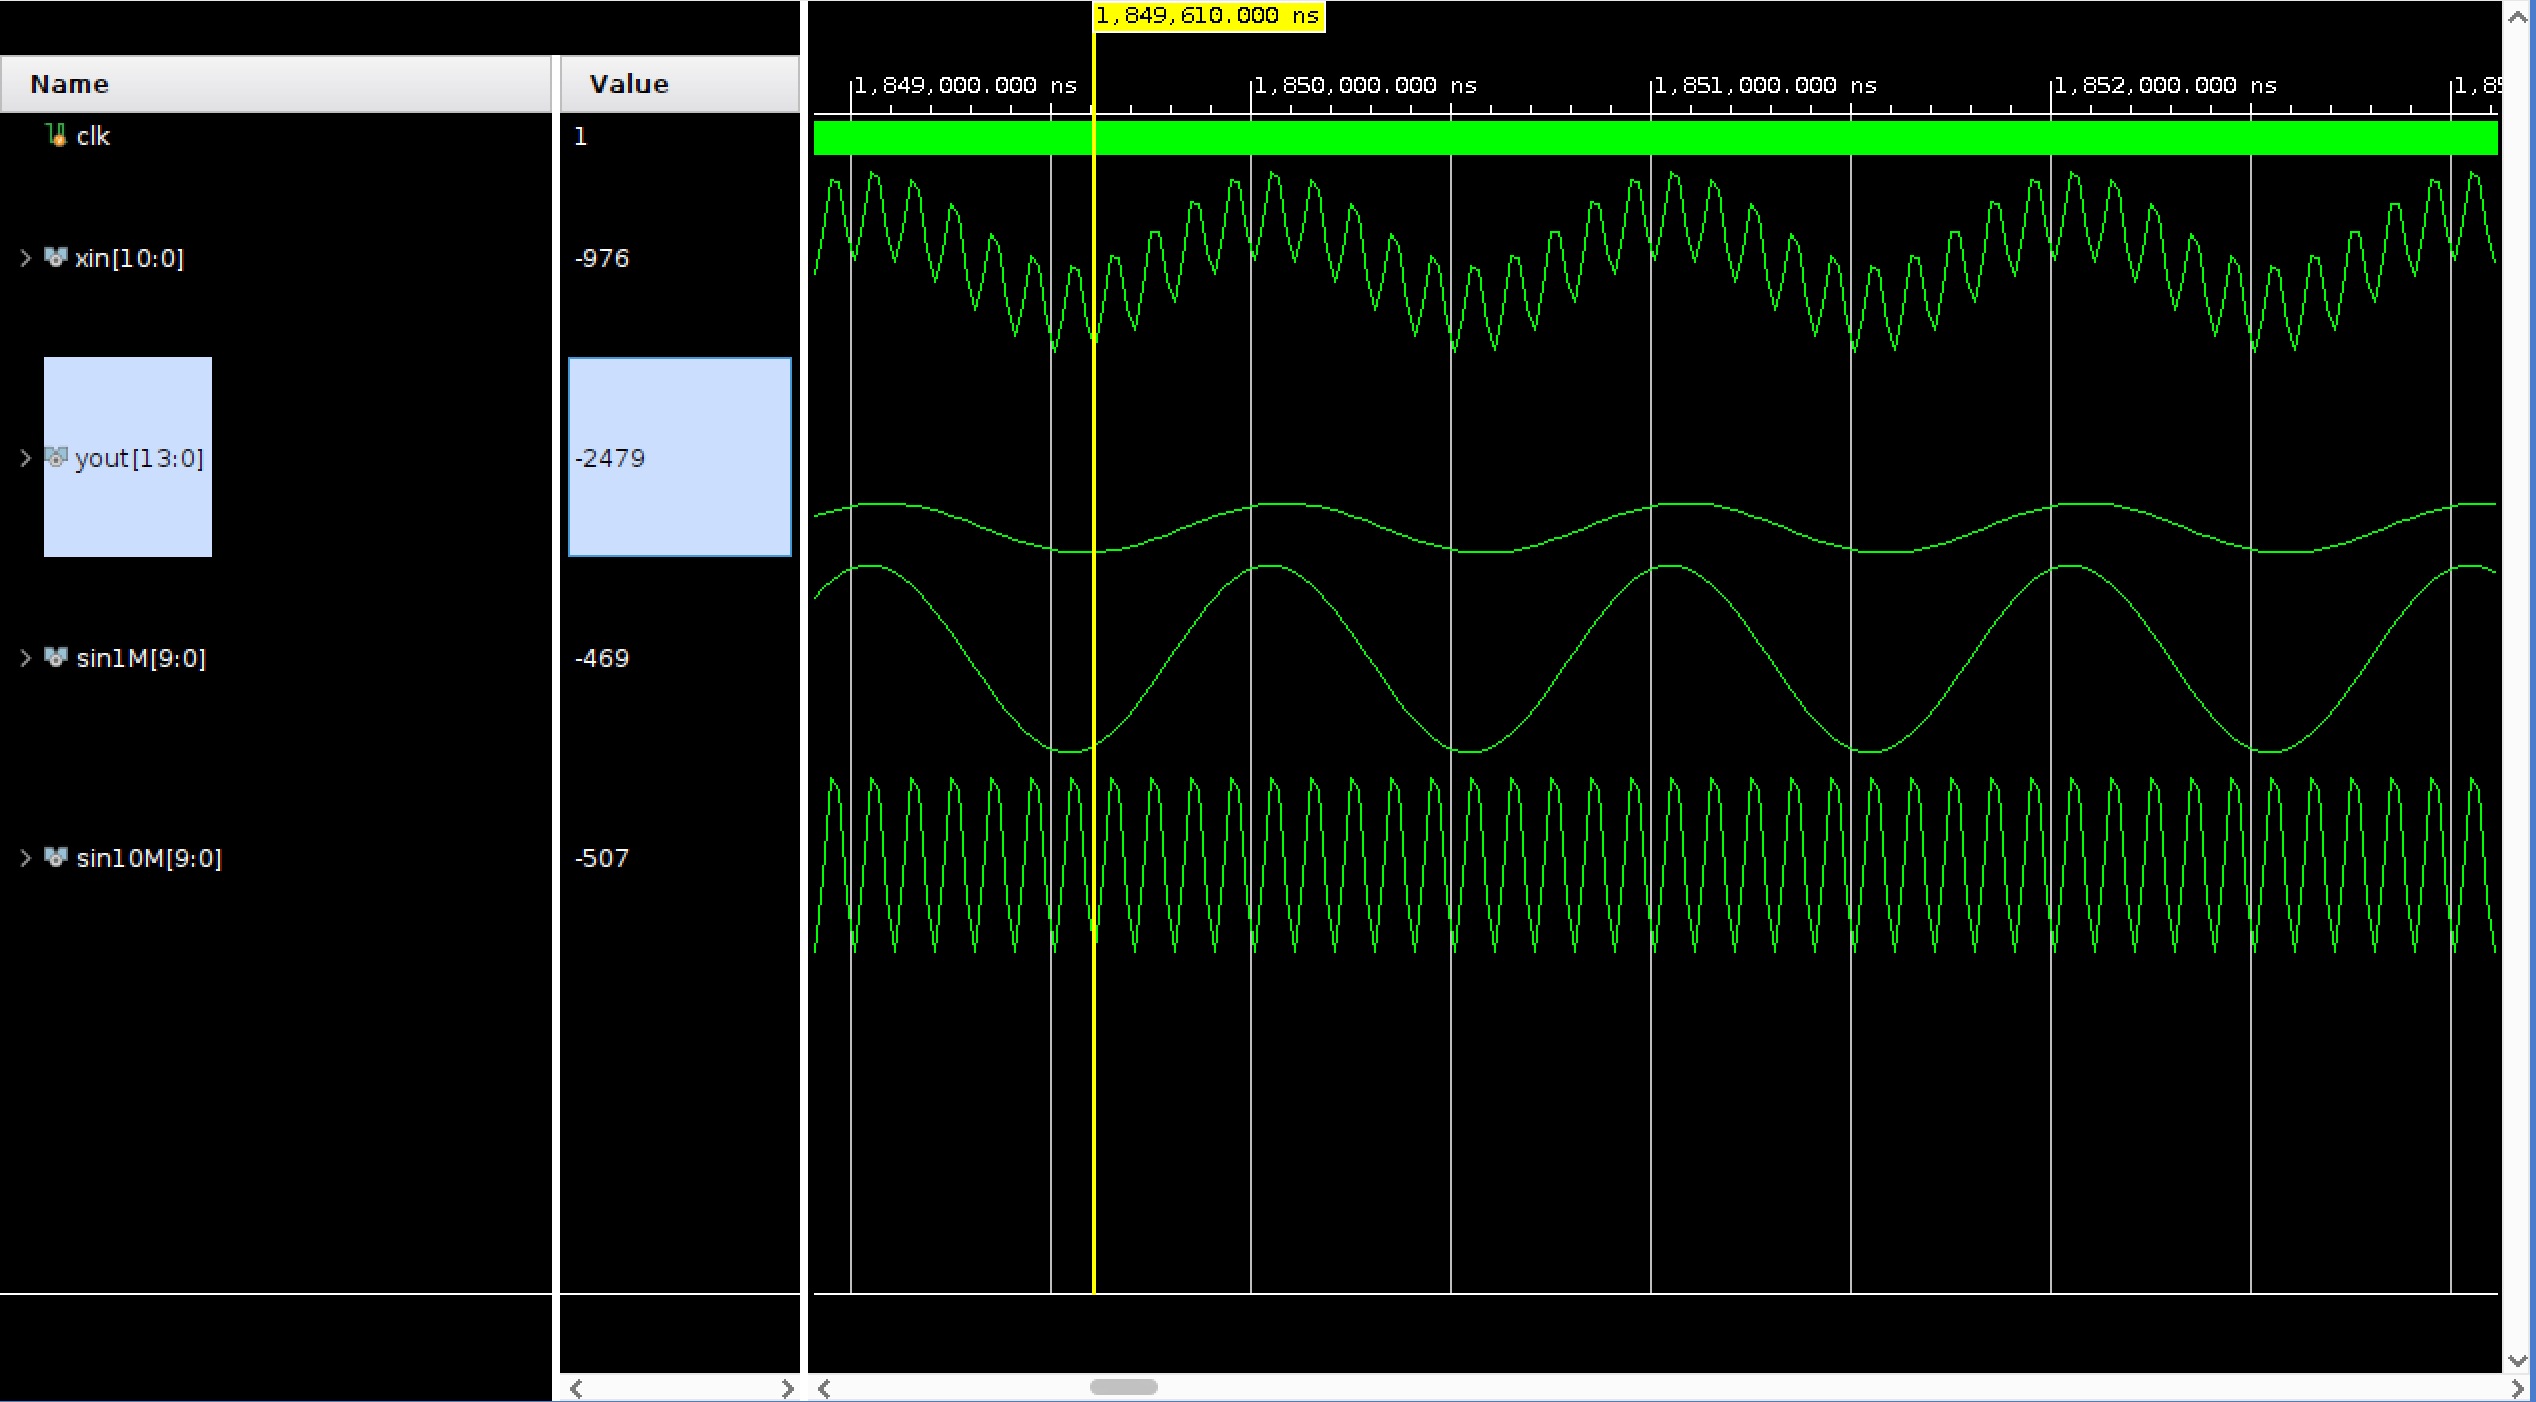
\includegraphics[width=0.75\textwidth]{figure/exp4/vivado_waveform.png}
  \caption{FIR滤波器滤波结果}
  \label{fig:exp4:result}
\end{figure}

为了进一步验证该模块的可靠性,将设计部署到FPGA上。在FIR模块之上,完成一个顶层模块,接口为FPGA(Zynq-7000)约束文件中的DAC接口。需要注意的是,该FPGA的时钟主频为100MHz,故需要调用\textit{Clocking Wizard}生成一个50MHz的时钟。该FPGA有两路DAC,故只能选择两路信号最终显示到示波器上,笔者选择滤波前和滤波后的两个信号。由于DAC的输出位宽为14,故对于不满14位的输入数据,按照二进制补码规则向上补齐符号位至14位。\footnote{在模拟域下,相当于幅度缩小16倍,但相对幅度是不变的。}代码如下。

\begin{lstlisting}[language=verilog,caption={顶层模块}]
  module TOP (
    PL_CLK_100MHz,
    LS_DAC2_DB,
    LS_DAC2_CLK,
    LS_DAC2_WRT,
    LS_DAC1_DB,
    LS_DAC1_CLK,
    LS_DAC1_WRT,
    LS_DAC_MODE
);
  // Inputs and Outputs
  input wire PL_CLK_100MHz;
  // board clock frequency = 100MHz, need to be written in tb


  // DAC Parameters
  output signed [13:0] LS_DAC2_DB;
  output LS_DAC2_CLK;
  output LS_DAC2_WRT;
  output signed [13:0] LS_DAC1_DB;
  output LS_DAC1_CLK;
  output LS_DAC1_WRT;
  output LS_DAC_MODE;


  wire clk;
  wire signed [13:0] fir_out;
  wire signed [9:0] sin_1M;
  wire signed [9:0] sin_10M;
  wire signed [10:0] sum;
  wire signed [13:0] sum_ext;
//   wire [15:0] sin_1M_temp;
//   wire [15:0] sin_10M_temp;

  // Clock IP: Generate 50MHz synchrous clk 
  CLK_50M module_clk_50M (
      // Clock out ports
      .clk_out1(clk),           // output clk_out1
      // Status and control signals
      .locked  (),              // output locked
      // Clock in ports
      .clk_in1 (PL_CLK_100MHz)  // input clk
  );



  SIN_1M module_sin_1M (
      .aclk                (clk),      // input wire aclk
      .s_axis_config_tvalid(1'b1),     // input wire s_axis_config_tvalid
      .s_axis_config_tdata (16'H51E),  // input wire [23 : 0] s_axis_config_tdata
      .m_axis_data_tvalid  (),         // output wire m_axis_data_tvalid
      .m_axis_data_tdata   (sin_1M)    // output wire [15 : 0] m_axis_data_tdata
  );

  SIN_10M module_sin_10M (
      .aclk                (clk),       // input wire aclk
      .s_axis_config_tvalid(1'b1),      // input wire s_axis_config_tvalid
      .s_axis_config_tdata (16'H3333),  // input wire [15 : 0] s_axis_config_tdata
      .m_axis_data_tvalid  (),          // output wire m_axis_data_tvalid
      .m_axis_data_tdata   (sin_10M)    // output wire [15 : 0] m_axis_data_tdata
  );

  FIR module_fir (
      .clk (clk),
      .xin (sum),     // 10 bits
      .yout(fir_out)  // 14 bits
  );

  // ILA Probe
  ILA module_probe (
      .clk(clk),  // input wire clk
      .probe0(sum_ext),  // 14 bits 
      .probe1(fir_out)  // 14 bits
  );


  // assignments

  assign sum         = sin_1M + sin_10M;  // auto truncate
  assign sum_ext     = {{3{sum[10]}}, sum};  // fill to 14 bits for output
//   assign sin_1M      = sin_1M_temp[15:6];
//   assign sin_10M     = sin_10M_temp[15:6];  // truncate only

  // DAC OUTPUT

  assign LS_DAC_MODE = 1'b1;
  assign LS_DAC1_DB  = sum_ext + 14'h2000;  // to unsigned data
  assign LS_DAC1_CLK = !clk;
  assign LS_DAC1_WRT = LS_DAC1_CLK;
  assign LS_DAC2_DB  = fir_out + 14'h2000;  // to unsigned data
  assign LS_DAC2_CLK = clk;
  assign LS_DAC2_WRT = LS_DAC2_CLK;

endmodule

\end{lstlisting}

生成TOP模块的比特流,并烧录到FPGA开发板上,可从ILA和示波器出看到波形(图~\ref{fig:exp4:Implementation})。
\begin{figure}[htbp]
  \centering
  \subfloat[滤波前(上)与滤波后(下)的ILA波形]{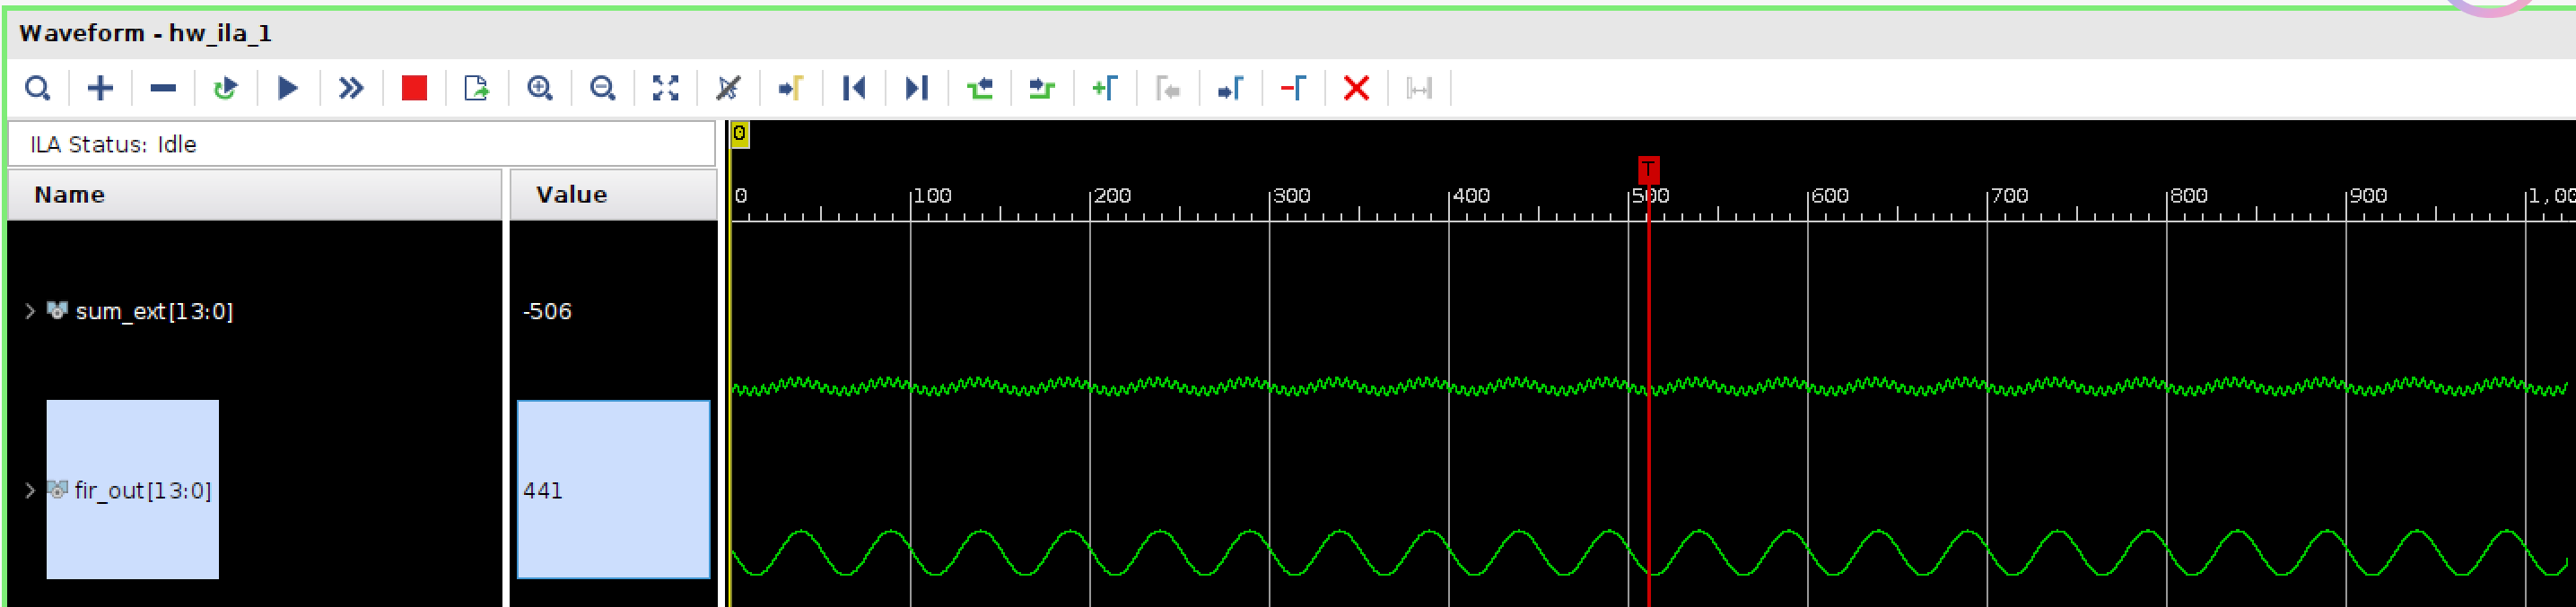
\includegraphics[width = 0.95\textwidth]{figure/exp4/waveform_ila.png}}
  \newline
  \subfloat[滤波前(黄色)与滤波后(绿色)的示波器波形]{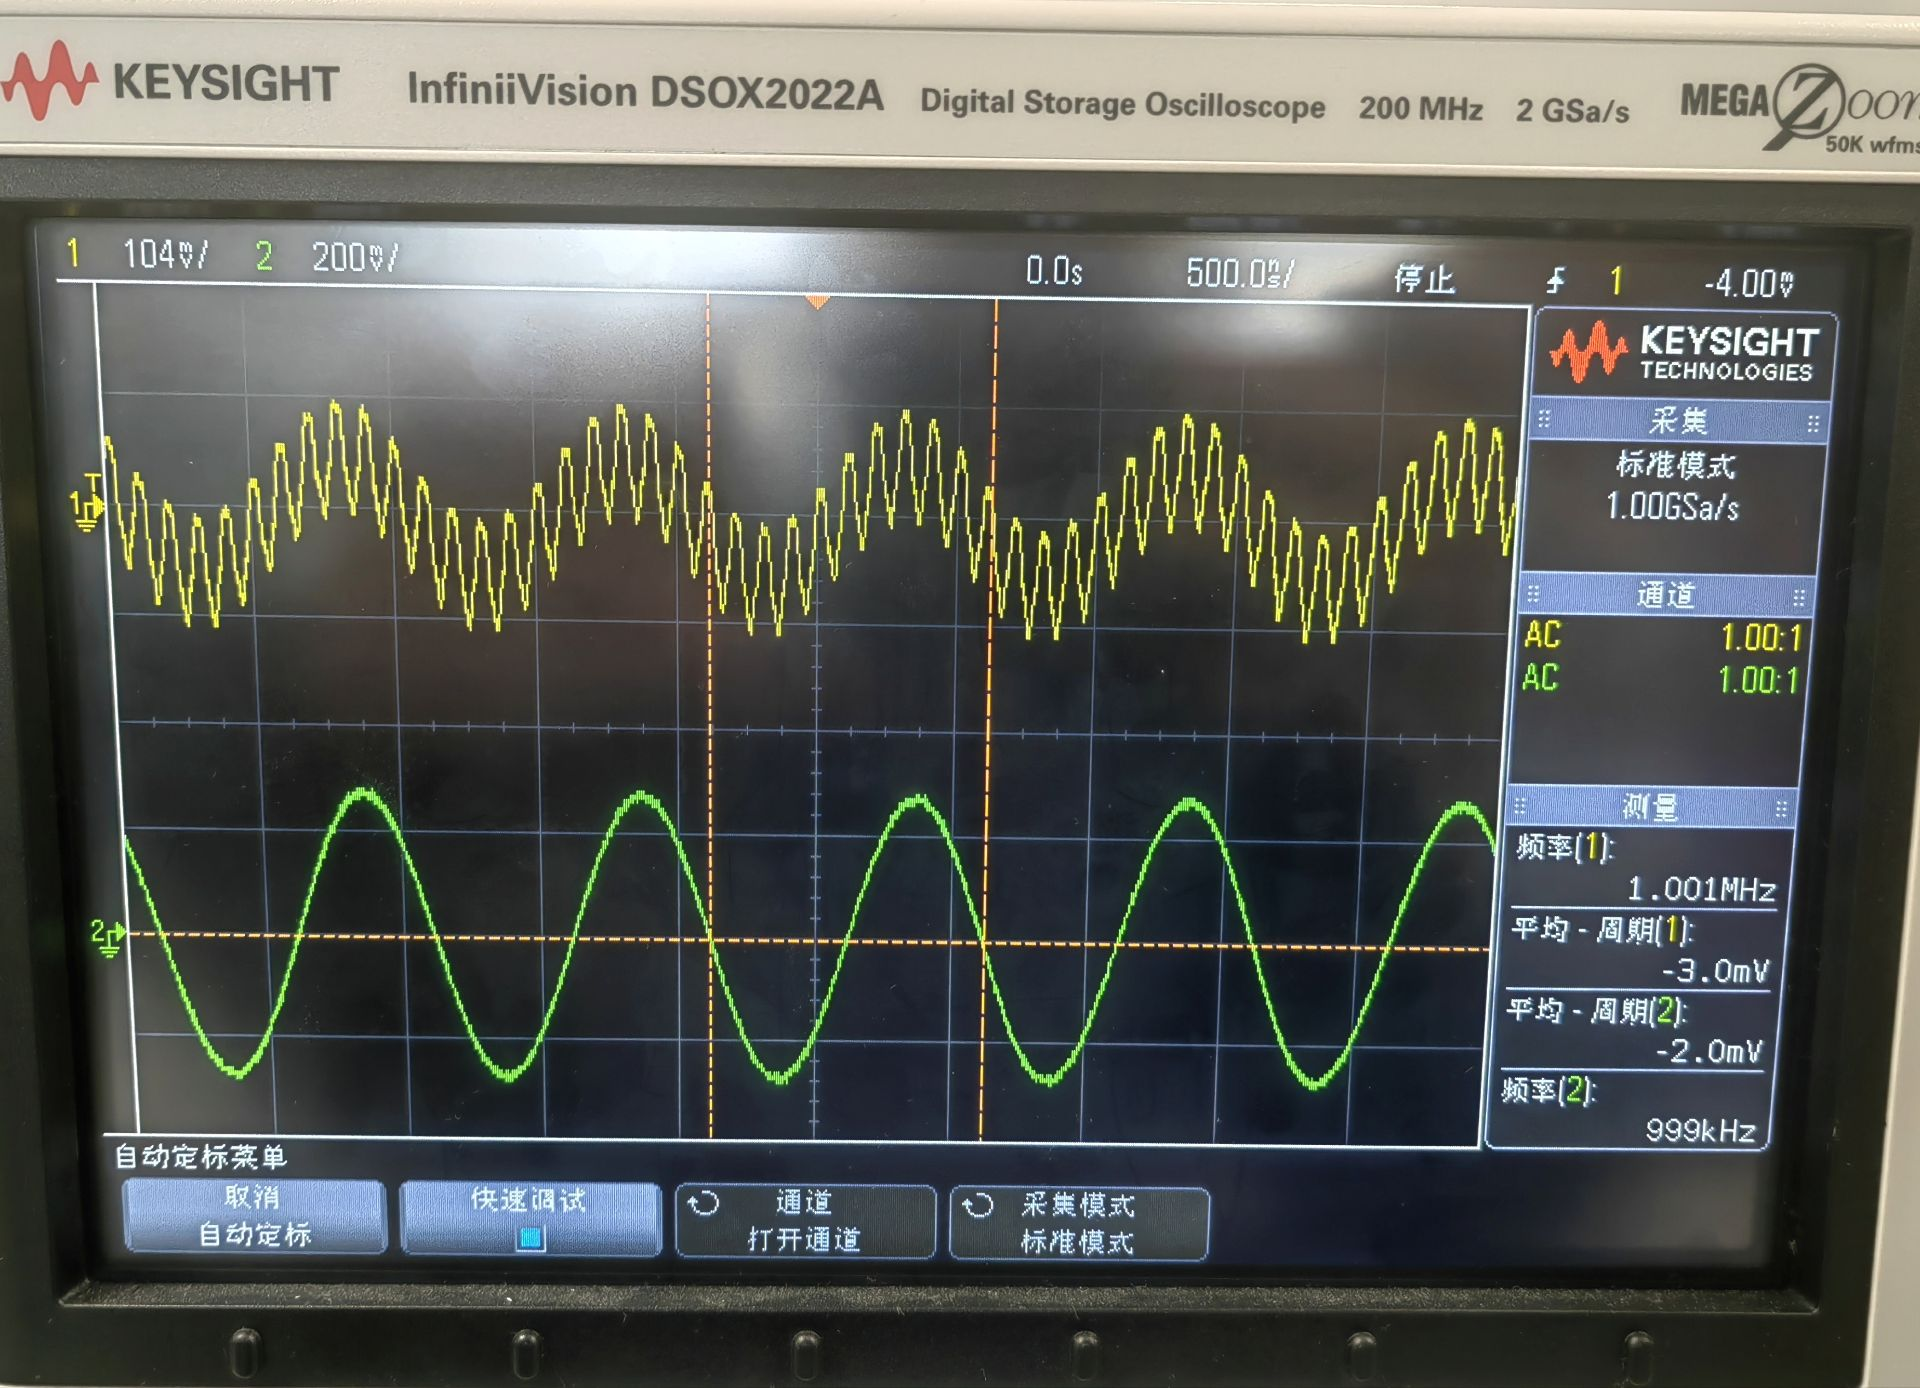
\includegraphics[width = 0.95\textwidth]{figure/exp4/waveform.jpg}}
  \caption{FPGA中滤波器输入输出的ILA与示波器波形}
  \label{fig:exp4:Implementation}
\end{figure}

\section{思考与讨论}
\subsection{更改参数的FIR滤波器实现}
更改FIR滤波器模块,使其适配公式~\ref{eqn:fir2}~的滤波器设置。
\begin{equation}\label{eqn:fir2}
  H(z) = 1 + 3z^{-1} + 2z^{-2} + 3z^{-3} + 2z^{-4} + 2.5z^{-5}
\end{equation}

注意到滤波器系数出现了小数,可以使用向右移位1位的方式构建0.5倍数。Verilog代码如下:
\begin{lstlisting}[language=verilog,caption={新版滤波器模块}]
module FIR_NEW (
    input                clk,  // 50MHz Clock
    input  signed [10:0] xin,  // input
    output signed [13:0] yout  // output
);

  reg signed [11:0] x1, x2, x3, x4, x5;  // cascaded registers
  always @(posedge clk) begin
    x1 <= xin;
    x2 <= x1;
    x3 <= x2;
    x4 <= x3;
    x5 <= x4;
  end

  // Output
  assign yout = xin + 3 * x1 + (x2 << 1) + 3 * x3 + (x4 << 1) + (x5 << 1) + (x5 >> 1);
endmodule

\end{lstlisting}

使用Testbench模块进行仿真,得到波形如图~\ref{fig:exp4:result2}。可以看到,波形相较均值滤波器,高频分量并未完全滤除。
\begin{figure}[htbp]
  \centering
  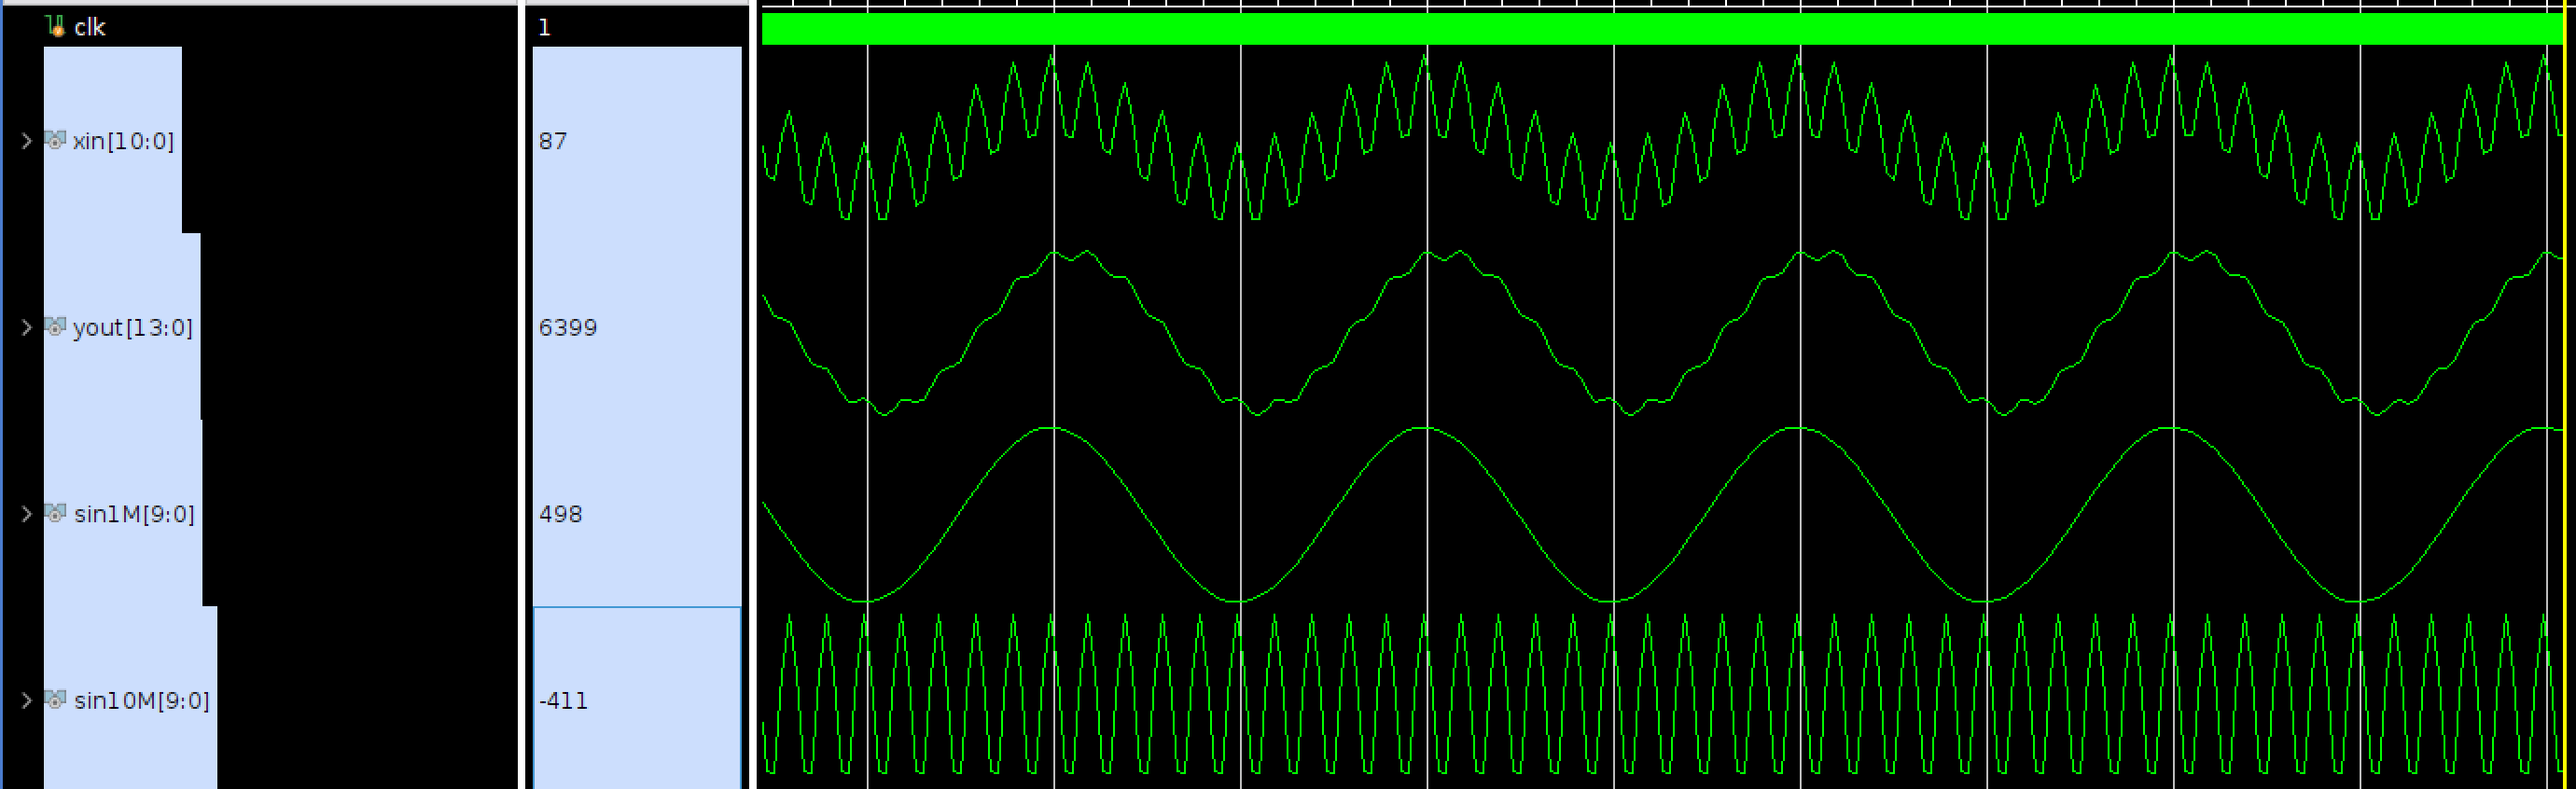
\includegraphics[width=0.75\textwidth]{figure/exp4/vivado_waveform_2.png}
  \caption{新版FIR滤波器滤波结果}
  \label{fig:exp4:result2}
\end{figure}

这是因为新版滤波器在高频下依然拥有比均值滤波器更高的频率响应(系数全正),导致高频分量与低频分量的差距减小。
\subsection{Linux系统下的 Vivado 配置}
FPGA的开发套件来源于芯片设计的开发套件,而绝大部分的芯片设计软件部署在Linux上。由此,Vivado作为典型的FPGA开发套件,可能也支持(甚至更适配)Linux开发环境。查阅资料可知,Vivado的Windows发行版(2021年)仍存在编译速度慢、工程代码同步、log打印占用时间/资源多等缺陷。因此,笔者将Vivado部署在Linux环境中后,完成了这次实验。安装的过程大量参考了\url{https://blog.csdn.net/weixin_46423500/article/details/142331804},将其重述如下。

使用Ubuntu24.04 Linux发行版进行环境配置。首先安装依赖:
\begin{lstlisting}[language=bash]
  sudo apt-get update
  sudo apt-get upgrade
  sudo apt-get install libncurses5
  sudo apt-get install libcanberra-gtk-module  
\end{lstlisting}

之后前往官网下载Vivado对应的Linux发行版。此过程需要在官网注册一个账号,该账号在随后的安装过程中仍然需要使用。下载完成后,执行下面的指令(\textbf{注意文件名要换成刚刚下载过的压缩包名字}。)
\begin{lstlisting}[language=bash]
  sudo chmod +x FPGAs_AdaptiveSoCs_Unified_version_info_Lin64.bin
  sudo sh ./FPGAs_AdaptiveSoCs_Unified_version_info_Lin64.bin
\end{lstlisting}

Vivado会自动执行安装程序。默认将在\texttt{tools/}下面安装Vivado。安装完成后,为了能够迅速从命令行启动vivado,需要在\texttt{./bashrc}文件夹下添加下面一行代码。
\begin{lstlisting}[language=bash]
  source tools/Xilinx/Vivado/2024.2/settings64.sh
\end{lstlisting}

可以通过gedit方式打开.bashrc。
\begin{lstlisting}[language=bash]
  sudo apt install gedit
  gedit .bashrc
\end{lstlisting}

至此,在命令行输入vivado即可打开GUI界面。另外,如果Linux安装语言并非英语,添加对英语的支持:
\begin{lstlisting}[language=bash]
  sudo locale-gen "en_US.UTF-8"
  sudo update-locale LANG=en_US.UTF-8
\end{lstlisting}

\subsection{Open Target时无法找到FPGA的解决办法}
本实验中,FPGA开发板与电脑通过JTAG接口连接。vivado在连接时可能由于软件或硬件原因显示不出FPGA开发板。对于硬件问题,通常可通过重新插拔或更换端口解决;但笔者在做实验的时候就遇到了软件上的问题:vivado在localhost上打开了一个端口用于硬件连接,接入JTAG-USB线后没有检测到任何硬件设备。

这种问题来源于电脑缺少JTAG驱动,需要手动(重新)安装。在Linux系统下,运行如下命令:
\begin{lstlisting}[language=bash]
  cd /YOUR_INSTALL_PATH/Xilinx/Vivado/YOUR_INSTALL_VERSION/data/xicom/cable_drivers/lin64/install_script/install_drivers
  sudo ./install_drivers
\end{lstlisting}

退出Vivado后重新打开便可正常识别。



% \chapter{并行结构的FIR滤波器设计}
\begin{introduction}
  \item \textit{乘法器IP核配置;}
  \item \textit{Verilog编写全并行结构FIR滤波器;}
  \item \textit{基于全并行结构的FIR滤波器FPGA实现。}
\end{introduction}
\section{实验背景与目的}
在现代数字信号处理(DSP)领域,FIR滤波器被广泛应用于信号的平滑、去噪、频率选择等任务。FIR滤波器的实现方式多种多样,基于FPGA(现场可编程门阵列)的实现因其并行处理能力和高效的硬件资源利用而成为常见的选择。本实验旨在通过基于FPGA的并行结构设计一个FIR滤波器,研究其实现过程并分析其资源消耗和时序性能。实验的主要目标是:
\begin{itemize}
    \item 设计并实现一个基于FPGA的并行结构FIR滤波器;
    \item 通过使用乘法器IP核优化滤波器的计算性能;
    \item 完成滤波器的FPGA实现,并进行资源消耗与时序性能的分析;
    \item 探讨如何提高该FIR滤波器的工作频率。
\end{itemize}

\section{实验原理}


\subsection{全并行结构FIR滤波器的实现}

在数字信号处理中,FIR滤波器是一种常用的线性时不变系统,能够有效地对输入信号进行滤波操作。为了提高处理速度并适应高速信号处理的需求,采用全并行结构实现FIR滤波器是一个有效的方式。在FPGA中实现全并行结构的FIR滤波器,主要包括以下几个部分:

\begin{enumerate}
    \item \textbf{输入数据存储}:输入信号 \( X[n] \) 被存储在一组移位寄存器中,这些寄存器按照时序顺序依次存储输入信号的历史样本数据。这些寄存器构成了滤波器的延迟单元。
    
    \item \textbf{加法器}:对于对称的滤波器系数,通过对称加法器对输入信号的不同延迟版本进行加和。这一操作减少了乘法器的使用,提高了设计效率。在实现中,通过多级加法器对输入信号进行并行加法处理。
    
    \item \textbf{乘法器}:每个加和后的输入信号与相应的滤波器系数 \( h[k] \) 进行乘法运算。为提高性能,设计中通常使用专用硬件乘法器,这些乘法器执行并行计算,处理每个延迟输入信号与滤波器系数的乘积。
    
    \item \textbf{加法汇总}:所有乘法结果通过加法器进行汇总,最终生成滤波器的输出。为了提高吞吐量,通常使用多级流水线加法器对乘法结果进行累加。
    
    \item \textbf{输出}:通过加法器的最终结果,获得滤波后的信号 \( Y[n] \),作为系统的输出。
\end{enumerate}

通过上述模块的并行实现,FIR滤波器能够在每个时钟周期内并行处理多个信号样本,从而大大提高了处理速度和效率。由于设计的FIR滤波器满足线性相位特性,因此可以省去一半的乘法器,进一步优化了硬件资源的利用。

\subsection{FPGA的主要资源}

FPGA(现场可编程门阵列)是一种灵活且高效的硬件平台,适用于多种数字电路设计。FPGA的主要资源包括:

\begin{enumerate}
    \item \textbf{查找表(LUTs,Look-Up Tables)}:用于实现基本的逻辑运算。LUT是FPGA的核心逻辑单元,通过查表的方式实现逻辑函数。复杂的逻辑操作会消耗更多的LUT资源。
    
    \item \textbf{寄存器(Registers)}:用于存储信号的状态,广泛应用于时序逻辑设计。每个寄存器通常需要一个时钟周期来更新其状态。
    
    \item \textbf{乘法器(Multipliers)}:硬件乘法器用于加速乘法运算。由于乘法是计算中最复杂的操作之一,FPGA提供专用的硬件乘法器以提高效率。
    
    \item \textbf{块RAM(Block RAM,BRAM)}:用于存储数据的内存资源,FPGA中提供多个BRAM块,可用于存储大量数据,如滤波器的中间计算结果。
    
    \item \textbf{时钟资源}:FPGA内部包含多个时钟源,用于驱动不同的时钟域。时钟设计在FPGA中非常重要,合理的时钟管理可以优化系统性能。
    
    \item \textbf{输入输出引脚(I/O Pins)}:FPGA通过I/O引脚与外部世界进行数据交换,设计中的I/O需求会消耗一定的资源。
    
    \item \textbf{逻辑块(Logic Blocks)}:每个FPGA包含多个逻辑块,通常由多个LUT、寄存器和其他功能单元组成。设计时的逻辑块使用量直接影响FPGA的资源消耗。
\end{enumerate}

\subsection{时序与资源分析的重要性}

时序和资源分析是FPGA设计过程中不可或缺的一部分,其重要性体现在以下几个方面:

\begin{enumerate}
    \item \textbf{时序分析}:时序分析确保设计满足时钟约束,即确保设计中的信号在正确的时钟边缘触发,并且信号能够在规定的时间内稳定。时序问题可能导致信号错误传输,从而影响系统的正常运行。通过时序分析,可以识别设计中存在的潜在时序问题,如时序余量不足、时钟频率限制等问题,并采取措施进行优化。
    
    \item \textbf{资源分析}:FPGA的资源有限,设计中不同模块会消耗不同类型的资源(如LUT、寄存器、BRAM等)。资源消耗分析能够帮助设计者了解设计中哪些部分消耗了大量资源,从而采取优化措施。例如,可以通过减少不必要的逻辑单元、使用更高效的算法或者共享资源来减少FPGA资源的占用,降低功耗并提高系统性能。
    
    \item \textbf{优化设计}:通过时序和资源分析,设计者可以识别瓶颈,并采取相应的优化措施。例如,时序优化可能包括调整时钟频率、使用更高效的时钟分配方案;资源优化可能包括使用更紧凑的算法、共享硬件资源或将设计分割成多个模块,以便在不同的FPGA资源中均匀分配。
\end{enumerate}

综上所述,时序和资源分析不仅能够确保设计的正确性,还能帮助设计者有效地利用FPGA资源,最大化其性能并降低系统的成本。

\section{实验使用软件/平台}
\begin{itemize}
  \item Xilinx Vivado 2024.2;
  \item eNodeX 30B软件无线电创新平台;
  \item 示波器。
  \item MATLAB \& Simulink R2024b;
\end{itemize}
\section{实验内容}
\subsection{乘法器IP核配置}
在本例中,生成的FIR滤波器系数为12位有符号数,而待滤波数据经过对称相加后,需要支持13位有符号数。因此需要例化一个$13\times 12$的有符号数乘法器。由于不需要设计流水线,故对乘法器没有控制要求,因此取消同步控制信号和时钟Enable信号,降低设计复杂度。乘法器配置如图~\ref{fig:exp5:mult}。
\begin{figure}[htbp]
  \centering
  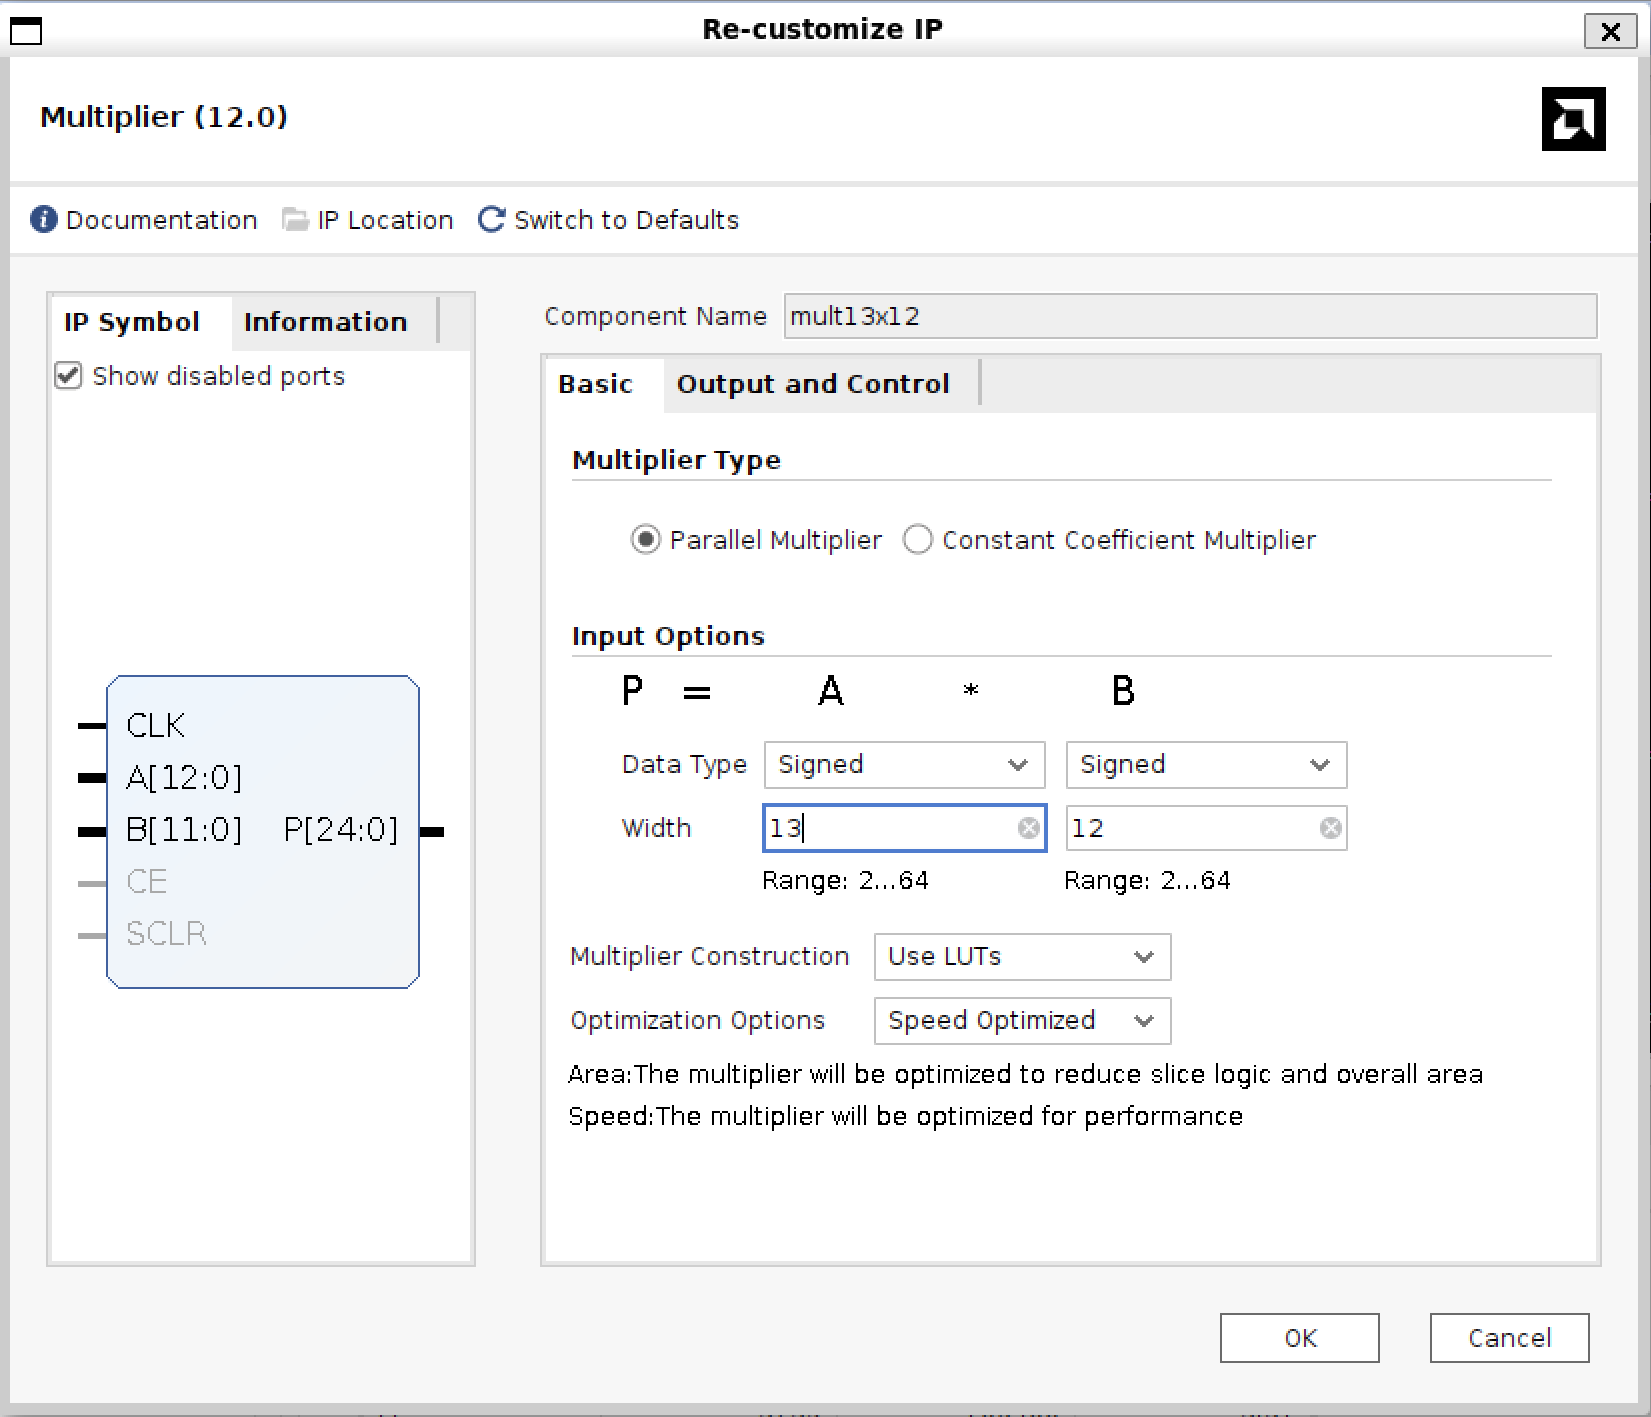
\includegraphics[width=0.75\textwidth]{figure/exp5/mult_settings.png}
  \caption{乘法器配置}
  \label{fig:exp5:mult}
\end{figure}

\subsection{全并行结构FIR滤波器的FPGA实现}
设计一个全并行的FIR滤波器,其输入输出端口如表~\ref{table:interface_fir_exp5}~所示。由于引入乘法器,输出信号位宽约为输入信号位宽的2倍。

\begin{table}[htbp]
  \centering
  \begin{tabular}{ccc}
    \toprule
     信号名 & 意义 & 端口类型\\
    \midrule
      \texttt{clk} & 50MHz时钟信号 & Input \\
     \texttt{Xin} & 12-bit 加和后量化正弦信号 & Input \\
     \texttt{Yout} & 26-bit 滤波后量化信号输出 & Output \\
    \bottomrule
  \end{tabular}
  \caption{FIR模块接口说明}
  \label{table:interface_fir_exp5}
\end{table}

下面的Verilog模块实现了一个全并行、全展开的FIR滤波器。输入信号 \texttt{Xin} 被存储在16个寄存器中,之后通过加法器对称相加。利用8个乘法器与MATLAB计算好的滤波器系数进行乘法运算,并通过两级流水线对结果进行加法汇总,最终输出滤波结果 \texttt{Yout}。

\begin{remark}
  \kaishu{由于该滤波器$N$为偶数且接近偶对称,故可以推断其为低通或带通滤波器,如设计好均可滤除8MHz的高频信号。}
\end{remark}
\begin{lstlisting}[language=verilog,caption={FIR滤波器模块}]
  `timescale 1ns / 1ps
  module fir_parallel( 
      input clk,            // 系统时钟
      input signed [11:0] Xin, // 输入数据
      output signed [25:0] Yout // 输出数据
  );
  
      // 定义滤波器系数
      parameter signed [11:0] coeff_b0 = -12'd116;
      parameter signed [11:0] coeff_b1 = -12'd111;
      parameter signed [11:0] coeff_b2 = -12'd22;
      parameter signed [11:0] coeff_b3 = 12'd243;
      parameter signed [11:0] coeff_b4 = 12'd692;
      parameter signed [11:0] coeff_b5 = 12'd1239;
      parameter signed [11:0] coeff_b6 = 12'd1743;
      parameter signed [11:0] coeff_b7 = 12'd2047;
  
      // 将数据存入移位寄存器Xin_Reg中
      reg signed [11:0] Xin_Reg[15:0];
      always @(posedge clk) begin
          Xin_Reg[0] <= Xin;
          Xin_Reg[1] <= Xin_Reg[0];
          Xin_Reg[2] <= Xin_Reg[1];
          Xin_Reg[3] <= Xin_Reg[2];
          Xin_Reg[4] <= Xin_Reg[3];
          Xin_Reg[5] <= Xin_Reg[4];
          Xin_Reg[6] <= Xin_Reg[5];
          Xin_Reg[7] <= Xin_Reg[6];
          Xin_Reg[8] <= Xin_Reg[7];
          Xin_Reg[9] <= Xin_Reg[8];
          Xin_Reg[10] <= Xin_Reg[9];
          Xin_Reg[11] <= Xin_Reg[10];
          Xin_Reg[12] <= Xin_Reg[11];
          Xin_Reg[13] <= Xin_Reg[12];
          Xin_Reg[14] <= Xin_Reg[13];
          Xin_Reg[15] <= Xin_Reg[14];
      end
  
      // 采用8个双输入加法器,完成对称系数相加
      // 两个12比特数据相加,需要用13比特数据存储数据
      reg signed [12:0] Xin_Add [7:0];
      always @(posedge clk) begin
          Xin_Add[0] = Xin_Reg[0] + Xin_Reg[15];
          Xin_Add[1] = Xin_Reg[1] + Xin_Reg[14];
          Xin_Add[2] = Xin_Reg[2] + Xin_Reg[13];
          Xin_Add[3] = Xin_Reg[3] + Xin_Reg[12];
          Xin_Add[4] = Xin_Reg[4] + Xin_Reg[11];
          Xin_Add[5] = Xin_Reg[5] + Xin_Reg[10];
          Xin_Add[6] = Xin_Reg[6] + Xin_Reg[9];
          Xin_Add[7] = Xin_Reg[7] + Xin_Reg[8];
      end
  
      // 实例化8个有符号数乘法器IP核mult,
      // 1级流水线延时输出
      wire signed [24:0] Mout [7:0];
      mult13x12 u0 (.CLK(clk), .A(Xin_Add[0]), .B(coeff_b0), .P(Mout[0]));
      mult13x12 u1 (.CLK(clk), .A(Xin_Add[1]), .B(coeff_b1), .P(Mout[1]));
      mult13x12 u2 (.CLK(clk), .A(Xin_Add[2]), .B(coeff_b2), .P(Mout[2]));
      mult13x12 u3 (.CLK(clk), .A(Xin_Add[3]), .B(coeff_b3), .P(Mout[3]));
      mult13x12 u4 (.CLK(clk), .A(Xin_Add[4]), .B(coeff_b4), .P(Mout[4]));
      mult13x12 u5 (.CLK(clk), .A(Xin_Add[5]), .B(coeff_b5), .P(Mout[5]));
      mult13x12 u6 (.CLK(clk), .A(Xin_Add[6]), .B(coeff_b6), .P(Mout[6]));
      mult13x12 u7 (.CLK(clk), .A(Xin_Add[7]), .B(coeff_b7), .P(Mout[7]));
  
      // 采用2级流水线完成8输入加法运算
      reg signed [26:0] sum1, sum2;
      reg signed [27:0] sum;
      always @(posedge clk) begin
          sum1 <= Mout[0] + Mout[1] + Mout[2] + Mout[3];
          sum2 <= Mout[4] + Mout[5] + Mout[6] + Mout[7];
          sum <= sum1 + sum2;
      end
  
      assign Yout = sum[25:0];
  
  endmodule
  \end{lstlisting}

基于此模块设计,编写测试模块(Testbench)如下。在测试模块中调用\textit{DDS Compiler} IP核生成1MHz和8MHz的正弦信号并相加后,对FIR模块进行测试。
\begin{lstlisting}[language=verilog, caption={Testbench文件}]
  `timescale 1ns / 1ps

module tb_FIR_PARALLEL;

    reg clk; // 时钟信号
    wire signed [11:0] xin; // FIR 输入信号
    wire signed [25:0] yout; // FIR 输出信号
    wire signed [11:0] sin1M, sin8M; // DDS 产生的两个输入信号

    fir_parallel sim (
        .clk(clk),
        .Xin(xin),  // 确保正确连接输入信号
        .Yout(yout) // 确保正确连接输出信号
    );

    // 产生 50MHz 的时钟信号
    initial begin
        clk = 0;
        forever #10 clk = ~clk;
    end

    // 实例化 SIN_1M 模块
    SIN_1M sin_1M (
        .aclk(clk),                                  // 输入时钟信号
        .s_axis_config_tvalid(1'b1),  // 配置有效信号
        .s_axis_config_tdata(16'H51E),    // 配置数据
        .m_axis_data_tvalid(),      // 数据有效信号
        .m_axis_data_tdata(sin1M)        // 输出数据
    );

    // 实例化 SIN_8M 模块
    SIN_8M sin_8M (
        .aclk(clk),                                  // 输入时钟信号
        .s_axis_config_tvalid(1'b1),  // 配置有效信号
        .s_axis_config_tdata(16'H28F5),    // 配置数据
        .m_axis_data_tvalid(),      // 数据有效信号
        .m_axis_data_tdata(sin8M)        // 输出数据
    );

    // 计算输入信号 xin
    assign xin = sin1M + sin8M;  // 将两个信号相加作为 FIR 输入信号

endmodule

  
\end{lstlisting}

测试结果如图~\ref{fig:exp5:result}~所示。\footnote{需要在xsim中调整数据格式(Radix)为Signed Decimal,波形格式为Analog。}可以看出设计的FIR滤波器成功滤除了高频的8MHz信号,而保留了1MHz的信号,这符合低通滤波器的特性。
\begin{figure}[htbp]
  \centering
  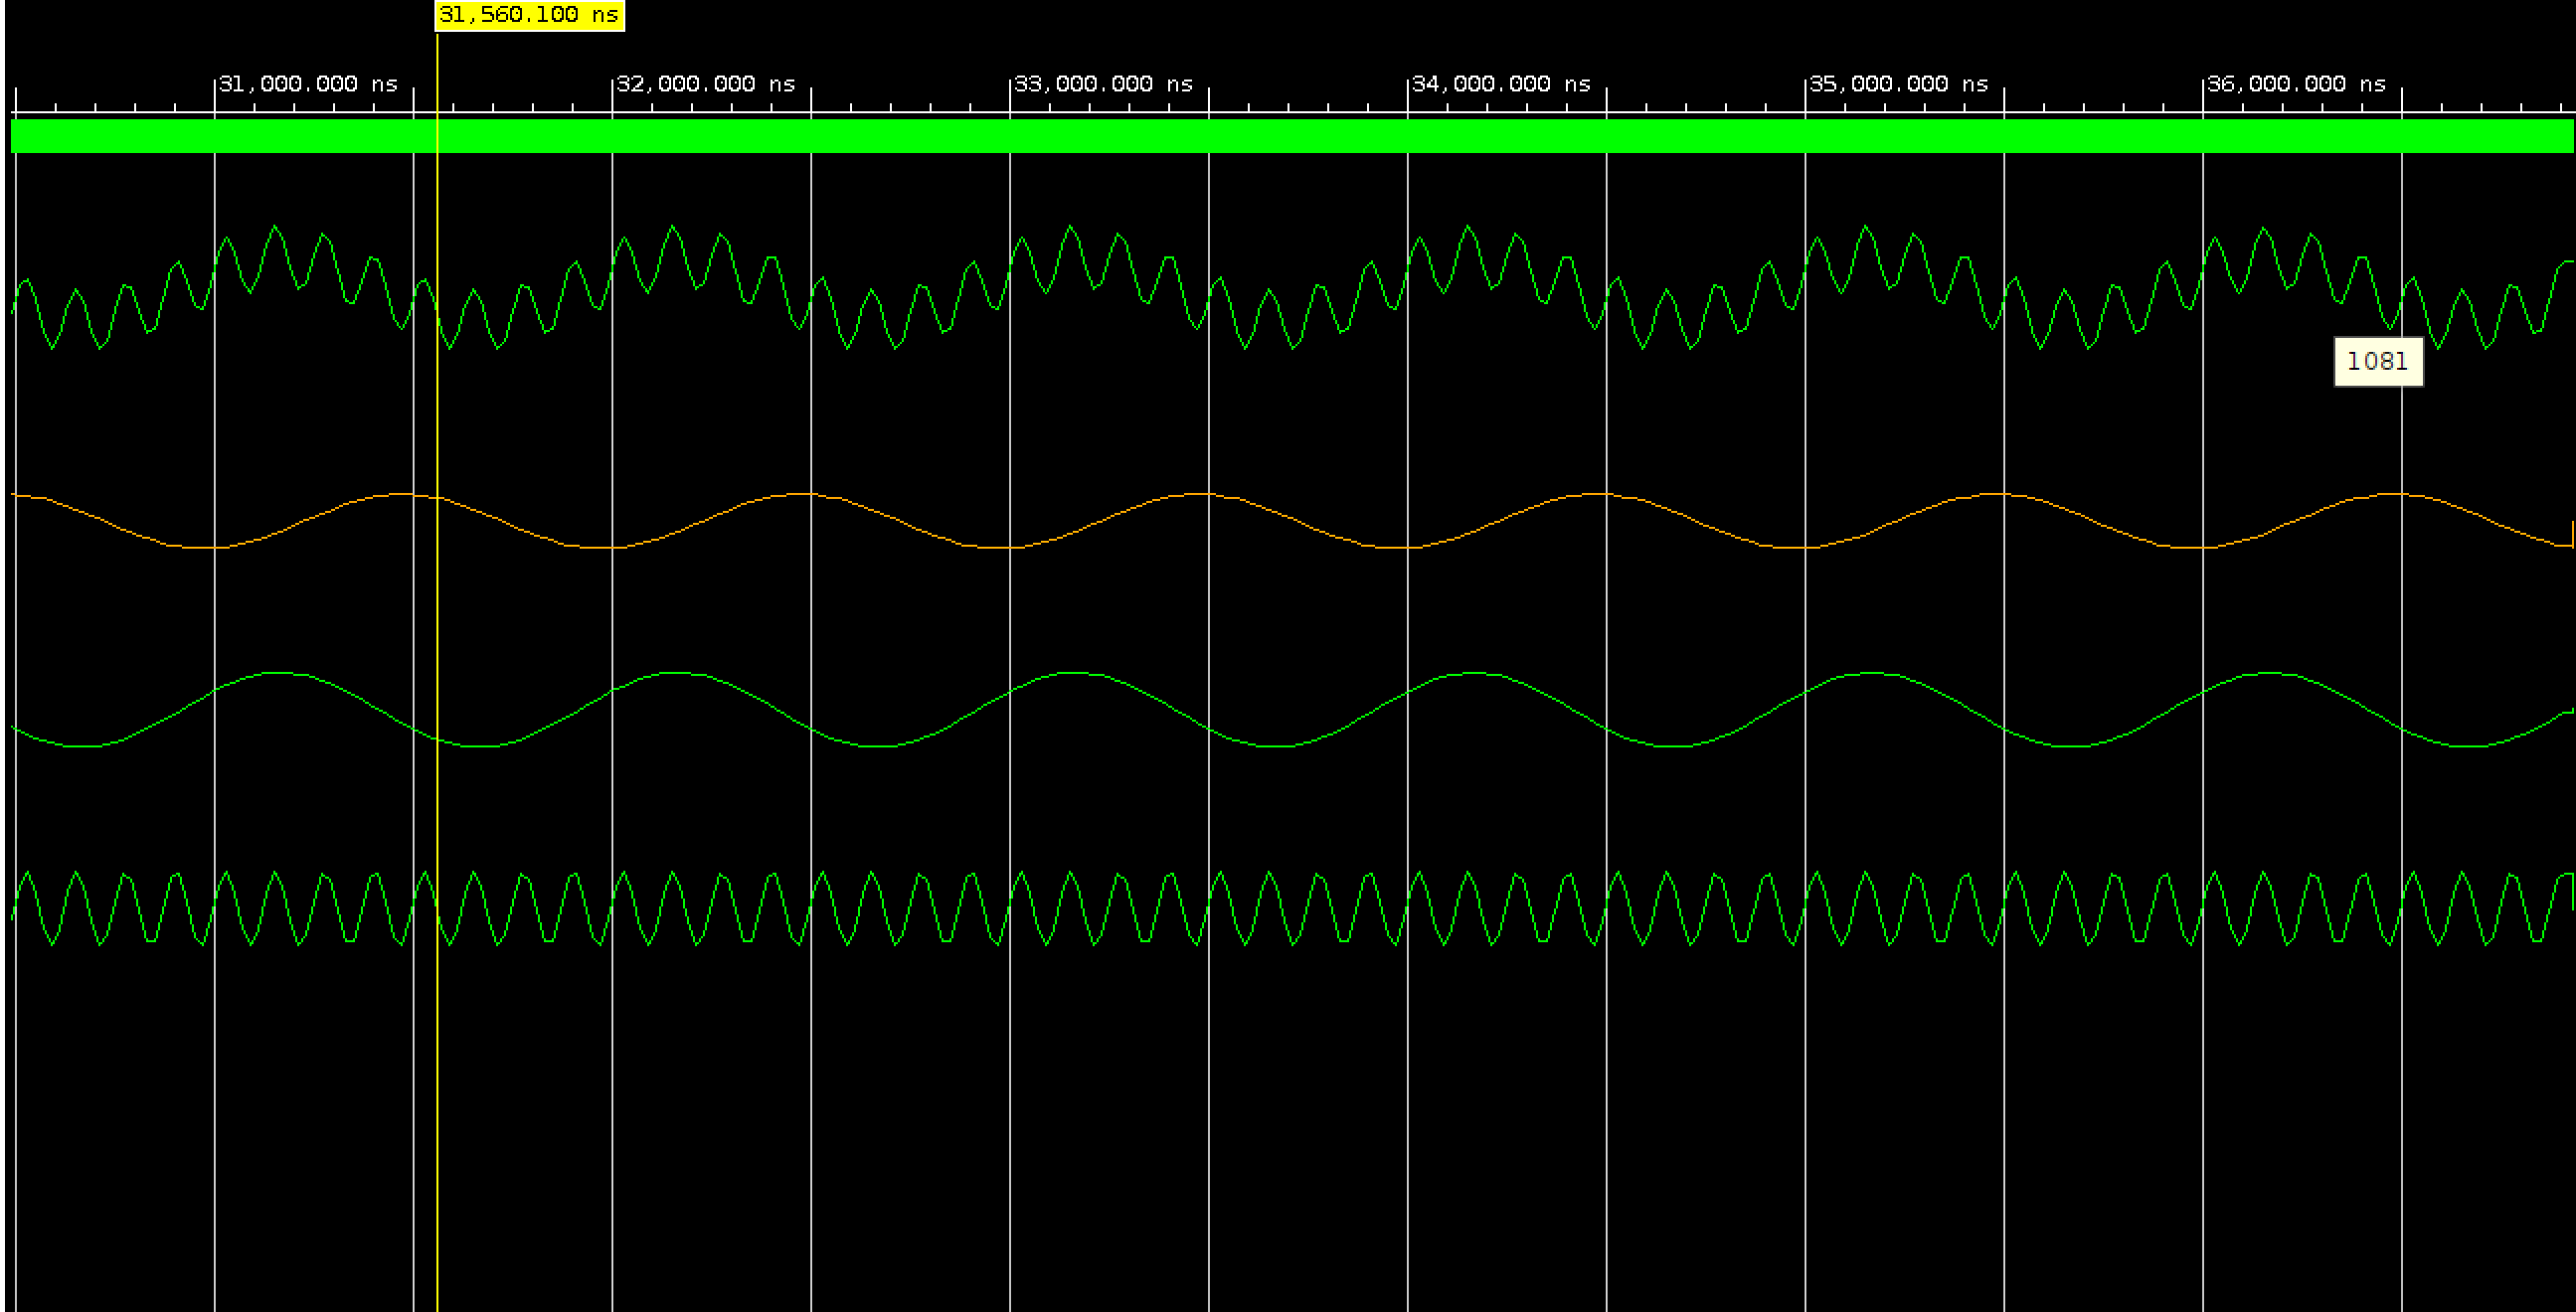
\includegraphics[width=0.75\textwidth]{figure/exp5/waveform.png}
  \caption{FIR滤波器滤波结果}
  \label{fig:exp5:result}
\end{figure}

为了进一步验证该模块的可靠性,将设计部署到FPGA上。在FIR模块之上,复用上一章的顶层模块,并选择滤波前和滤波后的两个信号。由于DAC的输出位宽为14,故对于不满14位的输入数据,按照二进制补码规则向上补齐符号位至14位。\footnote{在模拟域下,相当于幅度缩小16倍,但相对幅度是不变的。}而对大于14位的信号,则选择最高14位(含符号位)截断,舍弃低位。代码如下。

\begin{lstlisting}[language=verilog,caption={顶层模块}]
`timescale 1ns / 1ps
module TOP (
    // DAC  PINS
    output signed [13:0] LS_DAC2_DB,   // DA 数据2
    output               LS_DAC2_CLK,  // DA 时钟2 (125MHz 以下)
    output               LS_DAC2_WRT,  // DA 输出写信号,同时钟信号
    output signed [13:0] LS_DAC1_DB,   // DA 数据1
    output               LS_DAC1_CLK,  // DA 时钟1 (125MHz 以下)
    output               LS_DAC1_WRT,  // DA 输出写信号,同时钟信号

    output LS_DAC_MODE,     

    input PL_CLK_100MHz  // 时钟输入
);

  wire               clk_50M;
  wire               clk_locked;
  wire signed [10:0] sin8M;
  wire signed [10:0] sin1M;
  wire signed [11:0] xin;  //重新定义了两个端口
  wire signed [13:0] xin_new;
  wire signed [25:0] yout;
  clk50m inst_clk50m (
      // Clock out ports
      .clk_out_50m(clk_50M),       // output clk_out_50m
      // Status and control signals
      .locked     (clk_locked),    // output locked
      // Clock in ports
      .clk_in1    (PL_CLK_100MHz)  // input clk_in1
  );

  ila_0 inst_ila (
      .clk(clk_50M),  // input wire clk
      .probe0(xin_new),  // input wire [13:0]  probe0 ,修改为11位 
      .probe1(yout[25:12])  // input wire [13:0]  probe1
  );


  fir_parallel sim (
      .clk(clk_50M),
      .Xin(xin),  // 确保正确连接输入信号
      .Yout(yout)  // 确保正确连接输出信号
  );

  SIN_1M sin_1M (
      .aclk                (clk_50M),  // input wire aclk
      .s_axis_config_tvalid(1'b1),     // input wire s_axis_config_tvalid
      .s_axis_config_tdata (16'H51E),  // input wire [11 : 0] s_axis_config_tdata
      .m_axis_data_tvalid  (),         // output wire m_axis_data_tvalid
      .m_axis_data_tdata   (sin1M)     // output wire [11 : 0] m_axis_data_tdata
  );
  SIN_8M sin_8M (
      .aclk                (clk_50M),   // input wire aclk
      .s_axis_config_tvalid(1'b1),      // input wire s_axis_config_tvalid
      .s_axis_config_tdata (16'H28F5),  // input wire [15 : 0] s_axis_config_tdata
      .m_axis_data_tvalid  (),          // output wire m_axis_data_tvalid
      .m_axis_data_tdata   (sin8M)     // output wire [15 : 0] m_axis_data_tdata
  );

  // 计算输入信号
  assign xin = sin1M + sin8M;
  assign xin_new = {{2{xin[11]}}, xin};  //完成位数的扩展
  // DAC OUTPUT
  assign LS_DAC_MODE = 1'b1;
  assign LS_DAC1_DB = xin_new + 14'h2000;  
  assign LS_DAC1_CLK = !clk_50M;
  assign LS_DAC1_WRT = LS_DAC1_CLK;
  assign LS_DAC2_DB = yout[25:12] + 14'h2000;  //位宽
  assign LS_DAC2_CLK = clk_50M;
  assign LS_DAC2_WRT = LS_DAC2_CLK;

endmodule


\end{lstlisting}

生成TOP模块的比特流,并烧录到FPGA开发板上,可从示波器处看到波形(图~\ref{fig:exp5:Implementation})。
\begin{figure}[htbp]
  \centering
  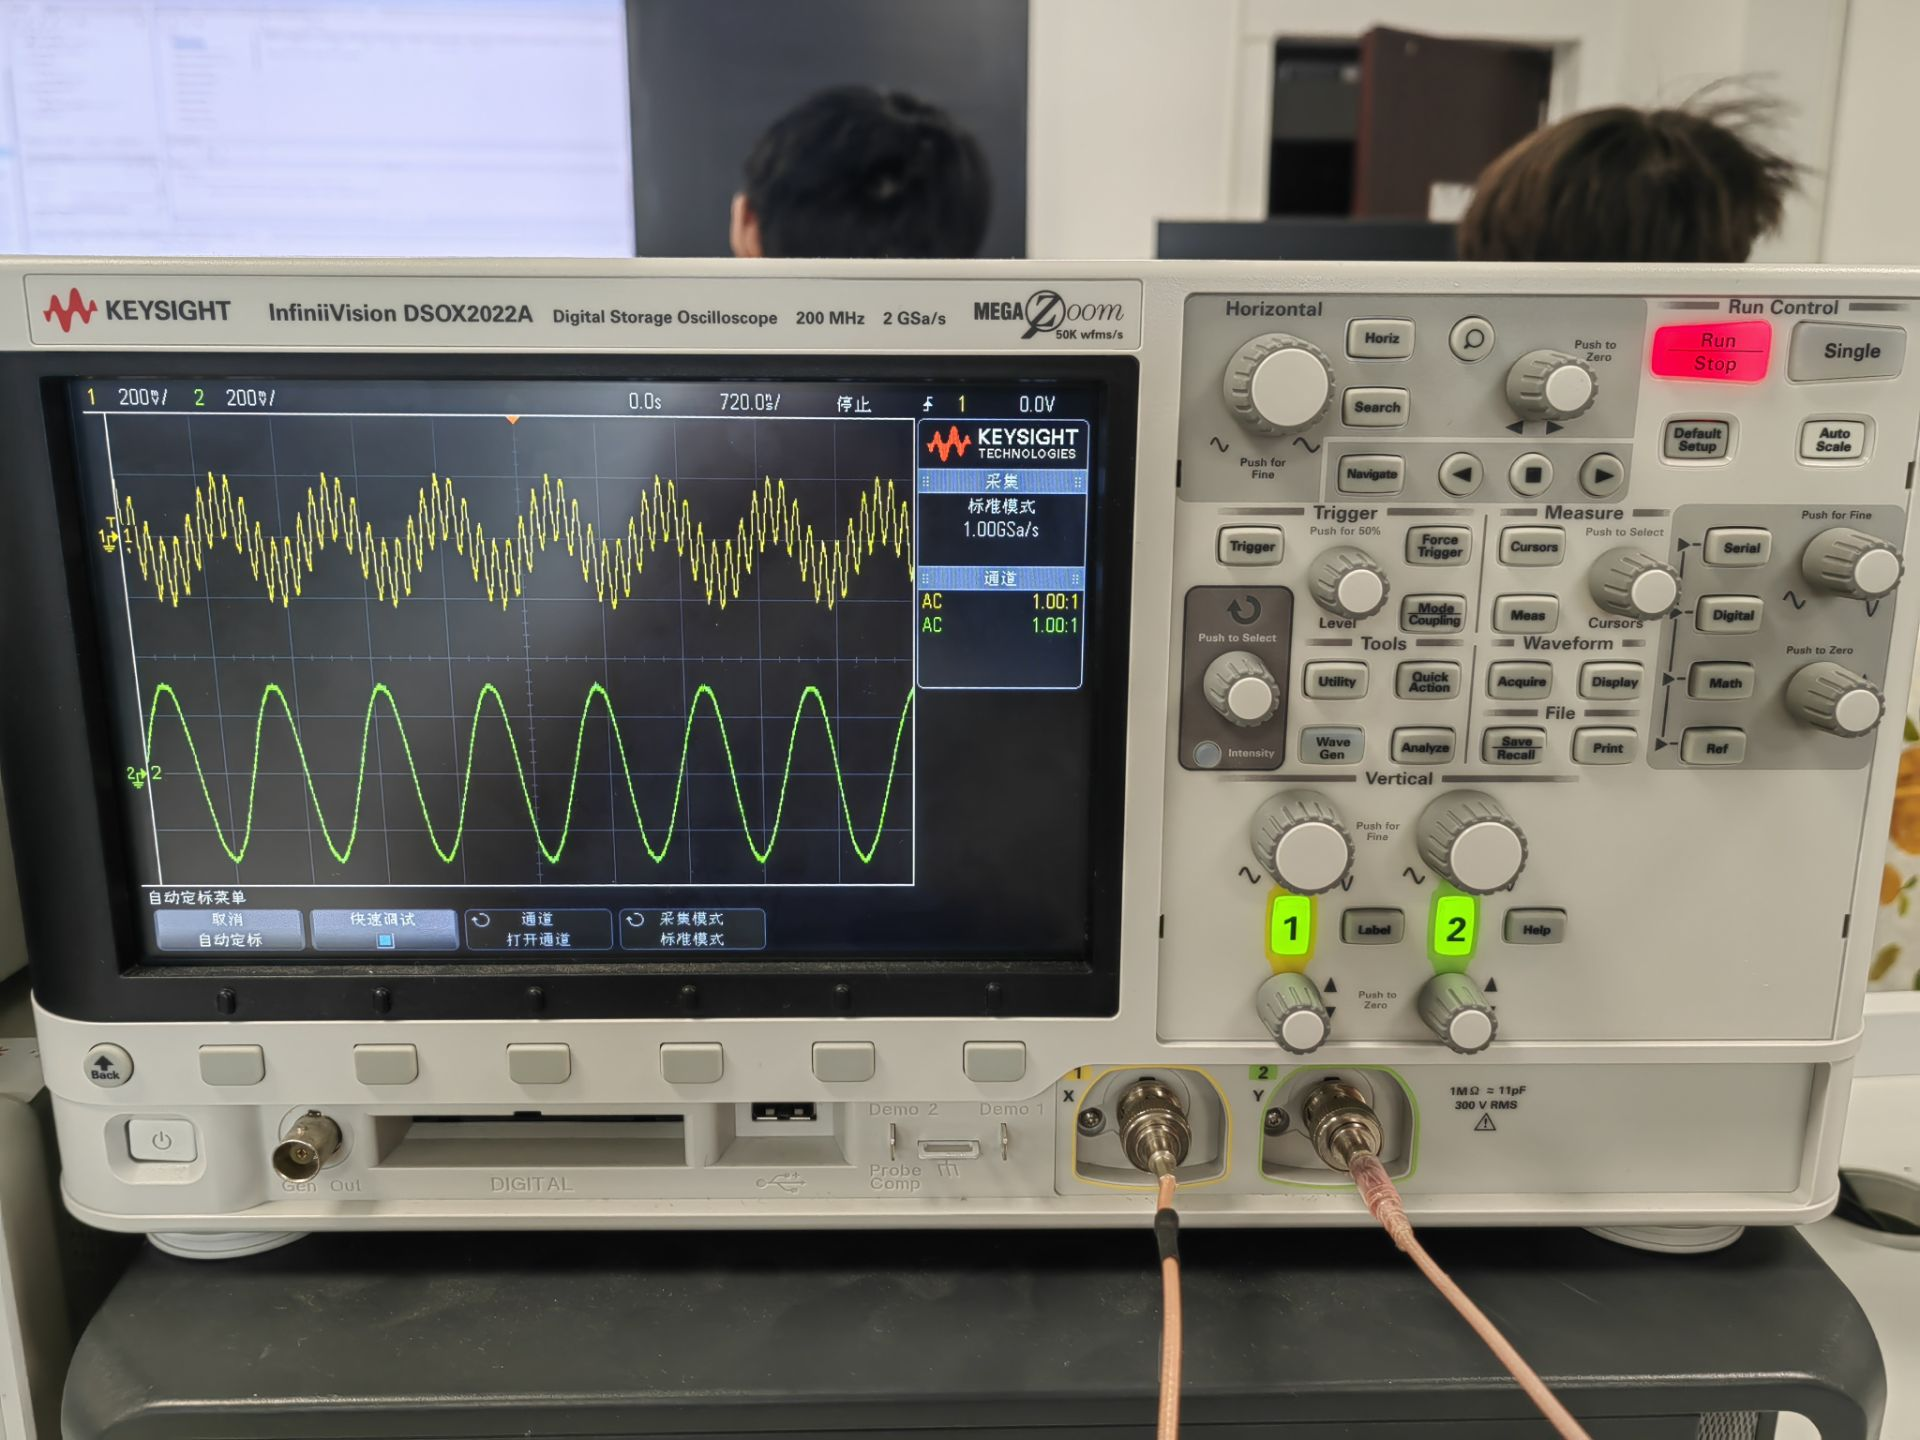
\includegraphics[width = 0.95\textwidth]{figure/exp5/waveform.jpg}
  \caption{滤波前(黄色)与滤波后(绿色)的示波器波形}
  \label{fig:exp5:Implementation}
\end{figure}
\subsection{FPGA资源消耗分析}
首先将该并行滤波器\textbf{设置为顶层模块},并\textbf{禁用}TOP模块。然后通过命令行或\texttt{Add Timing Constraints}绑定时钟管脚\texttt{clk}至50MHz时钟。此时Vivado便可以不通过实际开发板完成资源消耗分析。

完成Implementation后,打开Report Utilization便可看到该模块的资源消耗情况如图~\ref{fig:parrllel:util}。
\begin{figure}[htbp]
  \centering
  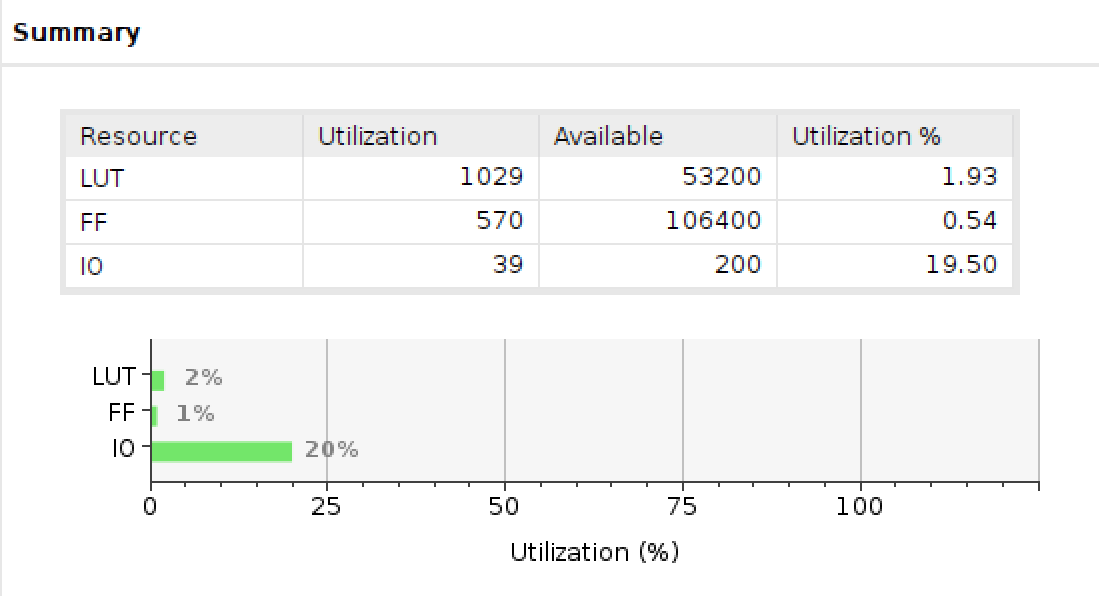
\includegraphics[width=0.55\textwidth]{figure/exp5/util_summary.png}
  \caption{全并行FIR滤波器资源消耗分析}
  \label{fig:parrllel:util}
\end{figure}

该设计的 LUT 和 FF 的资源消耗都很低,但IO资源的消耗较高(19.5\%),这是因为输入输出的位宽较大,属于刚性需求。并且可以看出,在Implementation的过程中,布线器对资源进行了优化。总消耗资源并不等于每个子模块的资源消耗之和。

\subsection{时序检查报告}

图~\ref{fig:exp5:timing}~展示了FPGA设计的时序总结,包括Setup、Hold和Pulse Width三个方面的时序检查结果。

\begin{figure}[htbp]
  \centering
  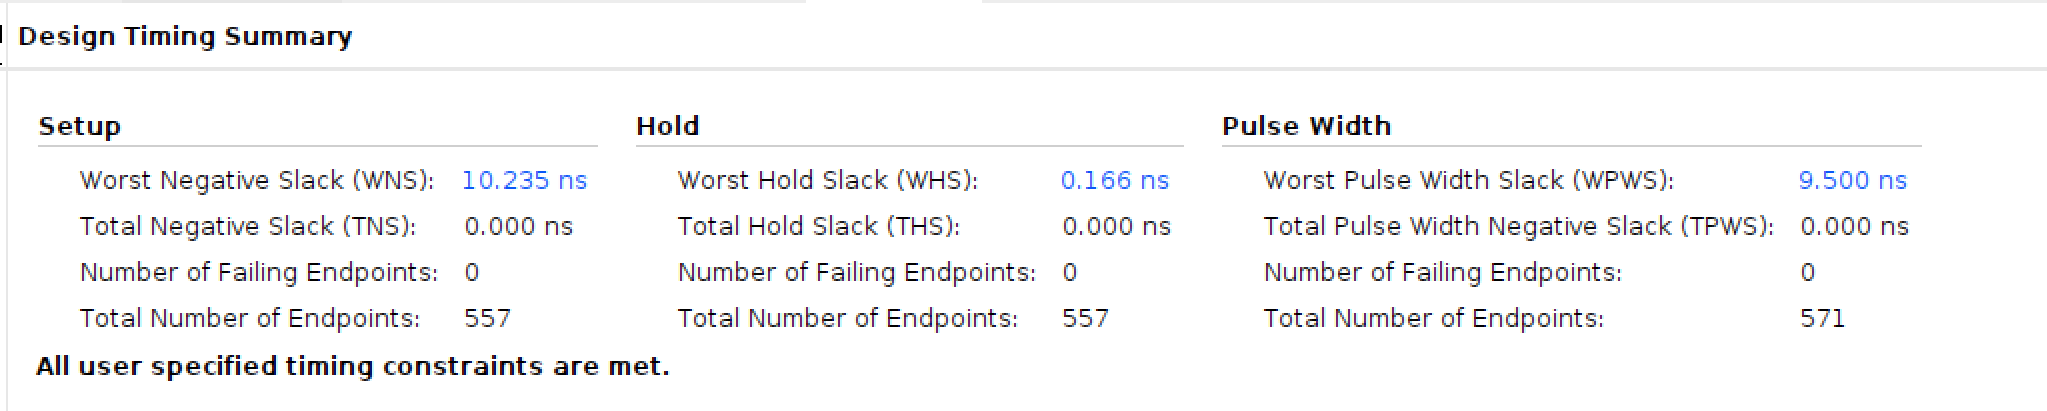
\includegraphics[width=0.75\textwidth]{figure/exp5/timing_summary.png}
  \caption{模块时序检查报告}
  \label{fig:exp5:timing}
\end{figure}


\textbf{Setup:}  
\begin{itemize}
  \item Worst Negative Slack (WNS): 10.235 ns。表示最差的负时序余量,值为10.235纳秒,说明在时序上存在一定的余量,设计没有违反时序约束。  
\item Total Negative Slack (TNS): 0.00 ns。表示总的负时序余量为零,说明所有时序约束都被满足。  
\item Number of Failing Endpoints: 0。表示没有时序失败的端点,所有的时序约束都符合要求。  
\item Total Number of Endpoints: 557。表示在设计中,共有557个时序端点。
\end{itemize}


\textbf{Hold:}  
\begin{itemize}
\item Worst Hold Slack (WHS): 0.166 ns。表示最差的保持时序余量,值为0.166纳秒,表明该设计在保持时序方面没有违反约束。  
\item Total Hold Slack (THS): 0.00 ns。表示总的保持时序余量为零,表明所有保持时序约束都被满足。  
\item Number of Failing Endpoints: 0。表示没有违反保持时序约束的端点。  
\item Total Number of Endpoints: 557。表示共有557个端点。
\end{itemize}

\textbf{Pulse Width:}  
\begin{itemize}
  \item Worst Pulse Width Slack (WPWS): 9.500 ns。表示最差的脉冲宽度时序余量,值为9.500纳秒,说明设计在脉冲宽度方面有足够的时序余量。  
  \item Total Pulse Width Negative Slack (TPWS): 0.00 ns。表示总的脉冲宽度负时序余量为零,表明所有脉冲宽度时序约束都得到满足。  
  \item Number of Failing Endpoints: 0。表示没有违反脉冲宽度时序约束的端点。  
\item Total Number of Endpoints: 571。表示共有571个端点。
\end{itemize}


\textbf{总结:}  
所有用户指定的时序约束都已满足,设计没有违反时序约束,时序余量充足,表明该设计的时序性能良好,符合要求。

\section{思考与讨论}
\subsection{提高该滤波器工作频率的方法}

由于全并行、全展开结构下,大部分逻辑均能在一个时钟周期内完成,因此耗时较久的即为乘法器模块。为了提升乘法器的效率,可以使用以下两种办法:
\begin{enumerate}
  \item 使用DSP资源中的乘法单元代替LUT。
  \item 增加乘法器的并行度。
\end{enumerate}

\chapter{串行结构的FIR滤波器设计}
\begin{introduction}
    \item \textit{通过滤波器设计工具确定滤波器系数;}
    \item \textit{Verilog编写串行结构FIR滤波器;}
    \item \textit{基于串行结构的FIR滤波器FPGA实现。}
\end{introduction}
\section{实验背景与目的}

\section{实验原理}

\section{实验使用软件/平台}
\begin{itemize}
    \item Xilinx Vivado 2024.2;
    \item eNodeX 30B软件无线电创新平台;
    \item 示波器。
    \item MATLAB \& Simulink R2024b;
  \end{itemize}
\section{实验内容}
\subsection{FIR滤波器系数确定}
打开MATLAB的\textcolor{b!50}{Filter Designer},进行如图~\ref{fig:filterdesign}~配置:
\begin{figure}
    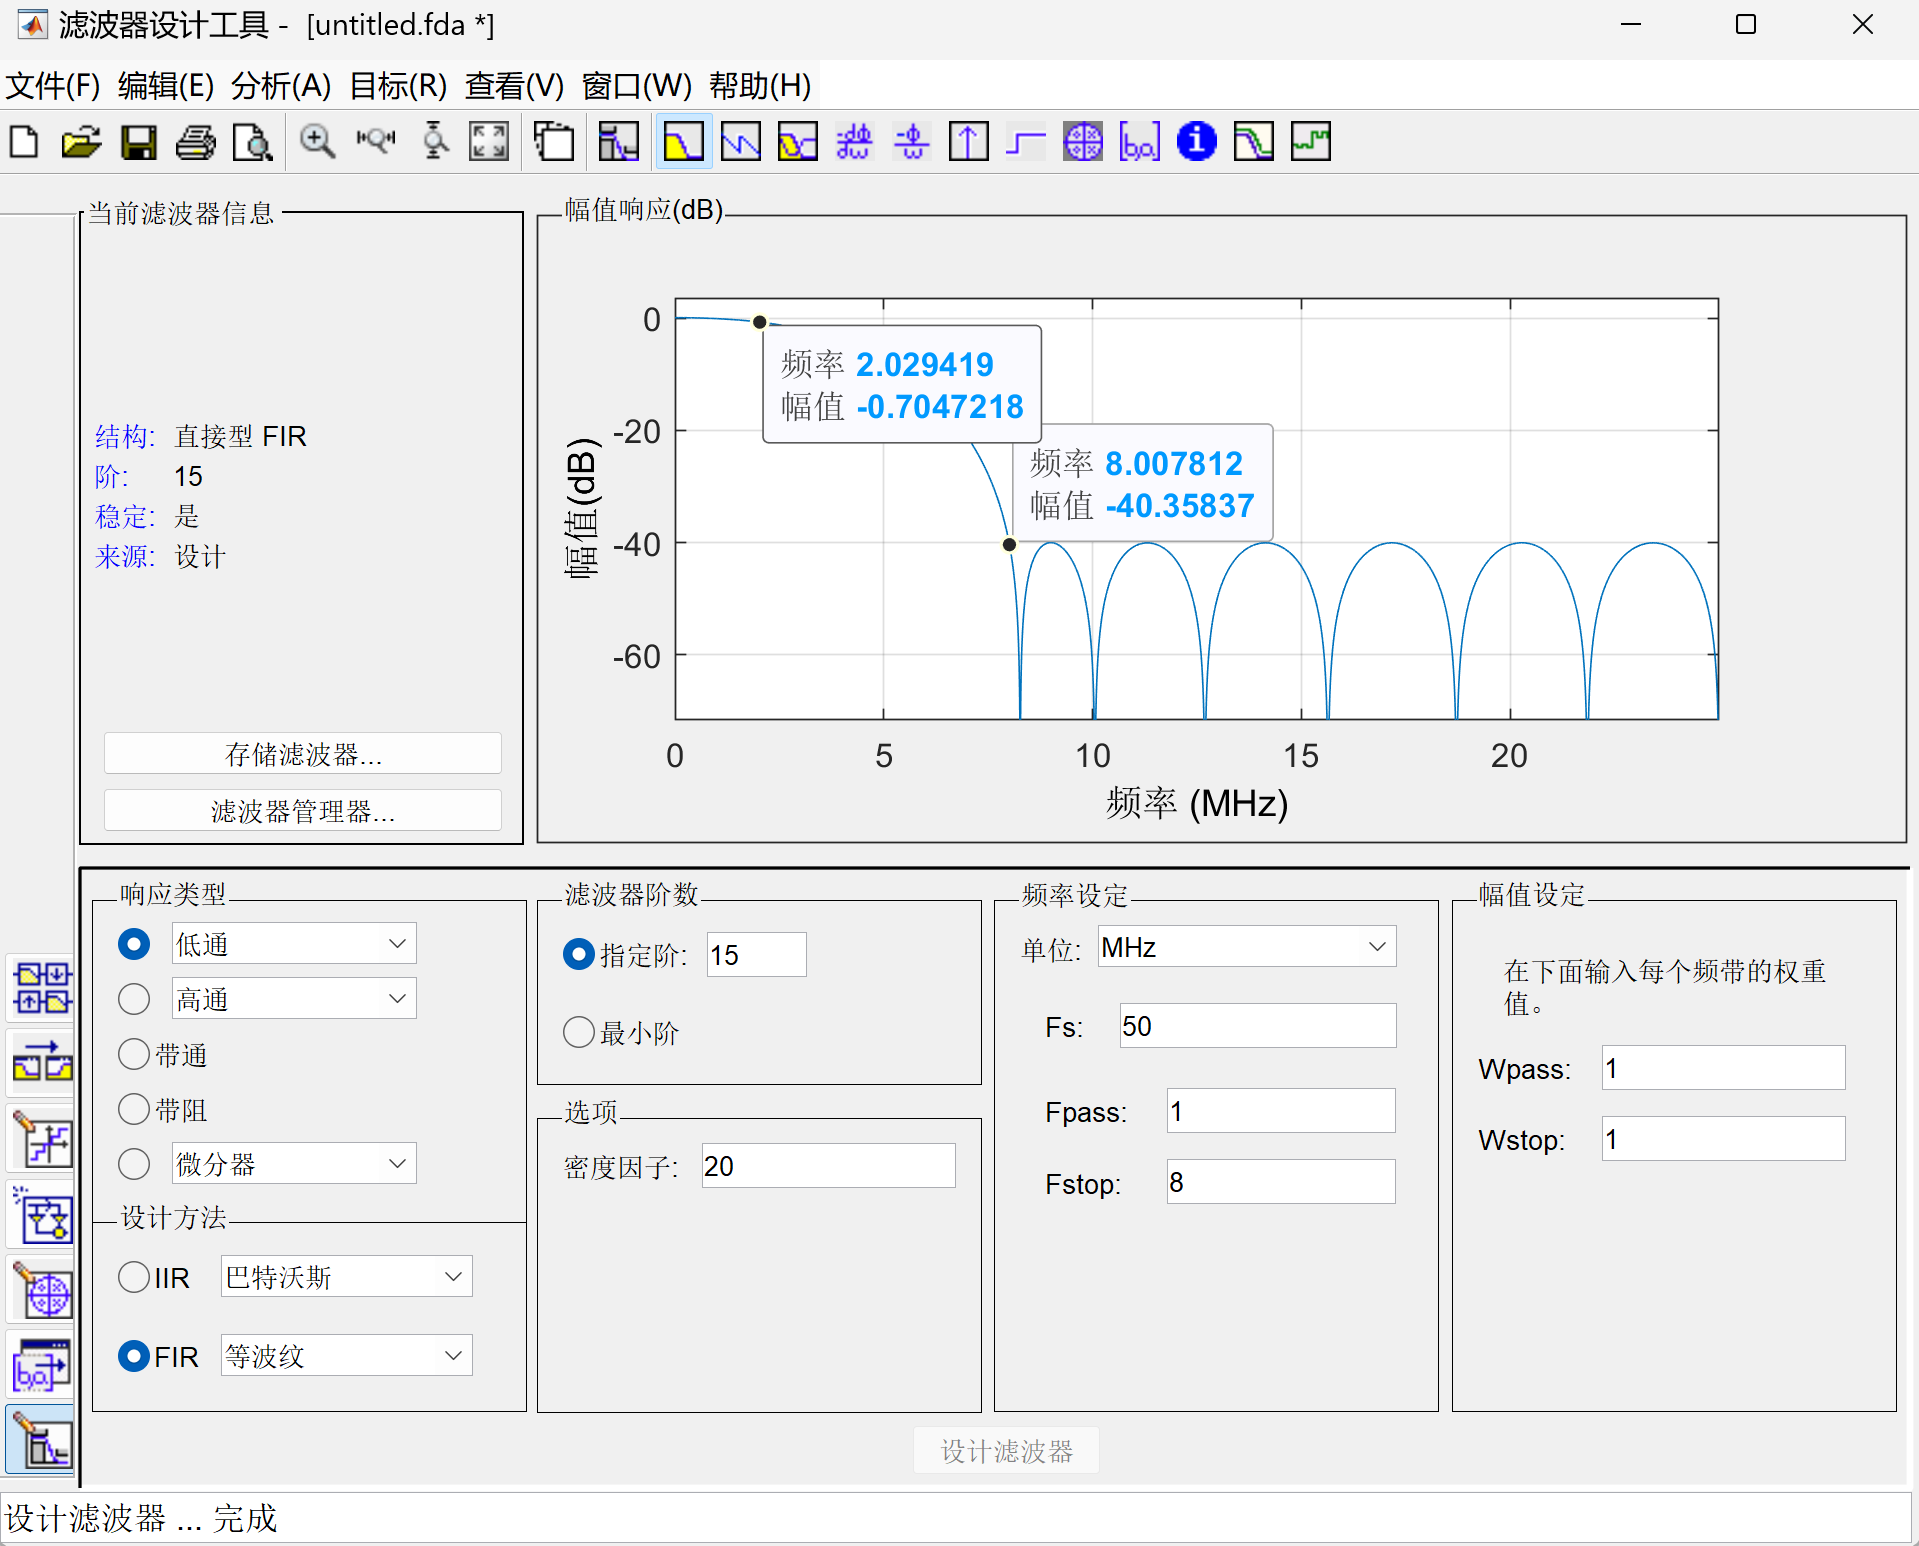
\includegraphics[width=0.45\textwidth]{figure/exp6/filter_designer.png}
    \caption{滤波器系数确定}
    \label{fig:filterdesign}
\end{figure}

在采样频率为50MHz时,该滤波器的通带边界为1MHz,阻带边界为8MHz,可以滤除
\subsection{串行结构FIR滤波器FPGA实现}
滤波器仿真结束后,连接TOP模块进行板级仿真。此次实验中,模拟输入信号由eNodeX ADC模块输入至主模块中,主模块处理好后再进行DAC输出。由于eNode X 仅有2个I/O接口,因此示波器只能显示1路信号。
\begin{lstlisting}[language=verilog,caption={TOP模块}]
`timescale 1ns / 1ps
module TOP (
    // DAC PINS
    output signed [13:0] LS_DAC2_DB,   // DA 数据2
    output               LS_DAC2_CLK,  // DA 时钟2
    output               LS_DAC2_WRT,  // DA 输出写信号,同时钟信号
    output signed [13:0] LS_DAC1_DB,   // DA 数据1
    output               LS_DAC1_CLK,  // DA 时钟1
    output               LS_DAC1_WRT,  // DA 输出写信号,同时钟信号

    output LS_DAC_MODE,

    // ADC PINS
    // input [13:0] LS_ADC2_DB, LS_ADC1_DB,     // AD 采样数据输入,目前是用的12bit ADC
    // input  LS_ADC2_OTR, LS_ADC1_OTR,         // AD 采样溢出指示(最大输入幅??2V??
    // output LS_ADC2_CLK, LS_ADC1_CLK,         // AD 采样时钟
    input [11:0] LS_ADC1_DB,
    output LS_ADC1_CLK,


    // GPIOS Ports
    // output GPIO_TH1, GPIO_TH2, GPIO_TH3, GPIO_TH4, GPIO_TH5,
    // output GPIO_TH6, GPIO_TH7, GPIO_TH8, GPIO_TH9, GPIO_TH10

    input PL_CLK_100MHz
);
  reg signed [11:0] adc1_data;

  // ADC Sampling Frequency is 6.25MHz
  always @(posedge clk_6_25M) begin
    adc1_data <= LS_ADC1_DB;
  end


  wire               clk_50M;
  wire               clk_6_25M;
  wire               clk_locked;
  wire signed [10:0] sin250k;
  wire signed [10:0] sin1M;
  wire signed [11:0] xin;
  wire signed [25:0] yout;

  clk50m inst_clk50m (
      // Clock out ports
      .clk_out_50m(clk_50M),       // output clk_out_50m
      .clk_out_625  (clk_6_25M),     // output clk_6_25M
      // Status and control signals
      .locked     (clk_locked),    // output locked
      // Clock in ports
      .clk_in1    (PL_CLK_100MHz)  // input clk_in1
  );

  ila_0 inst_ila (
      .clk(clk_50M),
      .probe0(adc1_data),
      .probe1(yout[25:12]),
      .probe2(xin)
  );



  fir_serial sim (
      .rst (!clk_locked),
      .clk (clk_50M),
      .Xin (adc1_data),
      .Yout(yout)
  );

  SIN_1M sin_1M (
      .aclk                (clk_50M),  // input wire aclk
      .s_axis_config_tvalid(1'b1),     // input wire s_axis_config_tvalid
      .s_axis_config_tdata (16'H51E),  // input wire [11 : 0] s_axis_config_tdata
      .m_axis_data_tvalid  (),         // output wire m_axis_data_tvalid
      .m_axis_data_tdata   (sin1M)     // output wire [11 : 0] m_axis_data_tdata
  );
  SIN_1M sin_0_25M (
      .aclk                (clk_50M),  // input wire aclk
      .s_axis_config_tvalid(1'b1),     // input wire s_axis_config_tvalid
      .s_axis_config_tdata (16'H147),  // input wire [15 : 0] s_axis_config_tdata
      .m_axis_data_tvalid  (),         // output wire m_axis_data_tvalid
      .m_axis_data_tdata   (sin250k)   // output wire [15 : 0] m_axis_data_tdata
  );

  // 计算输入信号
  assign xin = sin1M + sin250k;
  // DAC OUTPUT
  assign LS_DAC_MODE = 1'b1;
  assign LS_DAC1_DB = {{2{xin[11]}}, xin} + 14'h2000;  // to unsigned
  assign LS_DAC1_CLK = !clk_50M;
  assign LS_DAC1_WRT = LS_DAC1_CLK;
  assign LS_DAC2_DB = yout[25:12] + 14'h2000;  // to unsigned
  assign LS_DAC2_CLK = clk_50M;
  assign LS_DAC2_WRT = LS_DAC2_CLK;

  assign LS_ADC1_CLK = clk_6_25M;
endmodule

\end{lstlisting}
\subsection{FPGA资源消耗分析}
首先将该并行滤波器\textbf{设置为顶层模块},并\textbf{禁用}TOP模块。然后通过命令行或\texttt{Add Timing Constraints}绑定时钟管脚\texttt{clk}至50MHz时钟。此时Vivado便可以不通过实际开发板完成资源消耗分析。

完成Implementation后,打开Report Utilization便可看到该模块的资源消耗情况如图~\ref{fig:exp6:util}。
\begin{figure}[htbp]
  \centering
  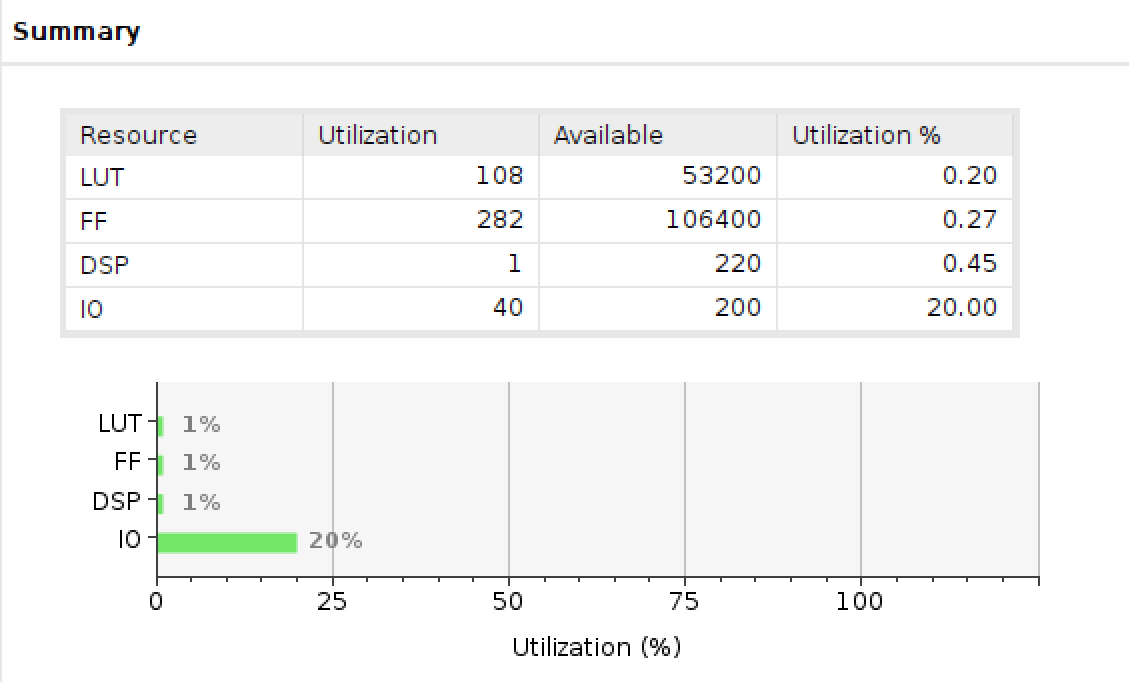
\includegraphics[width=0.55\textwidth]{figure/exp6/util_summary.png}
  \caption{串行结构FIR滤波器资源消耗分析}
  \label{fig:exp6:util}
\end{figure}

该设计的 LUT 和 FF 的资源消耗都很低,但IO资源的消耗较高(20\%),这是因为输入输出的位宽较大,属于刚性需求。并且可以看出,在Implementation的过程中,布线器对资源进行了优化。总消耗资源并不等于每个子模块的资源消耗之和。

\subsection{时序检查报告}

图~\ref{fig:exp6:timing}~展示了FPGA设计的时序总结,包括Setup、Hold和Pulse Width三个方面的时序检查结果。

\begin{figure}[htbp]
  \centering
  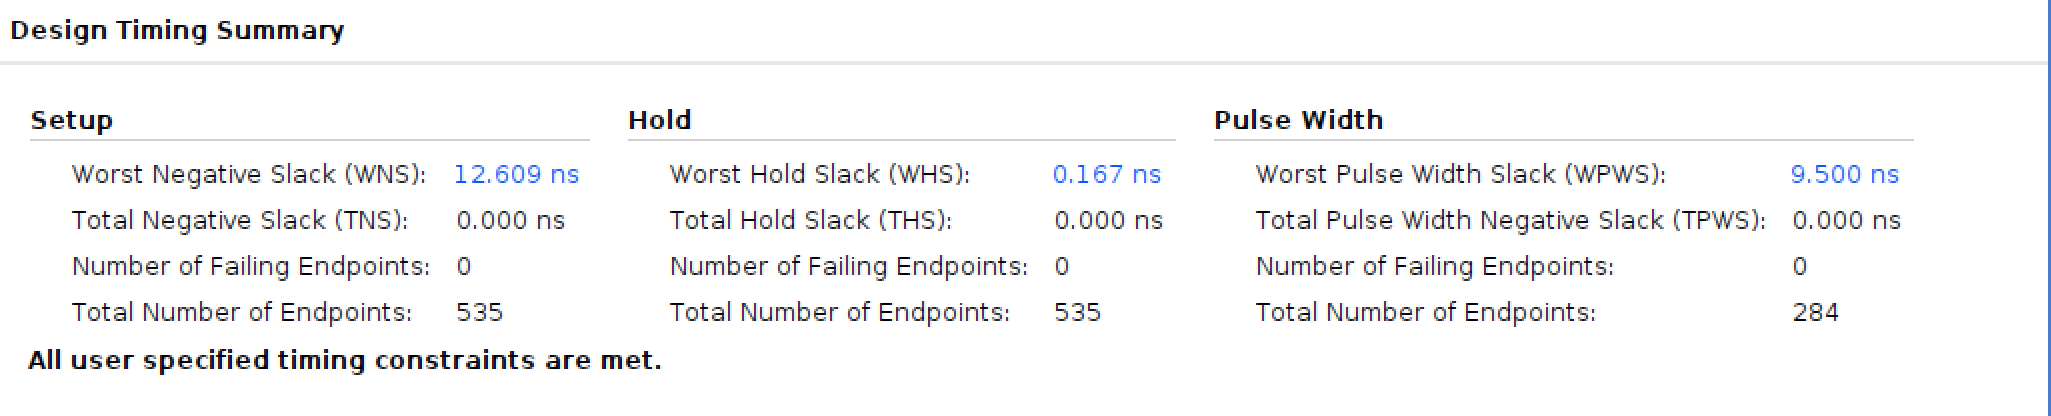
\includegraphics[width=0.75\textwidth]{figure/exp6/timing_summary.png}
  \caption{模块时序检查报告}
  \label{fig:exp6:timing}
\end{figure}


\textbf{Setup:}  
\begin{itemize}
  \item Worst Negative Slack (WNS): 12.635 ns。表示最差的负时序余量,值为12.635纳秒,说明在时序上存在一定的余量,设计没有违反时序约束。  
\item Total Negative Slack (TNS): 0.00 ns。表示总的负时序余量为零,说明所有时序约束都被满足。  
\item Number of Failing Endpoints: 0。表示没有时序失败的端点,所有的时序约束都符合要求。  
\item Total Number of Endpoints: 535。表示在设计中,共有535个时序端点。
\end{itemize}


\textbf{Hold:}  
\begin{itemize}
\item Worst Hold Slack (WHS): 0.167 ns。表示最差的保持时序余量,值为0.167纳秒,表明该设计在保持时序方面没有违反约束。  
\item Total Hold Slack (THS): 0.00 ns。表示总的保持时序余量为零,表明所有保持时序约束都被满足。  
\item Number of Failing Endpoints: 0。表示没有违反保持时序约束的端点。  
\item Total Number of Endpoints: 535。表示共有535个端点。
\end{itemize}

\textbf{Pulse Width:}  
\begin{itemize}
  \item Worst Pulse Width Slack (WPWS): 9.500 ns。表示最差的脉冲宽度时序余量,值为9.500纳秒,说明设计在脉冲宽度方面有足够的时序余量。  
  \item Total Pulse Width Negative Slack (TPWS): 0.00 ns。表示总的脉冲宽度负时序余量为零,表明所有脉冲宽度时序约束都得到满足。  
  \item Number of Failing Endpoints: 0。表示没有违反脉冲宽度时序约束的端点。  
\item Total Number of Endpoints: 284。表示共有284个端点。
\end{itemize}


\textbf{总结:}  
所有用户指定的时序约束都已满足,设计没有违反时序约束,时序余量充足,表明该设计的时序性能良好,符合要求。

\section{思考与讨论}
\subsection{半串行结构FIR滤波器}
为了提高工作频率,采用两个乘法器和两个加法器完成FIR滤波器的设计。此时设计的滤波器代码为:
\begin{lstlisting}[language=verilog]
module FIR_HALF_SERIAL (
    input rst,  // Async reset on posedge            
    input clk,  // system clock                    
    input signed [11:0] Xin,  // 12-bit input
    output reg signed [25:0] Yout  // adder output
);
  reg signed [11:0] coe_a, coe_b;  // coefficients for two separate operations
  wire signed [12:0] add_s1, add_s2;  // intermediate adders' results

  reg [2:0] count = 3'd0;  
  always @(posedge clk or posedge rst) begin
    if (rst) count <= 3'd0;
    else begin
      if (count == 3'd4) begin
        count <= 0;
      end else begin
        count <= count + 1;
      end
    end
  end

  reg [11:0] Xin_Reg[15:0];  // Data shift register
  // reg [3:0] i, j; 

  // Store data into the shift register
  always @(posedge clk or posedge rst) begin
    if (rst) begin
      // Initialize register values to 0
      Xin_Reg[0]  <= 12'd0;
      Xin_Reg[1]  <= 12'd0;
      Xin_Reg[2]  <= 12'd0;
      Xin_Reg[3]  <= 12'd0;
      Xin_Reg[4]  <= 12'd0;
      Xin_Reg[5]  <= 12'd0;
      Xin_Reg[6]  <= 12'd0;
      Xin_Reg[7]  <= 12'd0;
      Xin_Reg[8]  <= 12'd0;
      Xin_Reg[9]  <= 12'd0;
      Xin_Reg[10] <= 12'd0;
      Xin_Reg[11] <= 12'd0;
      Xin_Reg[12] <= 12'd0;
      Xin_Reg[13] <= 12'd0;
      Xin_Reg[14] <= 12'd0;
      Xin_Reg[15] <= 12'd0;
    end else begin
      if (count == 3'd4) begin
        // Shift data in the register every time count == 4
        Xin_Reg[15] <= Xin_Reg[14];
        Xin_Reg[14] <= Xin_Reg[13];
        Xin_Reg[13] <= Xin_Reg[12];
        Xin_Reg[12] <= Xin_Reg[11];
        Xin_Reg[11] <= Xin_Reg[10];
        Xin_Reg[10] <= Xin_Reg[9];
        Xin_Reg[9]  <= Xin_Reg[8];
        Xin_Reg[8]  <= Xin_Reg[7];
        Xin_Reg[7]  <= Xin_Reg[6];
        Xin_Reg[6]  <= Xin_Reg[5];
        Xin_Reg[5]  <= Xin_Reg[4];
        Xin_Reg[4]  <= Xin_Reg[3];
        Xin_Reg[3]  <= Xin_Reg[2];
        Xin_Reg[2]  <= Xin_Reg[1];
        Xin_Reg[1]  <= Xin_Reg[0];
        Xin_Reg[0]  <= Xin;
      end
    end
  end


  reg signed [11:0] add_a1, add_b1, add_a2, add_b2;

  always @(posedge clk or posedge rst) begin
    if (rst) begin
      add_a1 <= 12'd0;
      add_b1 <= 12'd0;
      add_a2 <= 12'd0;
      add_b2 <= 12'd0;
      coe_a  <= 12'd0;
      coe_b  <= 12'd0;
    end else begin
      // Select different coefficients for two separate operations based on the count value
      case (count)
        3'd0: begin
          add_a1 <= Xin_Reg[0];
          add_b1 <= Xin_Reg[15];
          coe_a  <= -12'd116;  // c0
          add_a2 <= Xin_Reg[1];
          add_b2 <= Xin_Reg[14];
          coe_b  <= -12'd111;  // c1
        end
        3'd1: begin
          add_a1 <= Xin_Reg[2];
          add_b1 <= Xin_Reg[13];
          coe_a  <= -12'd22;  // c2
          add_a2 <= Xin_Reg[3];
          add_b2 <= Xin_Reg[12];
          coe_b  <= 12'd243;  // c3
        end
        3'd2: begin
          add_a1 <= Xin_Reg[4];
          add_b1 <= Xin_Reg[11];
          coe_a  <= 12'd692;  // c4
          add_a2 <= Xin_Reg[5];
          add_b2 <= Xin_Reg[10];
          coe_b  <= 12'd1239;  // c5
        end
        3'd3: begin
          add_a1 <= Xin_Reg[6];
          add_b1 <= Xin_Reg[9];
          coe_a  <= 12'd1743;  // c6
          add_a2 <= Xin_Reg[7];
          add_b2 <= Xin_Reg[8];
          coe_b  <= 12'd2047;  // c7
        end
        default: begin
          add_a1 <= 12'd0;
          add_b1 <= 12'd0;
          coe_a  <= 12'd0;
          add_a2 <= 12'd0;
          add_b2 <= 12'd0;
          coe_b  <= 12'd0;
        end
      endcase
    end
  end

  // Add two separate sums
  ADDER u2_1 (
      .A(add_a1),
      .B(add_b1),
      .S(add_s1)
  );

  ADDER u2_2 (
      .A(add_a2),
      .B(add_b2),
      .S(add_s2)
  );

  wire signed [24:0] Mout1, Mout2;  // Output from two multipliers

  // Two separate multipliers, one for each sum
  MULT u1_1 (
      .CLK(clk),
      .A  (add_s1),
      .B  (coe_a),
      .P  (Mout1)
  );

  MULT u1_2 (
      .CLK(clk),
      .A  (add_s2),
      .B  (coe_b),
      .P  (Mout2)
  );

  reg signed [25:0] sum;

  always @(posedge clk or posedge rst) begin
    if (rst) begin
      sum  <= 26'd0;
      Yout <= 26'd0;
    end else begin
      // Accumulate the results from both multipliers
      sum <= sum + Mout1 + Mout2;
      if (count == 3'd2) begin  // Reset accumulator on count == 2
        Yout <= sum;  // Output the filtered result
        sum  <= 26'd0;  // Clear sum
      end
    end
  end

endmodule
\end{lstlisting}

相较原有代码,新的滤波器频率提高了一倍,然而仿真结果(图~\ref{fig:half_serial}~)显示其低通滤波效果很差。这是因为随着滤波器设计(尤其是采样频率)的改变,滤波器系数需要重新设计。滤波器系数的取值详见MATLAB实验部分,此处不再展开。
\begin{figure}[htbp]
    \includegraphics[width=0.95\textwidth]{figure/exp6/waveform_2adders.png}
    \caption{半串行结构的FIR滤波器滤波效果仿真}
    \label{fig:half_serial}
\end{figure}

\appendix
\chapter{版本更新记录}
本章节记录实验报告集的版本更新记录历史。

\datechange{2025/03/02}{创建实验报告模板}
\begin{change}
  \item 基于 ElegantBook 模板创建实验报告模板;
  \item 完成实验报告封面设计;
  \item 完成实验一报告。
\end{change}

\datechange{2025/03/03}{第二章撰写}
\begin{change}
  \item 完成Verilog仿真。
\end{change}

\datechange{2025/03/09}{第二章撰写}
\begin{change}
\item 完成MATLAB仿真;
\item 完成实验报告。
\end{change}

\datechange{2025/03/10}{第三章撰写}
\begin{change}
\item 完成第三章报告。
\end{change}

\datechange{2025/03/17}{第四章撰写}
\begin{change}
\item 完成硬件和软件部分仿真;
\item 配置Vivado环境;
\item 启动报告撰写。
\end{change}

\datechange{2025/03/18}{第四章撰写}
\begin{change}
\item 独立完成设计硬件综合,修改部分课上代码;
\item 报告撰写。
\end{change}

\datechange{2025/03/24}{第四章撰写}
\begin{change}
  \item 完成硬件仿真。
  \item 报告撰写完成。
\end{change}

\datechange{2025/04/07}{第五章撰写}
\begin{change}
  \item 完成硬件综合并测试波形。
  \item 完成报告撰写。
\end{change}
\end{document}
